

\documentclass{llncs}
\pagestyle{plain}

\usepackage{lineno,hyperref}
\modulolinenumbers[5]

%\journal{Theoretical Computer Science}

%\usepackage{amsmath,amsthm,amssymb,amsfonts,thmtools,thm-restate}
\usepackage{amsmath,amssymb,amsfonts,thmtools,thm-restate}
\usepackage[normalem]{ulem}
\usepackage{tikz}
\usepackage[all]{xy}

%%%%%%%%%%%%%%%%%%%%%%%
%% Elsevier bibliography styles
%%%%%%%%%%%%%%%%%%%%%%%
%% To change the style, put a % in front of the second line of the current style and
%% remove the % from the second line of the style you would like to use.
%%%%%%%%%%%%%%%%%%%%%%%

%% Numbered
%\bibliographystyle{model1-num-names}

%% Numbered without titles
%\bibliographystyle{model1a-num-names}

%% Harvard
%\bibliographystyle{model2-names.bst}\biboptions{authoryear}

%% Vancouver numbered
%\usepackage{numcompress}\bibliographystyle{model3-num-names}

%% Vancouver name/year
%\usepackage{numcompress}\bibliographystyle{model4-names}\biboptions{authoryear}

%% APA style
%\bibliographystyle{model5-names}\biboptions{authoryear}

%% AMA style
%\usepackage{numcompress}\bibliographystyle{model6-num-names}

%% `Elsevier LaTeX' style
%\bibliographystyle{elsarticle-num}
%%%%%%%%%%%%%%%%%%%%%%%


%% Authors' packages, macros, environments
%%%%%%%%%%%%%%%%%%%%%%%
% !TEX root = ./main_TCS.tex

%% PACKAGES
%\usepackage[usenames,dvipsnames]{color}
\usepackage[normalem]{ulem}
\usepackage{amsmath}
%\usepackage{amsthm} 
%\usepackage{amsfonts}
\usepackage{amssymb}
\usepackage{stmaryrd}
\usepackage{subcaption}
%\usepackage{graphicx} 
 \usepackage[all]{xy}
\usepackage{bussproofs}
\usepackage{mathtools} 
\usepackage{wasysym}
\usepackage{lscape}
\usepackage{graphicx}
\usepackage{cancel}
\newcommand{\plusarrow}{\xrightarrow{+\Delta V \%}}

\newcommand{\CNA}{\textsf{CNA}}

%% LINK CALCULUS
\newcommand{\link}[2]{\ensuremath{{}^{#1} \backslash_{#2}^{}}}
\newcommand{\chainedlink}[2]{\ensuremath{\backslash_{#1}^{#2}}}
\newcommand{\startchain}[1]{\ensuremath{{}^{#1}_{}}}
\newcommand{\chainend}[1]{\ensuremath{\backslash_{#1}^{}}}
%\newcommand{\midlink}[2]{\ensuremath{{}_{#1} {}^{#2}}}
\newcommand{\midlink}[2]{\ensuremath{{}_{#1}^{#2}}}
\newcommand{\silent}{\tau}
%\newcommand{\noact}{*}
%\newcommand{\noact}{_{\square}}
\newcommand{\noact}{\scriptstyle {\square}}
\newcommand{\noacts}{\scriptstyle \square}
\newcommand{\merges}[2]{\ensuremath{#1 \bullet   #2}}
%\newcommand{\merges}[2]{\ensuremath{#1 \,\wr\, #2}}
\newcommand{\restrict}[1]{\ensuremath{(\nu\, #1)}}
\newcommand{\recproc}[2]{\ensuremath{\mathsf{rec}\ #1.\, #2}}
\newcommand{\nil}{\mathbf{0}}
%\newcommand{\solid}[1]{\ensuremath{\{\, #1\,\}}}
\newcommand{\tuple}[1]{\ensuremath{\langle #1\rangle}}
\newcommand{\variable}[1]{\ensuremath{\underline{#1}}}
%\newcommand{\subst}[2]{#2 \mapsto #1}
\newcommand{\subst}[2]{#1/#2}
\newcommand{\ground}[1]{\ensuremath{\llbracket\, #1 \,\rrbracket}}
\newcommand{\values}[1]{\ensuremath{\mathit{vals}(#1)}}
\newcommand{\variables}[1]{\ensuremath{\mathit{vars}(#1)}}
\newcommand{\extruded}[1]{\ensuremath{\mathit{ex}(#1)}}
\newcommand{\innames}[1]{\ensuremath{\mathit{in}(#1)}}
\newcommand{\outnames}[1]{\ensuremath{\mathit{out}(#1)}}
\newcommand{\names}[1]{\ensuremath{\mathit{names}(#1)}}
\newcommand{\forwarded}[1]{\ensuremath{\llparenthesis #1\rrparenthesis}}
\newcommand{\instanceof}{\preceq}
\newcommand{\elc}{\ensuremath{\epsilon}}
\newcommand{\reduce}[1]{\ensuremath{\mathsf{e}(#1)}}
%\newcommand{\stretcheq}{\ensuremath{\bowtie}}
\newcommand{\stretcheq}{\scriptsize \mathrel \vartriangleright \joinrel \mathrel \vartriangleleft}
%$\mathrel \vartriangleright \joinrel \mathrel \vartriangleleft$
%\newcommand{\blackstretcheq}{\ensuremath{\fbowtie}}
%\newcommand{\llink}{\ensuremath{\mathrel \square \joinrel \mathrel \square}}
\newcommand{\blackstretcheq}{\mathrel{\scriptsize {\mathrel \blacktriangleright \joinrel \mathrel \blacktriangleleft}}}
%$\mathrel \blacktriangleright \joinrel \mathrel \blacktriangleleft$
\newcommand{\simnet}{\ensuremath{\stackrel{\stretcheq}{\sim}}}
\newcommand{\simbnet}{\ensuremath{\stackrel{\blackstretcheq}{\sim}}}

\newcommand{\solid}[1]{{#1}\downarrow}
\newcommand{\notsolid}[1]{{#1}\ndownarrow}

\newcommand{\halfl}[1]{{}^{#1\backslash}}
\newcommand{\halfr}[1]{{}_{\backslash #1}}
\newcommand{\blockchain}[3]{\ensuremath{\left({\big \backslash\!\!\big \backslash}\ {}_{#1}^{\noact}\chainedlink{\noact}{#2}}\right)_{\tiny\begin{array}{l}\\[2pt] \hspace{-42pt}#3\end{array}}\hspace{-0.3cm}}

%% GENERAL
\newcommand{\bn}[1]{\ensuremath{\mathit{bn}(#1)}}
\newcommand{\fn}[1]{\ensuremath{\mathit{fn}(#1)}}
\newcommand{\prodsep}{\;\mid\;}
\newcommand{\defeq}{\triangleq}
\newcommand{\setof}[1]{\{\, #1 \,\}}
\newcommand{\setofmid}[2]{\{\, #1\,\mid\, #2 \,\}}

%% AMBIENT
\newcommand{\nilMA}{\nil}
\newcommand{\incap}[1]{\ensuremath{\mathsf{in}\, #1}}
\newcommand{\outcap}[1]{\ensuremath{\mathsf{out}\, #1}}
\newcommand{\opencap}[1]{\ensuremath{\mathsf{open}\, #1}}
\newcommand{\inprefix}[2]{\ensuremath{\incap{#1}.#2}}
\newcommand{\outprefix}[2]{\ensuremath{\outcap{#1}.#2}}
\newcommand{\openprefix}[2]{\ensuremath{\opencap{#1}.#2}}
\newcommand{\ambient}[2]{\ensuremath{#1 [\, #2\,]}}
\newcommand{\replicated}[1]{\ensuremath{\mathsf{!} #1}}

%% ENCODING
\newcommand{\CNAencode}[2]{\ensuremath{\llbracket\, #1 \,\rrbracket_{#2}}}
\newcommand{\ttop}{{\tt t}}

%% ??
\newcommand{\In}{\, {\cal I}n \, }
\newcommand{\Nin}{\, \not \!\!\!\!{\cal I}n \, }


%%Assertion
\newcommand{\entails}{\models}

% \newtheorem{theorem}{Theorem}
% \newtheorem{lemma}[theorem]{Lemma}
% \newtheorem{proposition}[theorem]{Proposition}
% \newtheorem{corollary}[theorem]{Corollary}
% \newdefinition{definition}[theorem]{Definition}
% \newdefinition{remark}[theorem]{Remark}
% \newdefinition{example}[theorem]{Example}
%\newproof{proof}{Proof}
%%%%%%%%%%%%%%%%%%%%%%%

%%%%% REDUCE VERTICAL SPACING FOR FLOATING FIGURES
\textfloatsep 10pt
\abovecaptionskip 5pt 
\belowcaptionskip\abovecaptionskip

\frenchspacing 
% forza LaTeX ad una spaziatura uniforme, invece di lasciare più spazio
% alla fine dei punti fermi come da convenzione inglese
 
\raggedbottom

\begin{document}

%\begin{frontmatter}

\title{Enhancing reaction systems:\\ a process algebraic approach}
%\title{Embedding Reaction Systems into {\tt link}-calculus}

%% Group authors per affiliation:


% \author[uniss]{Linda Brodo\corref{cor}}
% \ead{brodo@uniss.it}
% 
% \author[unipi]{Roberto Bruni}
% \ead{bruni@di.unipi.it}
% 
% \author[unisi]{Moreno Falaschi}
% \ead{falaschi@unisi.it}
% 
% \address[unipi]{Dipartimento di Informatica, Universit\`{a} di Pisa, Italy}
% \address[uniss]{di Scienze economiche e aziendali,   Universit\`a di Sassari, Italy}
% \address[unisi]{Dipartimento di Ingegneria,   Universit\`a di Siena, Italy}
% 
% \cortext[cor]{Corresponding Author}


\author{ Linda Brodo\inst{1} \and Roberto Bruni\inst{2} \and Moreno 
Falaschi\inst{3}}
\institute{Dipartimento di Scienze economiche e aziendali,
          Universit\`a di Sassari, Italy\\
	   %\email{brodo@uniss.it.} 
	   \and
	   Dipartimento di Informatica,
	   Universit\`{a} di Pisa, Italy\\
	   %\email{bruni@di.unipi.it.} 
	   \and
           Dipartimento di Ingegneria dell'Informazione e Scienze Matematiche\\
           Universit\`a di Siena, Italy
           %\\
           %\email{moreno.falaschi@unisi.it.}
	   }
	   %\date{}
\maketitle


%\end{frontmatter}

\linenumbers

\begin{abstract}
% !TEX root =  main_RS2L_LNCS.tex

In the area of Natural Computing, reaction systems are
a qualitative abstraction inspired by the 
functioning of living cells, suitable to model the main
mechanisms of biochemical reactions.
This model has already been applied
and extended successfully to various areas of research. Reaction 
systems interact with the environment represented by the context, and
pose challenges for further extensions as well as
for the implementation, as it is a new computation model. 
In this paper we consider a variant of the {\tt link}-calculus, which allows to model 
multiparty interaction in concurrent systems, and show that we can
represent reaction systems as processes 
in a modular way, by representing the behaviour of each entity and
preserving faithfully their features. 
We show the correctness and completeness 
of our embedding.
We illustrate our framework by showing the embedding of 
a few examples expressing computer science
and biological applications. 
On top of the LTS semantics for reaction systems provided by our framework, 
we then adapt the classical notion (in concurrency) of bisimulation
to make it more suitable for studying properties of reaction systems.
In particular, we define a new assertion language based on regular expressions, 
which allows to specify the properties of interest, and use it to extend Hennessy-Milner logic
to our framework. Interestingly, the novel notion of bisimilarity and logical equivalence that are defined parametrically on some assertion of interest are proved to coincide, like in the classical case.
Finally, our methodology can contribute to increase the expressiveness
of reaction systems, by exploiting the interaction among 
different reaction systems. 

\end{abstract}

\begin{keywords}
 process algebras, 
 reaction systems,
 multi-party interaction 
\end{keywords}

% !TEX root = ./main_RS2L_LNCS.tex

\section{Introduction}

Natural Computing is an emerging area of research which has two main 
aspects: human designed computing inspired by nature, and computation 
performed in nature. Reaction Systems (RSs)~\cite{BEMR11} are a 
% model of
% formal computation 
rewriting formalism
%model 
inspired by the way biochemical reactions take place in living 
cells.  
This theory has already shown to be relevant in several different 
fields, such as computer science~\cite{MPR15}, 
biology~\cite{ABP14,CMMBM12,Az17,BarbutiGLM16}, 
molecular chemistry~\cite{OY16}.
%,
% and it
%is continuously developing, with a growing number of workshops and
%international meetings. 
Reaction Systems formalise the mechanisms of biochemical systems, 
such as {\em facilitation} and {\em inhibition}. 
As a qualitative approximation of the real biochemical reactions, they
% do not take
%into account the quantity of reagents effectively present. They
consider if a necessary reagent is or not present, and likewise they
consider if an inhibiting molecule is or not present. 
The  possible reactants and inhibitors are called `entities'.
RSs model in a direct way the interaction of a living cell
with the environment (called `context'). However, two RSs are seen
as independent models and do not interact.


%Formally, Reaction Systems are defined as a rewriting formalism.
In this paper, we present an encoding from RSs, 
to the open multiparty process algebra c\CNA,\footnote{After `chained Core Network 
Algebra'.} a variant of the {\tt link}-calculus~\cite{BodeiBB12,BBB17} without name mobility.
This formalism allows several processes to synchronise and 
communicate altogether, at the same time, with a new communicating
mechanism based on links and link chains. 
Our initial motivation for introducing this mechanism was to encode
Mobile Ambients~\cite{CardelliG00}, getting a much stronger operational
correspondence than any available in the literature, such as the one in~\cite{B16}.
 This allowed us to easily encode calculi for biology equipped with membranes, as in~\cite{BodeiBBC14}.
Process calculi have been used successfully to model
biological processes, see~\cite{BBDFH18} for a recent survey.
We illustrate our embedding by means of some simple basic examples,
and then we consider a more complex example, by modeling a RS 
representing a regulatory network for \emph{lac} operon, presented in~\cite{CMMBM12}. We also show that our embedding preserves the main
features of RSs, and prove its correctness and completeness.
Our main contributions are as follows:
\begin{itemize}
\item the behaviour of the context, for each single 
entity,
%\footnote{Entities that belong to the `domain' of a RS.}
can be
specified in a recursive way as an ordinary process;
\item we can express the behaviour of entity mutation,
%change the behaviour of  each single entity $s$  in a
%way that a mutation $s'$ can be expressed; 
in such a way that the mutated entity
$s'$ can  take part to only a subset of rules requiring entity $s$;
\item with a little coding effort, two RSs can
communicate; i.e.  a subset of those entities that the context  can
provide, are then provided by a second RS;
\item as our translation results in  a  c\CNA \ system, from
each state only one transition can be generated, thus the c\CNA \
computation is fully deterministic.
\end{itemize}

The main drawback of our proposal, is that the c\CNA \ translation is
verbose. Nevertheless it is clear that our
translation can be automatised by means of a proper front-end in
an implementation of the {\tt link}-calculus.

As we have remarked, in our translation, Reaction Systems 
get the ability to interact between them in a synchronized manner. 
This interaction is not foreseen in
the basic RS framework, as it can only happen with the context.
By exploiting recursion, the kind of interactions which can be 
defined can be complex and expressive.
Example~\ref{ex:twoRS} and more in general the discussion in 
Section~\ref{sec:discussion} show that 
the interaction between RSs can help to model new scenarios.
\paragraph{Related work}
We are not aware of any inference rules for the RS; it seems not the case
that a deterministic behavior, as the one of the RS, once the initial state is 
fixed, could be defined by inference rules that classically are applied 
to define non-deterministic transition systems.
The reversible computation paradigm for RS extends the RS framework  by
allowing  backward computations as well as forward computations; for this 
goal a set of inference rules for rewriting logic has been 
defined in~\cite{10.1007/978-3-319-73359-3_3}
to exactly keep trace of those elements that  dissolve in the next 
computation step.
 
\paragraph{Structure of the paper.} Section \ref{sec:rs} 
describes RSs and their semantics (interactive processes).
Section \ref{sec:ccna} describes briefly the c\CNA \ process algebra and
its operational semantics.
Section \ref{sec:trans} defines the embedding of RSs in
c\CNA \ processes and shows some simple examples to illustrate 
it.
Section \ref{ex:lactose} shows a more complex example taken from
the literature on RSs and illustrating a \emph{lac} operon.
Section~\ref{sec:discussion} presents some features and 
advantages of our embedding for the compositionality of RSs.
Finally, Section~\ref{sec:conclusion}
discusses future work, and concludes.



% !TEX root = ./main_RS2L_LNCS.tex

\section{Reaction Systems}
\label{sec:rs}

Natural Computing is concerned with human-designed computing inspired by 
nature as well as with computation taking place in nature.
The theory of Reaction Systems~\cite{BEMR11} 
was born in the field of Natural Computing 
to model the behaviour of biochemical reactions taking place in living cells. 
Despite its initial aim, this formalism has shown to be quite useful 
not only for modeling biological phenomena, but also for
the contributions which is giving to computer science~\cite{MPR15}, 
theory of computing, 
mathematics, biology~\cite{ABP14,CMMBM12,Az17,BarbutiGLM16}, 
and molecular chemistry~\cite{OY16}.
%
Here we briefly review the basic notions of RSs, see~\cite{BEMR11} for more details.

The mechanisms that are at the basis of biochemical reactions and thus 
regulate the functioning of a living cell, are 
{\em facilitation} and {\em inhibition}. These mechanisms are 
reflected in the basic definitions of Reaction Systems.

\begin{definition}[Reaction]
A reaction is a triplet $a = (R,I,P)$, where $R, I, P$ are finite,  
non empty sets  and
$R \cap I = \emptyset$. If $S$ is a set such that  $R, I, P \subseteq S$, 
then $a$ is a reaction in $S$.
\end{definition}

The sets $R, I, P$ are also written $R_a, I_a, P_a$ and called the 
\emph{reactant set} of $a$, the  
\emph{inhibitor set} of $a$, and the \emph{product set} of $a$, respectively. 
All reactants are needed for the reaction to take place.
Any inhibitor blocks the reaction if it is present. Products are the outcome of the reaction.
Also,  $R_a \cup I_a$ is the set of the resources of $a$ and $ rac(S)$
denotes the set of all reactions in $S$.
%
Because $R$ and $I$ are non empty, all products are produced from at least one reactant and every reaction can be inhibited in some way. 
Sometimes artificial inhibitors are used that are never produced by any reaction.
For the sake of simplicity, in some examples, we will allow $I$ to be empty.
%Note that since $R_a$ and $I_a$ are both nonempty, we always 
%have $|M_a| \geq 2$.

\begin{definition}[Reaction System]
A Reaction System (RS) is an ordered pair ${\cal A} = (S, A)$ 
such that $S$ is a finite set, and $A \subseteq rac(S)$.
%The set $S$ is called the background (set) of $A$.\\
%The main notion concerning the functioning of a reaction system is defined 
%as follows.
\end{definition}

The set $S$ is called the \emph{background set} of ${\cal A}$, its elements are called \emph{entities},
they represent molecular substances (e.g., atoms, ions, molecules) that may be present
in the states of a biochemical system.
% modeled by $A$. 
The set $A$ is the set of \emph{reactions} of $\mathcal{A}$.
Since $S$ is finite, so is $A$: 
we denote by $|A|$ the number of reactions in $A$.

\begin{definition}[Reaction Result]
Let $W$ be a finite subset of $S$.
\begin{enumerate}
\item Let $a$ be a reaction in $S$. Then $a$ is enabled by $W$, denoted by $\mathit{en}_a(W)$, 
if $R_a \subseteq W$
and $I_a \cap W = \emptyset$. The result of $a$ on $W$, denoted by $\mathit{res}_a(W)$, 
is defined by:
$\mathit{res}_a(W) =P_a$, if $\mathit{en}_a(W)$, and $\mathit{res}_a(W) = \emptyset$ otherwise.
\item Let $A$ be a finite set of reactions. The result of $A$ on $W$, denoted 
by $\mathit{res}_A(W)$,  is defined
by: $\mathit{res}_A(W) = \bigcup_{a \in A} \mathit{res}_a(W)$.
\end{enumerate}
\end{definition}


%\medskip
%\noindent
%{\bf Important Assumptions}\\
The theory of Reaction Systems is based on the following assumptions.
\begin{itemize}
\item {\bf No permanency.} An entity of a set $W$ vanishes unless it is sustained 
by a reaction. This reflects the fact that a living cell would die for lack 
of energy, without chemical reactions.
\item {\bf No counting.} The basic model of RSs is very abstract and 
qualitative, i.e. the quantity of entities that are present 
in a cell is not taken into account. 
%It is just analyzed the behavior of 
%the system based on the reactions that take place.
\item {\bf Threshold nature of resources.} From the 
previous item,
we assume that either an entity is available and there is enough of it 
(i.e. there are no conflicts), or it is not available at all.
\end{itemize}




The dynamic behaviour of a RS is formalized in terms of 
{\em interactive processes}.


\begin{definition}[Interactive Process]
Let ${\cal A} = (S, A)$ be a RS and let $n \geq 0$. 
An $n$-step
\emph{interactive process} in ${\cal A}$ is a pair $\pi = (\gamma, \delta)$ of 
finite sequences s.t.
%
%\begin{center}
$ \gamma=\{C_i\}_{i\in[0,n]}$  and $\delta=\{D_i\}_{i\in[0,n]} $
%$\gamma = C_0, \dots , C_n$ and $\delta = D_0, \dots , D_n$, 
%\end{center}
%\noindent
where 
$ C_{i}, D_{i}  \subseteq S$ for any $i\in[0,n]$, $D_0 = \emptyset$, and 
%$C_0,\dots, C_n, D_0,\dots, D_n  \subseteq S$, $D_0 = \emptyset$, and 
$D_i =  \mathit{res}_{A}(D_{i-1} \cup C_{i-1})$ for any $i \in [1,n]$.
% $i \in \{1,\dots, n\}$.
\end{definition}

Living cells are seen as open systems that continuously react with 
the external environment, in discrete steps. 
The sequence $\gamma$ is the {\em context sequence} of $\pi$ and 
represents the influence of the environment on the Reaction System.
The sequence $\delta$ is
the {\em result sequence} of $\pi$ and it is entirely determined by $\gamma$ and $A$.
%
The sequence $\tau = W_{0}, \ldots, W_{n}$ with $W_{i} = C_{i} \cup D_{i}$, 
for any $i \in [0, n]$
%, and $D_{0} = \emptyset$ 
is called a \emph{state sequence}.
%
Each state $W_{i}$ in a state sequence
is the union of two sets: the context $C_{i}$
at step $i$ and the result $D_i=\mathit{res}_{A}(W_{i-1})$ from the previous step.

%\begin{definition}[State Sequence]
%\label{def:statesequence}
% A {\em state sequence} $\tau$ of an interactive process $\pi$:
%
%\begin{center}
%
%\end{center}
%\end{definition}

%\begin{definition} 
%A process $\pi$, or a state 
%sequence $\tau = W_{0}, \ldots, W_{n}$, is said to be 
%{\em context-independent} when $C_{i} 
%\subseteq D_{i}$, $\forall i \in \{i, \ldots, n \}$.
  %\end{definition}

For technical reasons, we extend the notion of an interactive process to deal with 
infinite sequences.

\begin{definition}[Extended Interactive Process]
Let ${\cal A}=(S,A)$ be a RS, and let $\pi =(\gamma,\delta)$  be an  $n$-step interactive process,
with $ \gamma=\{C_i\}_{i\in[0,n]}$ and  $\delta=\{D_i\}_{i\in[0,n]}$
%, $\delta= D_0, \dots D_n$.
Then, we let $\pi^\infty= (\gamma^\infty,\delta^\infty)$ be the extended interactive process of  $\pi$,
defined as $  \gamma^\infty=\{C_i'\}_{i\in\mathbb{N}}$, $\delta^\infty=\{D_i'\}_{i\in\mathbb{N}}$, where:
$$
C'_j = \left\{
\begin{array}{ll}
C_j & \mbox{if $j\in[0,n]$}\\
\emptyset & \mbox{if $j>n$}
\end{array}
\right.
\qquad
D'_j = \left\{
\begin{array}{ll}
D_0 & \mbox{if $j=0$}\\
\mathit{res}_A(D_{j-1}' \cup C_{j-1}') & \mbox{if ($j\geq 1$)}
\end{array}
\right.
$$
% $C_j' = C_j$ for $j\in[0,n]$ and $C_j' =\emptyset$ for $j>n$,   $D_0' = D_0$ and  $D_j' = \mathit{res}_A(D_{j-1}' \cup C_{j-1}')$ for $j\geq 1$.
\end{definition}

Given an extended interactive process $\pi =(\gamma,\delta)$, we denote by $\pi^k$ the shift of $\pi$ starting at the $k$-th state sequence; formally we let $\pi^k=(\gamma^k,\delta^k)$ with
$\gamma^k=\{C_i'\}_{i\in\mathbb{N}}$, $\delta^k=\{D_i'\}_{i\in\mathbb{N}}$ with 
  $C_0'=C_k \cup D_k$, $D'_0 = \emptyset$, and   $C_i'=C_{i+k}$, $D_i'= D_{i+k}$ for any $i\geq 1$.






%% !TEX root = ./main_RS2L_LNCS.tex


\section{Background on the CNA}



\section{The Core Network Algebra}
\label{sec:network}

In this section we recall the theory of links and link chains to present the syntax and operational semantics of \CNA.
%In this section we just focus on the basic ideas of link interaction, while we shall enhance the model with name mobility in the next section.


\subsection{Syntax}

\begin{definition}
The \CNA\ processes are generated by the following grammar:
\[
\begin{array}{rcl}
P,Q & ::= &
\nil \prodsep
%X \prodsep
\ell. P  \prodsep
P+Q \prodsep
P|Q \prodsep
\restrict{a} P \prodsep
P[\phi] \prodsep
A
\end{array}
\]
\noindent
where $\ell$ is a solid link (i.e.\  $\ell = \link{\alpha}{\beta}$ with $\alpha,\beta\neq \ \noacts$),
$\phi$ is a channel renaming function,
and $A$ is a process identifier for which we assume a definition $A \defeq P$ is available in a given set $\Delta$ of (possibly recursive) process definitions.
\end{definition}

As usual, we write $\tilde{a}$ for tuples of channels and we allow parametric process definitions of the form $A(\tilde{a}) \defeq P$,
where $\tilde{a}$ is the set of free channels of $P$.
For brevity, in the examples, we sometimes write $A \defeq P$ leaving implicit that the free channles of $P$ are the parameters of $A$.
%that
%stand for the set of definitions $\{ A(\tilde{a}) \defeq P[\tilde{a} \slash \tilde{x}]  \;\mid\; \tilde{a}\; \text{ is a tuple of channels} \}$,
%where $\tilde{x}$ is the set of free channels of $P$.

%\begin{remark}
%The extension in which generic link chains are allowed as action prefixes instead of solid links is discussed in Section~\ref{subsec:altdef}.
%\end{remark}

It is evident that processes are built over a CCS-like syntax,
%\footnote{For brevity, we omit the CCS-like renaming operator $P[\Phi]$ because it will be later subsumed by the syntax in Section~\ref{sec:names}).}
with inactive process $\nil$, action prefix $\ell.P$, choice $P+Q$, parallel $P|Q$, restriction $\restrict{a} P$, renaming $P[\phi]$ and constant definition
 $A$, but where the underlying synchronisation algebra~\cite{DBLP:journals/tcs/Winskel84} is based on link chains.
This is made evident by the operational semantics that we present next.

As usual, $\restrict{a}P$ binds the occurrences of $a$ in $P$, the sets of free and of bound names of a process $P$ are defined in the obvious way and 
processes are taken up to alpha-conversion of bound names.
We shall sometimes omit trailing $\nil$, e.g.~by writing $\link{a}{b}$ instead of $\link{a}{b}.\nil$.


\begin{example}
\CNA\ provides us with a natural way to rephrase the communication primitives of usual process calculi, such as CCS and CSP~\cite{Hoare85}, in terms of links.
\begin{itemize}
\item
Intuitively, the output action $\overline{a}$ (resp. the input action $a$) of CCS can be seen as the link $\link{\silent}{a}$
(resp. $\link{a}{\silent}$) and the solid link chain $\startchain{\silent}\chainedlink{a}{a}\chainend{\silent}$  as a dyadic communication, analogous to the silent action $\tau$ of CCS.
% between an output on $a$ (the link $\link{\silent}{a}$) and an input on $a$ (the link $\link{a}{\silent}$).
\item
The action $a$ of CSP can be seen as the link $\link{a}{a}$ and the solid link chain $\startchain{a}\chainedlink{a}{a}\chainedlink{a}{a}\chainend{a}$ as a CSP-like communication among three peers over $a$.
\end{itemize}
\end{example}



%In particular, to implement I/O communication, each link in the whole chain simply carries the same list or tuple of arguments, 
%but with different (send/receive) capabilities. 
%In this way, we keep apart the interaction mechanism from the name-passing one that eventually fit together in synchronisations.
%We have just borrowed from $\pi$-calculus
%the name handling machinery
%(and liberated it from dyadic interaction legacy), still having input, output and extrusion mechanisms.

%In the tuple $t =\tuple{\vec{w}}$, names can be used either as values or as variables. They are distinguished because variables are underlined.
%During communication, variables are instantiated by values, while
%values are used for matching arguments, as in \cite{BodeiBDG10}.
%\begin{example}\label{ex-tuple}
%Consider e.g., the tuples in the two ``complementary'' prefixes $\link{\tau}{a}\tuple{id,n,\variable{x}}.P$ and $\link{a}{\tau}\tuple{id,\variable{y},m}.Q$: the two links can be merged, the first parameters of the tuples must match exactly,
%$n$ is assigned to $y$, while $m$ is assigned to $x$, where
%$\variable{x}$ is an input for $P$, $\variable{y}$ is an input for $Q$, and $id$ is a name known by both processes.
%\end{example}
%This mechanism allows, e.g., a form of multi-way communication, where all peers involved in the chain link can express arguments to be matched and provide actual arguments to replace the formal ones. 

%
%For a tuple $t$, we let $\values{t}$ and $\variables{t}$ denote the set of values and the set of variables of $t$, respectively. 
%We say that a tuple $t$ is \emph{ground} if $\variables{t} = \emptyset$.

%We assume action names are admissible values, i.e.~ as in $\pi$-calculus we have the possibility to communicate (names of) means of communication.
%Similarly to $\restrict{a}$, the prefix $\ell t.P$ binds the occurrences of the variables $\variables{t}$ in $P$ (and the notions of free names $\fn{P}$, bound names $\bn{P}$ and alpha-conversion are updated accordingly).
%In the following, given two set of names $S$ and $T$, we write $S \# T$ as a shorthand for $S\cap T = \emptyset$.

%
%As usual, $\restrict{a}P$ binds the occurrences of $a$ in $P$, the sets of free names and of bound names of a process $P$ are defined in the obvious way and denoted, respectively, by $\fn{P}$ and $\bn{P}$, processes are taken up to alpha-conversion of bound names, and we shall often omit trailing $\nil$, e.g. by writing $\link{a}{b}$ instead of $\link{a}{b}.\nil$ 



% The only original operator is $\solid{P}$ that filters out incomplete communications
% (i.e.~it allows $P$ to evolve only via solid link chains). 

\subsection{Operational Semantics}

The idea is that communication can be routed across several processes by combining the links they make available to form a link chain. Since the length of the link chain is not fixed {\em a priori}, an open multi-party synchronisation is realised.

% We take as observations only link chains whose extremities are silent,
% i.e.~ are in the form $\tau$, because they have not to be composed further. 

%For compositionality reasons, we allow observations to contain
%virtual links $\link{\noact}{\noact}$, to be provided by the context. 

\begin{figure}[t]
\begin{center} 
\begin{prooftree} 
\AxiomC{$s \blackstretcheq \ell $} %\mbox{($\ell$ {\em only} solid link in $s$)}
\RightLabel{\scriptsize(\textit{Act})}
\UnaryInfC{$\ell.P \xrightarrow{v} P$} 
\DisplayProof
\
\AxiomC{$P \xrightarrow{s} P'$} 
\RightLabel{\scriptsize(\textit{Lsum})}
\UnaryInfC{$P+Q \xrightarrow{v} P'$} 
\DisplayProof
\
\AxiomC{$P \xrightarrow{s} P'$} 
\RightLabel{\scriptsize(\textit{Res})}
\UnaryInfC{$\restrict{a}P \xrightarrow{\restrict{a}s} \restrict{a}P'$} 
%\DisplayProof
%\,
%\AxiomC{$Q \xrightarrow{s} Q'$} 
%\RightLabel{\scriptsize(Rsum)}
%\UnaryInfC{$P+Q \xrightarrow{s} Q'$} 
\end{prooftree} 
\end{center}

\begin{center} 
\begin{prooftree} 
\AxiomC{$P \xrightarrow{s} P'$} 
\RightLabel{\scriptsize(\textit{Ren})}
\UnaryInfC{$P[\phi] \xrightarrow{s[\phi]} P'[\phi]$} 
\DisplayProof
\
\AxiomC{$P \xrightarrow{s} P'$} 
\RightLabel{\scriptsize(\textit{Lpar})}
\UnaryInfC{$P|Q \xrightarrow{s} P'|Q$} 
\DisplayProof
\ 
%\AxiomC{$Q \xrightarrow{s} Q'$} 
%\RightLabel{\scriptsize(Rpar)}
%\UnaryInfC{$P|Q \xrightarrow{s} P|Q'$} 
%\end{prooftree} 
%\end{center}
%\begin{center} 
%\begin{prooftree} 
\AxiomC{$P \xrightarrow{s} P'$} 
\AxiomC{$Q \xrightarrow{s'} Q'$} 
\RightLabel{\scriptsize(\textit{Com})}
\BinaryInfC{$P|Q \xrightarrow{\merges{s}{s'}} P'|Q'$} 
\DisplayProof
\end{center}
\begin{center}
%\AxiomC{$P[\subst{\recproc{X}{P}}{X}] \xrightarrow{s} P'$} 
%\RightLabel{\scriptsize(Rec)}
%\UnaryInfC{$\recproc{X}{P} \xrightarrow{s} P'$} 
\AxiomC{$P \xrightarrow{s} P'$}
 \AxiomC{$(A \defeq P)\in\Delta$}
\RightLabel{\scriptsize(\textit{Ide})}
\BinaryInfC{$A \xrightarrow{s} P'$} 
\end{prooftree} 
\end{center}
\caption{SOS semantics of the \CNA\  (rules (\textit{Rsum}) and (\textit{Rpar}) are omitted).}
\label{fig:cnasos}
\end{figure}

The operational semantics is defined in terms of a Labelled Transition System, in which states are \CNA\ processes, labels are link chains, and transitions are generated by the SOS rules in Figure~\ref{fig:cnasos}. 
% 
%%The standard rules \textit{(Rsum)} and \textit{(Rpar)}, symmetric of \textit{(Lsum)} and \textit{(Lpar)} are omitted for brevity.
Notice that the rules are very similar to the ones of CCS, 
apart from the labels that record the link chains involved in the transitions:
moving from dyadic to \emph{linked} interaction does not introduce any complexity burden from the formal point of view.

We comment in details the rules (\textit{Act}), (\textit{Res}), and (\textit{Com}). 
In rules (\textit{Res}) and (\textit{Com}) we leave implicit the side conditions $\restrict{a}s \neq \bot$ and $\merges{s}{s'} \neq \bot$, respectively (they can be easily recovered by noting that otherwise the label of the transition in the conclusion would be undefined).

The rule (\textit{Act}) states that $\ell.P \xrightarrow{s} P$ for any link chain $s$, whose unique solid link is $\ell$,  i.e.\  any $s$ such that $s \blackstretcheq \ell$
(we recall that $s \blackstretcheq \ell$ if $s$ and $\ell$  differ only for the presence of virtual links).
Intuitively, $\ell.P$ can take part in any interaction, in any (admissible) position.
To join in a communication, $\ell.P$ should exhibit the capability to enlarge its link $\ell$ to a link chain $s \blackstretcheq \ell$, whose length is the same as the length of the chains offered by all the other participants, so to proceed with the merge operation. Following the early style, the suitable length is 
%guessed
inferred at the time of deducing the input transition.
Note that, by definition of link chain, if one site of $\ell$ is $\silent$, then $\ell$ can only appear at one of the extremes of $s$.

The rule (\textit{Res}) can serve different aims: 
(i) \emph{floating}, if $a$ does not occur in $s$, then $\restrict{a}s = s$ and  $\restrict{a}P \xrightarrow{s} \restrict{a}P'$;
(ii) \emph{hiding}, if $a$ is matched in $s$ ( i.e.\  $a$ appears as sites already matched by adjacent links), then all occurrences of $a$ in $s$ are transformed to $\silent$ in $\restrict{a}s$;
(iii) \emph{blocking}, if $a$ is pending in $s$ ( i.e.\  there are some
unmatched occurrences of $a$ in $s$), then $\restrict{a}s = \bot$ and the rule cannot be applied.

In the (\textit{Com}) rule the link chains recorded on both the premises' transitions are merged in the conclusion's transition.
This is possible only if $s$ and $s'$ are to some extent ``complementary''.
Contrary to CCS, the rule (\textit{Com}) can appear several times in the proof tree of a transition, because $\merges{s}{s'}$ can still contain virtual links (if $s$ and $s'$ had a virtual link in the same position) and can possibly be merged with other link chains.
However, when $\merges{s}{s'}$ is solid, no further synchronisation is possible (by Lemma~\ref{lemma:solid} (ii)).

%
%A \xrightarrow{a} B. 
%
%
\begin{example}
Let
% $R = \solid{P}$, 
$P = \link{\silent}{a}.P_{1}\ |\ \restrict{b} Q$ and $Q = \link{b}{\silent}.P_{2}\ |\ \link{a}{b}.\nil$, for some processes $P_1$ and $P_2$.
The process $\link{\silent}{a}.P_{1}$ can perform an output on $a$, the process $ \link{b}{\silent}.P_{2}$ can perform an input from $b$; the process $\link{a}{b}$ provides a one-shot link forwarder from $a$ to $b$. 
Their links match along the sequence and a three-party interaction can take place.
Together, these processes can indeed synchronise by agreeing to form the solid link chain
${\startchain{\silent}\chainedlink{a}{a}\chainedlink{\silent}{\silent}\chainend{\silent}}$ of length three, as follows.\footnote{Note that $b$ is restricted and therefore the matched communication on $b$ is replaced by $\tau$ in the observed chain.}


{\small
\begin{center} 
\begin{prooftree} 
\AxiomC{} 
\RightLabel{\scriptsize(\textit{Act})}
\UnaryInfC{$\link{\silent}{a}.P_{1} \xrightarrow{\startchain{\silent}\chainedlink{a}{\noact}\chainedlink{\noact}{\noact}\chainend{\noact}} P_{1}$} 
%
\! \!\!\! \!\!
%\begin{prooftree} 
      \AxiomC{} 
      \RightLabel{\scriptsize(\textit{Act})}
      \UnaryInfC{$\link{b}{\silent}.P_{2} \xrightarrow{\startchain{\noact}\chainedlink{\noact}{\noact}\chainedlink{\noact}{b}\chainend{\silent}} P_{2}$} 
      %
      \AxiomC{} 
      \RightLabel{\scriptsize(\textit{Act})}
      \UnaryInfC{$\link{a}{b}.\nil \xrightarrow{\startchain{\noact}\chainedlink{\noact}{a}\chainedlink{b}{\noact}\chainend{\noact}} \nil$} 
   \RightLabel{\scriptsize(\textit{Com})}
\BinaryInfC{$Q \xrightarrow{\startchain{\noact}\chainedlink{\noact}{a}\chainedlink{b}{b}\chainend{\silent}} P_{2}|\nil$} 
%\end{prooftree} 
%
%\AxiomC{$Q \xrightarrow{\startchain{\noact}\chainedlink{\noact}{a}\chainedlink{b}{b}\chainend{\silent}} P_{2}|\nil$} 
   \RightLabel{\scriptsize(\textit{Res})}
   \UnaryInfC{$\restrict{b}Q \xrightarrow{\startchain{\noact}\chainedlink{\noact}{a}\chainedlink{\silent}{\silent}\chainend{\silent}} \restrict{b} (P_{2}|\nil)$} 
\RightLabel{\scriptsize(\textit{Com})}
\BinaryInfC{$P \xrightarrow{\startchain{\silent}\chainedlink{a}{a}\chainedlink{\silent}{\silent}\chainend{\silent}} P_{1}|\restrict{b} (P_{2}|\nil)$} 
\end{prooftree} 
\end{center}
}

%where
%%
%{\scriptsize
%\begin{center} 
%\begin{prooftree} 
%      \AxiomC{} 
%      \RightLabel{\scriptsize(Act)}
%      \UnaryInfC{$\link{b}{\silent}.P_{2} \xrightarrow{\startchain{\noact}\chainedlink{\noact}{\noact}\chainedlink{\noact}{b}\chainend{\silent}} P_{2}$} 
%      %
%      \AxiomC{} 
%      \RightLabel{\scriptsize(Act)}
%      \UnaryInfC{$\link{a}{b}.\nil \xrightarrow{\startchain{\noact}\chainedlink{\noact}{a}\chainedlink{b}{\noact}\chainend{\noact}} \nil$} 
%   \RightLabel{\scriptsize(Com)}
%\BinaryInfC{$Q \xrightarrow{\startchain{\noact}\chainedlink{\noact}{a}\chainedlink{b}{b}\chainend{\silent}} P_{2}|\nil$} 
%\end{prooftree} 
%\end{center}
%}

%\noindent
%and the suitable chain length, $3$, is inferred and agreed on by all participants.
\end{example}

The following lemma, whose proof goes by rule induction, shows that labels behave like an accordion.
Concretely, any label $s$ in a transition is replaceable with any other chain having a different number of virtual links $\link{\noact}{\noact}$ added to $s$ according to the axioms of $\blackstretcheq$. 
% It is also replaceable with any composition where each $\link{\noact}{\noact}$ inside $s$ is replaced by one or more $\link{\noact}{\noact}$.
The result builds on the previous technical Lemmata~\ref{lem:mergestretch} and~\ref{lemma:res}.
This fact will be later exploited in Section~\ref{abs-sem}, where the abstract semantics is given.



\begin{lemma}[Accordion Lemma]\label{lem:stretchlts}
If $P\xrightarrow{s} P'$ and $s \blackstretcheq s'$,
then $P\xrightarrow{s'} P'$.
\end{lemma}




%\item[(i)]
%If $P\xrightarrow{s} P'$ and $s\link{\noact}{\noact}$ (respectively $\link{\noact}{\noact}s$) is valid,
%then $P\xrightarrow{s\link{\noact}{\noact}} P'$  (respectively $P\xrightarrow{\link{\noact}{\noact}s} P'$).
%\\
%Vice versa, if $P\xrightarrow{s'} P'$ and $s'=s\link{\noact}{\noact}$ or $s'=\link{\noact}{\noact}s$, 
%then $P\xrightarrow{s} P'$.
%
%\item[(ii)]
%If $P\xrightarrow{s_{1}\link{\noact}{\noact}s_{2}} P'$  
%then $P\xrightarrow{s_{1}\startchain{\noact}\chainedlink{\noact}{\noact}\chainend{\noact}s_{2}} P'$.
%\\
%Vice versa, if $P\xrightarrow{s_{1}\startchain{\noact}\chainedlink{\noact}{\noact}\chainend{\noact}s_{2}} P'$ 
%then $P\xrightarrow{s_{1}\link{\noact}{\noact}s_{2}} P'$.
%
%\item[(iii)]
%If $P\xrightarrow{s_{1}\startchain{\alpha}\chainedlink{a}{a}\chainend{\beta}s_{2}} P'$ 
%then $P\xrightarrow{s_{1}\startchain{\alpha}\chainedlink{a}{\noact}\chainedlink{\noact}{a}\chainend{\beta}s_{2}} P'$.
%\\
%Vice versa, if $P\xrightarrow{s_{1}\startchain{\alpha}\chainedlink{a}{\noact}\chainedlink{\noact}{a}\chainend{\beta}s_{2}} P'$
%then $P\xrightarrow{s=s_{1}\startchain{\alpha}\chainedlink{a}{a}\chainend{\beta}s_{2}} P'$.


%\begin{lemma}
%If $P\xrightarrow{s} P'$, 
%then $P\xrightarrow{s\link{\noact}{\noact}} P'$ and $P\xrightarrow{\link{\noact}{\noact}s} P'$.

%\noindent
%Vice versa, if $P\xrightarrow{s'} P'$ and $s'=s\link{\noact}{\noact}$ or $s'=\link{\noact}{\noact}s$, 
%then $P\xrightarrow{s} P'$.

%\end{lemma}

%\begin{lemma}
%If $P\xrightarrow{s_{1}\link{\noact}{\noact}s_{2}} P'$  
%then $P\xrightarrow{s_{1}\startchain{\noact}\chainedlink{\noact}{\noact}\chainend{\noact}s_{2}} P'$ .
%%
%Vice versa, if $P\xrightarrow{s_{1}\startchain{\noact}\chainedlink{\noact}{\noact}\chainend{\noact}s_{2}} P'$ 
%then $P\xrightarrow{s_{1}\link{\noact}{\noact}s_{2}} P'$.
%\end{lemma}

%
%\begin{lemma}
%If $P\xrightarrow{s_{1}\startchain{\alpha}\chainedlink{a}{a}\chainend{\beta}s_{2}} P'$ 
%then $P\xrightarrow{s_{1}\startchain{\alpha}\chainedlink{a}{\noact}\chainedlink{\noact}{a}\chainend{\beta}s_{2}} P'$.
%%
%Vice versa, if $P\xrightarrow{s_{1}\startchain{\alpha}\chainedlink{a}{\noact}\chainedlink{\noact}{a}\chainend{\beta}s_{2}} P'$
%then $P\xrightarrow{s=s_{1}\startchain{\alpha}\chainedlink{a}{a}\chainend{\beta}s_{2}} P'$.

%\end{lemma}

%\textcolor{blue}{METTIAMO QUI O ALTROVE LE SEGUENTI PRECISAZIONI MESSE IN SciAnnals?
%To better focus on the way in which the merge of link chains is performed, we present a simple
%example.
%We recall that the definition of the $\merges{}{}$ operator requires that the two involved link chains must be of the same length, and that, by rule \textit{(Act)}
%we can arbitrarily add virtual links, in any position.
%%, to get the point. \\
%%
%Let 
%$s_1 = \link{\silent}{b}$, $s_2 = \link{b}{c}$, and  $s_3 = \link{c}{\tau}$ be three links, then there are three possible combinations for applying the $\merges{}{}$ operator:
%\begin{itemize}
%\item  we can first define
% $s_1' = \startchain{\silent}\chainedlink{b}{\noact}\chainedlink{\noact}{\noact}\chainend{\noact}$, 
% $s_2' = \startchain{\noact}\chainedlink{\noact}{b}\chainedlink{c}{\noact}\chainend{\noact}$, and compute 
% $s_4 = \merges{s_1'}{s_2'}=\startchain{\tau}\chainedlink{b}{b}\chainedlink{c}{\noact}\chainend{\noact}$;
% then we can define 
% $s_3' =  \startchain{\silent}\chainedlink{b}{b}\chainedlink{c}{c}  \chainend{\silent}$, and, finally, we can compute 
% $s = \merges{s_4}{s_3'} =\startchain{\silent}\chainedlink{b}{\noact}\chainedlink{\noact}{c}
%\chainend{\silent}$; or
%%
%\item we can first define $s_1' = \startchain{\silent}\chainedlink{b}{\noact}\chainedlink{\noact}{\noact}\chainend{\noact}$, 
%$s_3' = \startchain{\noact}\chainedlink{\noact}{\noact}\chainedlink{\noact}{c}\chainend{\silent}$, and compute 
%$s_4 = \merges{s_1'}{s_3'} =  \startchain{\silent}\chainedlink{b}{\noact}\chainedlink{\noact}{c}\chainend{\silent}$; then we can define 
%$s_2' = \startchain{\noact}\chainedlink{\noact}{b}\chainedlink{c}{\noact}\chainend{\noact}$, 
%and finally we can compute 
%$s=\merges{s_2'}{s_4}= \startchain{\silent}\chainedlink{b}{b}\chainedlink{c}{c}
%\chainend{\silent}$; or
%%
%\item we can first define 
%$s_3' = \startchain{\noact}\chainedlink{\noact}{\noact}\chainedlink{\noact}{c}\chainend{\silent}$, 
%$s_2' = \startchain{\noact}\chainedlink{\noact}{b}\chainedlink{c}{\noact}\chainend{\noact}$, 
%and compute 
%$s_4 = \merges{s_2'}{s_3'}= \startchain{\noact}\chainedlink{\noact}{b}\chainedlink{c}{c}\chainend{\silent}$; 
%then we can define 
%$s_1' = \startchain{\silent}\chainedlink{b}{\noact}\chainedlink{\noact}{\noact}\chainend{\noact}$; 
%and finally we can compute 
%$s=\merges{s_1'}{s_4}= \startchain{\silent}\chainedlink{b}{b}\chainedlink{c}{c}\chainend{\silent}$.
%% $s_1' =  \link{\silent}{b}\link{*}{*}\link{*}{*}$, $s_2' = \link{*}{*}\link{b}{c}\link{*}{*}$, and compute $s_4 = \merges{s_1'}{s_2'}=\link{\silent}{b}\link{b}{c}\link{*}{*} $; then we can define $s_3' =  \link{*}{*}\link{*}{*} \link{c}{\silent}$, and, finally, we can compute $s = \merges{s_4}{s_3'} =\link{\silent}{b}\link{b}{c} \link{c}{\tau}$; or
%%\item we can first define $s_1' = \link{\silent}{b}\link{*}{*} \link{*}{*}$, $s_3' =  \link{*}{*}\link{*}{*} \link{c}{\silent}$, and compute $s_4 = \merges{s_1'}{s_3'} =  \link{\silent}{b}\link{*}{*} \link{c}{\silent}$; then we can define $s_2' = \link{*}{*}\link{b}{c}\link{*}{*}$, and finally we can compute $s=\merges{s_2'}{s_4}= \link{\silent}{b}\link{b}{c} \link{c}{\silent} $; or
%%\item we can first define $s_3' = \link{*}{*}\link{*}{*}\link{c}{\silent}$, $s_2' = \link{*}{*}\link{b}{c}\link{*}{*}$, 
%%and compute $s_4 = \merges{s_2'}{s_3'}= \link{*}{*}\link{b}{c}\link{c}{\silent}$; then we can
%%define $s_1' = \link{\silent}{b}\link{*}{*}\link{*}{*}$; and finally we can compute $s=\merges{s_1'}{s_4}= \link{\silent}{b}\link{b}{c}\link{c}{\silent}$.
%\end{itemize}
%}

\begin{example}[Forwarders]
We give a few examples to show how flexible is \CNA\ for defining ``forwarding'' policies.
We have already seen a one-shot and one-hop forwarder from $a$ to $b$ that can be written as $\link{a}{b}.\nil$.
Its persistent version is just written as $R(a,b) \defeq \link{a}{b}.R(a,b)$.
Moreover, the process $R(a,b) \ | R(b,a)$ provides a sort of name fusion, making $a$ and $b$ interchangeable.

% \textcolor{cyan}{(Hereafter, we denote a tuple $a_1,...,a_n$ with $\tilde{a}$).}
An alternating forwarder $A(a,b,c)$ from $a$ to $b$ first and then to $c$ can be defined as 
\[A(a,b,c) \defeq \link{a}{b}.\link{a}{c}.A(a,b,c).\]

A persistent non-deterministic forwarder $C(a,\widetilde{c})$ (the $C$ stands for \emph{choice}), from $a$ to $c_{1},...,c_{n}$ can be \mbox{written as} 
\[C(a,\widetilde{c}) \defeq \link{a}{c_{1}}.C(a,\widetilde{c})+ \cdots + \link{a}{c_{n}}.C(a,\widetilde{c}).\]

Similarly, $J(\widetilde{b},a)$ defined as (the $J$ stands for \emph{join}\footnote{With the term ``join'' we refer to the fact that messages from different sources are forwarded to the same channel. It has no relation with join patterns in join calculus.})
\[J(\widetilde{b},a)\defeq \link{b_{1}}{a}.J(\widetilde{b},a) + \cdots + \link{b_{m}}{a}.J(\widetilde{b},a)\] 
is a persistent non-deterministic forwarder, from $b_{1},...,b_{m}$ to $a$.

By combining the two processes above as in
\[F(\widetilde{b},\widetilde{c}) \defeq \restrict{a}(J(\widetilde{b},a)\ |\ C(a,\widetilde{c}))\]
we obtain a persistent forwarder from any of  the $b_{i}$'s  to any of the $c_{j}$'s.
The only admissible transitions have indeed the form
$
F(\widetilde{b},\widetilde{c})  \xrightarrow{s} F(\widetilde{b},\widetilde{c})
$
with $s \blackstretcheq \startchain{b_i}\chainedlink{\silent}{\silent}\chainend{c_j}$ for some $i\in[1,m]$ and $j\in[1,n]$ (because interaction on $a$ is restricted and $\restrict{a}(\startchain{b_i}\chainedlink{a}{a}\chainend{c_j}) = \startchain{b_i}\chainedlink{\silent}{\silent}\chainend{c_j}$).
%As an advantage, note that the combinatorial explosion is taken care of by the communication rules, and it does not affect the ``size'' of the processes.
%By combining the processes $\restrict{a}(P^{d,e}_{a} | A^{a}_{b,c})$, then we obtain a persistent forwarder from either $d$ or $e$ to $b$ and $c$ in alternation.
\end{example}

\begin{example}[Blind routing in \CNA]
We have already observed that CCS processes can be transformed to \CNA\ processes just by transforming action prefixes in link prefixes. Correspondingly, the blind routing example from Section~\ref{sec:CCS} (Example~\ref{blind}) can be encoded in \CNA\ just as follows, where for readability we have omitted the parameters from definitions.
%
\begin{eqnarray*}
A_i & \defeq & \link{\tau}{\mathit{req}_i}.\link{\tau}{\mathit{think}}.A_i\quad \mbox{ for $i\in[1,2]$} \\
S_j & \defeq & \link{\mathit{srv}_j}{\tau}.\link{\tau}{\mathit{exec}}.S_j + \link{\tau}{\mathit{busy}}.\link{\tau}{\tau}.S_j\quad \mbox{ for $j\in[1,2]$}\\
R & \defeq & \link{\mathit{req}_1}{\tau}.(\link{\tau}{\mathit{srv}_1}.R + \link{\tau}{\mathit{srv}_2}.R) + \link{\mathit{req}_2}{\tau}.\link{\tau}{\mathit{srv}_2}.R \\
N & \defeq &
\restrict{\widetilde{\mathit{req}}} 
\restrict{\widetilde{\mathit{srv}}}
(A_1\ |\ A_2\ |\ R\ |\ S_1\ |\ S_2)
\end{eqnarray*}

For example, the following transitions can be derived from the SOS rules accounting for the case where a request from $A_1$ is assigned to $S_2$:
\begin{eqnarray*}
N
& \xrightarrow{ \startchain{\tau}\chainedlink{\tau}{\tau}\chainend{\tau} } &
\restrict{\widetilde{\mathit{req}}} 
\restrict{\widetilde{\mathit{srv}}}
(\link{\tau}{\mathit{think}}.A_1\ |\ A_2\ |\ (\link{\tau}{\mathit{srv}_1}.R + \link{\tau}{\mathit{srv}_2}.R)\ |\ S_1\ |\ S_2)
\\
& \xrightarrow{ \startchain{\tau}\chainedlink{\tau}{\tau}\chainend{\tau} } &
\restrict{\widetilde{\mathit{req}}} 
\restrict{\widetilde{\mathit{srv}}}
(\link{\tau}{\mathit{think}}.A_1\ |\ A_2\ |\ R\ |\ S_1\ |\ \link{\tau}{\mathit{exec}}.S_2)
\\
& \xrightarrow{ \link{\tau}{\mathit{think}} } &
\restrict{\widetilde{\mathit{req}}} 
\restrict{\widetilde{\mathit{srv}}}
(A_1\ |\ A_2\ |\ R\ |\ S_1\ |\ \link{\tau}{\mathit{exec}}.S_2)
\\
& \xrightarrow{ \link{\tau}{\mathit{exec}} } &
N
\end{eqnarray*}

Note that, in the first two steps, interactions on channels $\mathit{req}_1$ and $\mathit{srv}_2$ are restricted and thus not observable, in fact $\restrict{\mathit{req}_1}(\startchain{\tau}\chainedlink{\mathit{req}_1}{\mathit{req}_1}\chainend{\tau}) = \startchain{\tau}\chainedlink{\tau}{\tau}\chainend{\tau}$ and $\restrict{\mathit{srv}_2}(\startchain{\tau}\chainedlink{\mathit{srv}_2}{\mathit{srv}_2}\chainend{\tau}) = \startchain{\tau}\chainedlink{\tau}{\tau}\chainend{\tau}$.

\end{example}

\begin{example}[Acknowledged routing in \CNA]
The features of \CNA\ become evident in our running example when we come to modelling acknowledged routing  (Example~\ref{ack}). This is because the explicit acknowledgment is no longer necessary as it can be implicitly accounted for by the ability to construct a chain of links.\footnote{Of course, one could also just encode the CCS processes for acknowledged routing just by translating their prefixes as we have done for blind routing.}
Correspondingly, we set
\begin{eqnarray*}
A_i & \defeq & \link{\tau}{\mathit{req}_i}.\link{\tau}{\mathit{think}}.A_i\quad \mbox{ for $i\in[1,2]$} \\
S_j & \defeq & \link{\mathit{srv}_j}{\tau}.\link{\tau}{\mathit{exec}}.S_j + \link{\tau}{\mathit{busy}}.\link{\tau}{\tau}.S_j\quad \mbox{ for $j\in[1,2]$}\\
R & \defeq & \link{\mathit{req}_1}{\mathit{srv}_1}.R + \link{\mathit{req}_1}{\mathit{srv}_2}.R + \link{\mathit{req}_2}{\mathit{srv}_2}.R \\
M & \defeq &
\restrict{\widetilde{\mathit{req}}} 
\restrict{\widetilde{\mathit{srv}}}
(A_1\ |\ A_2\ |\ R\ |\ S_1\ |\ S_2)
\end{eqnarray*}
Note that channels $\mathit{ack}_i$ are not needed and \CNA\ processes $A_i$ and $S_j$ are defined as in the case of blind routing; only the syntax of $R$ has been changed to link, in one single step, the requests from agents with the availability of servers.

For example, the following transitions can be derived from the SOS rules accounting for the case where a request from $A_1$ is assigned to $S_2$:
\begin{eqnarray*}
M
& \xrightarrow{ \startchain{\tau}\chainedlink{\tau}{\tau}\chainedlink{\tau}{\tau}\chainend{\tau} } &
\restrict{\widetilde{\mathit{req}}} 
\restrict{\widetilde{\mathit{srv}}}
(\link{\tau}{\mathit{think}}.A_1\ |\ A_2\ |\ R\ |\ S_1\ |\ \link{\tau}{\mathit{exec}}.S_2)
\\
& \xrightarrow{ \link{\tau}{\mathit{think}} } &
\restrict{\widetilde{\mathit{req}}} 
\restrict{\widetilde{\mathit{srv}}}
(A_1\ |\ A_2\ |\ R\ |\ S_1\ |\ \link{\tau}{\mathit{exec}}.S_2)
\\
& \xrightarrow{ \link{\tau}{\mathit{exec}} } &
M
\end{eqnarray*}

Note that, in the first step, the interaction on channels $\mathit{req}_1$ and $\mathit{srv}_2$ is restricted and thus not observable, in fact $\restrict{\mathit{req}_1}\restrict{\mathit{srv}_2}(\startchain{\tau}\chainedlink{\mathit{req}_1}{\mathit{req}_1}\chainedlink{\mathit{srv}_2}{\mathit{srv}_2}\chainend{\tau}) = \startchain{\tau}\chainedlink{\tau}{\tau}\chainedlink{\tau}{\tau}\chainend{\tau}$.

\end{example}

\begin{example}[Composite, acknowledged routing in \CNA]
Notably, the infrastructure presented in the previous example is already designed in a modular way: infrastructures can be composed without requiring any change and no dead path detection or backtracking mechanisms have to be put in place, because they are taken care by the  \CNA\ ``middleware''.

For instance, take the \CNA\ versions of the infrastructures presented in Example~\ref{composite}:
\begin{eqnarray*}
R' & \defeq & \link{\mathit{req}_1}{s_1}.R' + \link{\mathit{req}_1}{s_2}.R' + \link{\mathit{req}_2}{s_2}.R' \\
R'' & \defeq & \link{s_1}{s'_1}.R'' + \link{s_2}{s'_2}.R' \\
R''' & \defeq & \link{s'_2}{\mathit{srv}_2}.R''' \\
R & \defeq & \restrict{\widetilde{s'}}\restrict{\widetilde{s}} (R'\ |\ R''\ |\ R''')
\end{eqnarray*}

Besides looking considerably more concise than their CCS versions, they make evident that the delivery of any request to a server is atomic as any process executes one (link) action and reduces (recursively) to itself.

At a closer inspection, one may notice that the only possible transitions for $R$ are the following ones 
(up to $\blackstretcheq$, as explained by the Accordion Lemma~\ref{lem:stretchlts}):
\[
R \xrightarrow{\startchain{\mathit{req}_1}\chainedlink{\tau}{\tau}\chainedlink{\tau}{\tau}\chainend{\mathit{srv}_2}} R
\quad\mbox{ and }\quad
R \xrightarrow{\startchain{\mathit{req}_2}\chainedlink{\tau}{\tau}\chainedlink{\tau}{\tau}\chainend{\mathit{srv}_2}} R.
\]

As in the previous examples, note that, e.g.\ in the first step, the interaction on channels $s_2$ and $s'_2$ is restricted and thus not observable, in fact
$\restrict{s_2}\restrict{s'_2} \startchain{\mathit{req}_1}\chainedlink{s_2}{s_2}\chainedlink{s'_2}{s'_2}\chainend{\mathit{srv}_2}= 
\startchain{\mathit{req}_1}\chainedlink{\tau}{\tau}\chainedlink{\tau}{\tau}\chainend{\mathit{srv}_2}$.



Therefore, at a suitable level of abstraction, in which routing details are omitted, we would like to relate the composite infrastructure $R$ with the monolithic infrastructure $R_m$ defined as follows:
\begin{eqnarray*}
R_m & \defeq & \link{\mathit{req}_1}{\mathit{srv}_2}.R_m + \link{\mathit{req}_2}{\mathit{srv}_2}.R_m
\end{eqnarray*}

In the next section we show how this can be formalised.
\end{example}








% !TEX root = ./main_TCS.tex

\section{Chained \CNA \ (c\CNA)}
\label{sec:ccna}

In this section we introduce  the syntax and operational semantics
of a variant of the {\tt link}-calculus~\cite{BodeiBB12}, the c\CNA\  (chained \CNA)
where the prefixes are link chains and not just links.
%In this section we just focus on the basic ideas of link
% interaction, while we shall enhance the model with name mobility in
% the next section.

\paragraph{Link Chains}
Let $\mathcal{C}$ be the set of channels, ranged over by $a,b,...$, and 
let $\mathcal{A} = \mathcal{C} \cup \setof{\silent} \cup \setof{{\noacts}}$ be the set of actions, ranged over by $\alpha,\beta,...$,
where the symbol $\silent$ denotes a \emph{silent} action, while the symbol $\noact$ denotes a \emph{virtual} (non-specified) action.
A \emph{link} is a pair $\ell=\link{\alpha}{\beta}$;
it is \emph{solid} if $\alpha,\beta \neq \ \noacts$; 
{\color{red} $\alpha$ and $\beta$ are two interaction points, to fix the idea $\alpha$ is the action, and $\beta$ is the coaction.}
The link $\link{\noact}{\noact}$ is called \emph{virtual}.
A link is \emph{valid} if it is solid or virtual.
We let $\mathcal{L}$ be the set of valid links.
%
A \emph{link chain} is a 
finite sequence $v = \ell_{1}...\ell_{n}$ of (valid) links  $\ell_{i} = \link{\alpha_{i}}{\beta_{i}}$ such that:
\begin{enumerate}
\item for any $i\in [1,n-1]$, 
$\left\{\begin{array}{ll}
\beta_{i},\alpha_{i+1}\in \mathcal{C} & \mbox{ implies } \beta_{i} = \alpha_{i+1}\\
\beta_{i}=\silent & \mbox{ iff } \alpha_{i+1}=\silent
\end{array}\right.
$
\item  $\exists i \in [1,n]. \ \ell_i \neq \link{\noact}{\noact}$.
\end{enumerate}

Virtual links represent missing elements of a chain. 
A chain is called \emph{solid} if it does not contain any virtual link.
The equivalence $\blackstretcheq$ models expansion/contraction of virtual links to adjust the length of a link chain.


\begin{definition}[Equivalence $\blackstretcheq$]\label{def:black}
We let $\blackstretcheq$ be the least equivalence relation 
over link chains closed under the axioms (whenever both sides are well defined):
\[
\begin{array}{rclcrcl}
v\link{\noact}{\noact} & \blackstretcheq &  v & \qquad &
v_1 \startchain{\noact}\chainedlink{\noact}{\noact}\chainend{\noact}v_2 & \blackstretcheq & v_1 \link{\noact}{\noact} v_2\\
\link{\noact}{\noact}v & \blackstretcheq & v & &
v_1 \startchain{\alpha}\chainedlink{a}{a}\chainend{\beta} v_2
& \blackstretcheq & 
v_1 \startchain{\alpha}\chainedlink{a}{\noact}\chainedlink{\noact}{a}\chainend{\beta}v_2 
\end{array}
\]
\end{definition}

Two link chains of equal length can be merged whenever each position occupied by a solid link in one chain is occupied by a virtual link in the other chain and solid links in adjacent positions match. Positions occupied by virtual links in both chains remain virtual. Merging is denoted by $\merges{v_1}{v_2}$.
%
For example, given $v_1 = \startchain{\silent}\chainedlink{a}{\noact}\chainedlink{\noact}{\noact}\chainend{\noact}$, $v_2 = \startchain{\noact}\chainedlink{\noact}{a}\chainedlink{b}{\noact}\chainend{\noact}$ and $v = \startchain{\silent}\chainedlink{a}{a}\chainedlink{b}{\noact}\chainend{\noact}$
we have $\merges{v_1}{v_2} = v$, whereas $\merges{v_1}{v}$ is not defined. Notably the merge operation is commutative and associative.

Some names in a link chain can be restricted as non observable and transformed into silent actions $\silent$. This is possible only if they are matched by some adjacent link. Restriction is denoted by $\restrict{a}v$.
%
For example, given $v = \startchain{\silent}\chainedlink{a}{a}\chainedlink{b}{\noact}\chainend{\noact}$ as above, we have 
$\restrict{a}v = \startchain{\silent}\chainedlink{\silent}{\silent}\chainedlink{b}{\noact}\chainend{\noact}$,
whereas $\restrict{b}v$ is not defined.

\paragraph{Syntax}
%\begin{definition}
The set of c\CNA\ processes, denoted as $\cal{P}$ and ranged over by $P,Q$, is defined by the following grammar:
\[
\begin{array}{rcl}
P,Q & ::= &
%\nil \prodsep
%X \prodsep
%s.P  \prodsep
\sum_{i\in I} \upsilon_i.P_i \prodsep
P|Q \prodsep
\restrict{a} P \prodsep
P[\phi] \prodsep
A
\end{array}
\]
\noindent
where $\upsilon_i$ is a  link chain,
%(i.e.\  $\upsilon_i =
%\startchain{\alpha}\chainedlink{\beta}{\noacts}\chainedlink{\noacts}{\alpha'}\chainend{\beta'}$
%with $\alpha,\alpha',\beta,\beta'\neq \ \noacts$),
$\phi$ is a channel renaming function,
and $A$ is a process identifier for which we assume a definition $A
\defeq P$ is available in a given set $\Delta$ of (possibly
recursive) process definitions. We let $\nil$, the inactive process,
denote the empty summation.
%\end{definition}

The syntax of c\CNA\  extends that of \CNA~\cite{BBB17} by allowing to use link chains as prefixes instead of links.
For the rest it features nondeterministic (guarded) choice, parallel composition, restriction, relabelling and possibly recursive definitions. Here we do not consider name mobility, which is present instead in the {\tt link}-calculus.

\paragraph{Semantics}

The operational semantics of c\CNA\ is defined in the SOS style by the inference rules in Fig.\ref{fig:cnasos}. The rules are reminiscent of those for Milner's CCS and they essentially coincide with those of \CNA\ in~\cite{BBB17}. The only difference is due to the presence of prefixes that are link chains.
Briefly: rule (\textit{Sum}) selects one alternative and puts as label a possible contraction/expansion of the link chain in the selected prefix; rule (\textit{Ide}) selects one transition of the defining process for a constant; rule (\textit{Res}) restricts some names in the label (it cannot be applied when $\restrict{a}v$ is not defined); rules (\textit{Lpar}) and (\textit{Rpar}) account for interleaving in parallel composition; rule (\textit{Com}) 
synchronises interactions (it cannot be applied when $\merges{v}{v'}$ is not defined).

\begin{example}
As some simple examples, consider the recursive process definitions $H \defeq \link{a}{b}.\link{a}{c}.H$ and $K \defeq \link{a}{b}.K + \link{a}{c}.K$: the former is some sort of forwarder that alternates between providing a link from $a$ to $b$ and to $c$; the latter is a nondeterministic forwarder that at each step can link $a$ to $b$ or to $c$. 
\end{example}

Analogously to \CNA, the operational semantics of c\CNA\ satisfies the so called Accordion Lemma: whenever $P \xrightarrow{v} P'$ and $v'\blackstretcheq v$ then $P \xrightarrow{v'} P'$.

%\begin{figure}[t]
%\begin{center} 
%\begin{prooftree} 
%\AxiomC{$\upsilon' \blackstretcheq \upsilon $} %\mbox{($\ell$ {\em only} solid link in $s$)}
%\RightLabel{\scriptsize(\textit{Act})}
%\UnaryInfC{$\upsilon.P \xrightarrow{\upsilon'} P$} 
%% \DisplayProof
%\end{prooftree}
%\end{center}
%\caption{SOS semantic rules of the c\CNA. Only rule $(Act)$ is
%changed. The others are the same as in Figure~\ref{fig:cnasos}, in the Appendix.}
%\label{fig:cnasos}
%\end{figure}

\begin{figure}[t]
\begin{center} 
\begin{prooftree} 
\AxiomC{$\upsilon \blackstretcheq \upsilon_j\quad j\in I$} %\mbox{($\ell$ {\em only} solid link in $s$)}
\RightLabel{\scriptsize(\textit{Sum})}
\UnaryInfC{$\sum_{i\in I} \upsilon_i.P_i \xrightarrow{\upsilon} P_j$} 
\DisplayProof
\
\AxiomC{$P \xrightarrow{\upsilon} P'$}
 \AxiomC{$(A \defeq P)\in\Delta$}
\RightLabel{\scriptsize(\textit{Ide})}
\BinaryInfC{$A \xrightarrow{\upsilon} P'$} 
%\AxiomC{$P \xrightarrow{v} P'$} 
%\RightLabel{\scriptsize(\textit{Lsum})}
%\UnaryInfC{$P+Q \xrightarrow{v} P'$} 
%\DisplayProof
%\
%\AxiomC{$Q \xrightarrow{s} Q'$} 
%\RightLabel{\scriptsize(Rsum)}
%\UnaryInfC{$P+Q \xrightarrow{s} Q'$} 
\end{prooftree} 
\end{center}

\begin{center} 
\begin{prooftree} 
\AxiomC{$P \xrightarrow{\upsilon} P'$} 
\RightLabel{\scriptsize(\textit{Res})}
\UnaryInfC{$\restrict{a}P \xrightarrow{\restrict{a}\upsilon} \restrict{a}P'$} 
\DisplayProof
%\,
%\AxiomC{$P \xrightarrow{v} P'$} 
%\RightLabel{\scriptsize(\textit{Rel})}
%\UnaryInfC{$P[\phi] \xrightarrow{v[\phi]} P'[\phi]$} 
%\DisplayProof
\AxiomC{$P \xrightarrow{v} P'$} 
\RightLabel{\scriptsize(\textit{Lpar})}
\UnaryInfC{$P|Q \xrightarrow{\upsilon} P'|Q$} 
\DisplayProof
%\,
%\AxiomC{$Q \xrightarrow{s} Q'$} 
%\RightLabel{\scriptsize(Rpar)}
%\UnaryInfC{$P|Q \xrightarrow{s} P|Q'$} 
%\end{prooftree} 
%\end{center}
%\begin{center} 
%\begin{prooftree} 
\AxiomC{$P \xrightarrow{\upsilon'} P'$} 
\AxiomC{$Q \xrightarrow{\upsilon} Q'$} 
\RightLabel{\scriptsize(\textit{Com})}
\BinaryInfC{$P|Q \xrightarrow{\merges{\upsilon}{\upsilon'}} P'|Q'$} 
%\DisplayProof
\end{prooftree} 
\end{center}
\caption{SOS semantics of the c\CNA\  (rules (\textit{Rel}) and (\textit{Rpar}) omitted).}
\label{fig:cnasos}
\end{figure}

\subsection{Notation for link chains}

Hereafter we make use of some new notations for link chains that will facilitate  
the presentation of our translation.

\begin{definition}[Replication]
Let $\upsilon$ be a link chain such that $\upsilon\upsilon$ is also a valid link chain. Its $n$ times replication $\upsilon^n$ is defined recursively by letting
$\upsilon^0 = \epsilon$ (i.e. the empty chain) and $\upsilon^n = \upsilon\upsilon^{n-1}$.
%\[
%\begin{array}{c@{\qquad}c}
%%\ell ^1 = \ell & \ell^n = \ell^{n-1}\ell\\
%\upsilon^1 = \upsilon& \upsilon^n = \upsilon^{n-1}\upsilon
%\end{array}
%\]
%with the hypothesis that all the links in the resulting link chains match.
%, and that $\upsilon^0 = \epsilon$ is the empty chain.
\end{definition}

For example,  the expression $(\startchain{a}\chainedlink{b}{\noact}\chainend{\noact})^3$  denotes the chain $\startchain{a}\chainedlink{b}{\noact}\chainedlink{\noact}{a}\chainedlink{b}{\noact}\chainedlink{\noact}{a}\chainedlink{b}{\noact}\chainend{\noact}$. 
Instead the expression $(\link{a}{b})^2$ is ill-defined because $a$ does not match with $b$.

Then, we introduce the notation for \emph{half links} that will be used in conjunction with the \emph{open block of chain} to form regular link chains.

\begin{definition}[Half links]
Let $a$ be a channel name, we define the \emph{half left link}  $\link{a}{}$,   and the  \emph{half right link} $\link{}{a}$.
\end{definition}

\begin{definition}[Open block]
Let $R$ be a set of names. We 
define an \emph{open block} as $\blockchain{a_i}{a_o}{a \in R}$\ , where $a_i$ and $a_o$ are annotated version of the name $a$, as
\[
\begin{array}{l@{\quad}l@{\quad}l}
\mbox{set}& \mbox{block of chain}& \mbox{result}\\
R= \emptyset & \blockchain{a_i}{a_o}{a \in R}   &\epsilon\\
R = \{ b\}    &\blockchain{a_i}{a_o}{a \in R}  & {}_{b_i}^{\noact}\chainedlink{\noact}{b_o}\\
R = \{b\} \cup R' & \blockchain{a_i}{a_o}{a \in R} & {}_{b_i}^{\noact}\chainedlink{\noact}{b_o}\link{}{}\blockchain{a_i}{a_o}{a \in R'}
\end{array}
\]
\end{definition}
%Please note that, channel names of juxtaposed open blocks of chain are not required to match.

%\noindent
We then combine half links and  open blocks to form regular link chains.
%
%  $\halfl{a}\blockchain{c_i}{c_o}{c \in R}\halfr{b}$ to form a regular link chain; or we can put together half links and open blocks of chain:  $\halfl{a}\blockchain{c_i}{c_o}{c \in R}\blockchain{c_i}{c_o}{c \in R'}\dots \blockchain{c_i}{c_o}{c \in R^{''}}\halfr{b}$ to still form a regular  link chain.
% Again,  all the channel names appearing in the half links or in the open blocks of chain are not required to match.
 For example, for $R = \{a,b\}$ the expression $ \blockchain{c_i}{c_o}{c \in R} $
denotes the block ${}_{a_i}^{\noact}\chainedlink{\noact}{a_o} \backslash{}_{b_i}^{\noact}\chainedlink{\noact}{b_o}$; and the expression $\link{r_1}{} \blockchain{c_i}{c_o}{c \in R}\link{}{r_2} $ denotes the chain 
$ \startchain{r_1}\chainedlink{a_i}{\noact}\chainedlink{\noact}{a_o}\chainedlink{b_i}{\noact}\chainedlink{\noact}{b_o}\chainend{r_2}$.

% !TEX root = ./main_RS2L_LNCS.tex


\section{From Reaction Systems to c\CNA}
\label{sec:trans}
Here we present a translation from Reaction Systems to c\CNA.
The idea is to define separated processes for representing the behaviour of each entity, each reaction, 
and for the provisioning of each entity by the context.

\paragraph{Processes for entities.}
Given an entity $s \in S$, we exploit four different names for the interactions over $s$:
names $s_i$, $s_o$ are used to test the presence of $s$ in the system; names $\widehat{s}_i$, $\widehat{s}_o$ are used to test the provisioning of $s$ from the context;
names $\widetilde{s}_i$, $\widetilde{s}_o$  are used to test the production of $s$ by some reaction; names $\overline{s}_i$, $\overline{s}_o$ are used to test the absence of $s$ in the system; and names $\underline{s}_i$, $\underline{s}_o$ are used to test the absence of $s$ from the context.
We let $P_s$ be the process implementing the  presence of $s$ in the system, and $\overline{P_s}$ be the one for its absence.
They can be seen as instances of the same template, which is given below. 

\[
\begin{array}{lcl@{\hskip 1cm}lcl}
 P_s &\defeq & P(s,\widetilde{s},\widehat{s},\underline{s}) 
 &
 \overline{P_s}& \defeq & P(\overline{s},\widetilde{s},\widehat{s},\underline{s})
\end{array}
\]
%{\color{red}
%\[
%\begin{array}{rcl}
% P(s,\tilde{s},\hat{s},\underline{s}) & \defeq &\sum_{h_j,k_j\in\{0,1\}}
%  (\startchain{s_i}\chainedlink{s_o}{\noact}\chainend{\noact})^{h_j} \ (\startchain{\tilde{s}_i}\chainedlink{\tilde{s}_o}{\noact}\chainend{\noact})^{k_j}\ \link{\hat{s}_i}{\hat{s}_o}.P_s\\
%&&\ + \\
%&&
%\sum_{\scriptsize \begin{array}{l}h_j,k_j, \\ h'_j\in\{0,1\}\end{array}}
%  (\startchain{s_i}\chainedlink{s_o}{\noact}\chainend{\noact})^{h_j} \ (\startchain{\tilde{s}_i}\chainedlink{\tilde{s}_o}{\noact}\chainend{\noact})^{k_j} \  \startchain{\tilde{s}_i}\chainedlink{\tilde{s}_o}{\noact}\chainend{\noact} \    (\startchain{s_i}\chainedlink{s_o}{\noact}\chainend{\noact})^{h'_j} \ \link{\underline{s}_i}{\underline{s}_o}.P_s \\
%
%%\sum_{R_1+R_2\geq 0}(\sum_{h,k \in[0,1]} 
%%  (\startchain{s_i}\chainedlink{s_o}{\noact}\chainend{\noact})^h \ (\startchain{\tilde{s}_i}\chainedlink{\tilde{s}_o}{\noact}\chainend{\noact})^k)^{R_1} \startchain{\tilde{s}_i}\chainedlink{\tilde{s}_o}{\noact}\chainend{\noact} (\sum_{h ,k\in[0,1]}
%%  (\startchain{s_i}\chainedlink{s_o}{\noact}\chainend{\noact})^h \ (\startchain{\tilde{s}_i}\chainedlink{\tilde{s}_o}{\noact}\chainend{\noact})^k)^{R_2} \link{\underline{s}_i}{\underline{s}_o}.P_s\\
%&&\ +\\
%&&\sum_{j\geq 0}(
%  \startchain{s_i}\chainedlink{s_o}{\noact}\chainend{\noact})^j\ \ \link{\underline{s}_i}{\underline{s}_o}.\overline{P_s}
%\end{array}
%\]
%}
\[
\begin{array}{rcl}
 P(s,\widetilde{s},\widehat{s},\underline{s}) & \defeq &\sum_{h,k\geq 0}  
  (\startchain{s_i}\chainedlink{s_o}{\noact}\chainend{\noact})^h \ \startchain{\widehat{s}_i}\chainedlink{\widehat{s}_o}{\noact}\chainend{\noact} (\startchain{\widetilde{s}_i}\chainedlink{\widetilde{s}_o}{\noact}\chainend{\noact})^k.P_s\\
&&\ + \\
&&
\sum_{h\geq 0,k\geq 1}
 (\startchain{s_i}\chainedlink{s_o}{\noact}\chainend{\noact})^h \ \startchain{\underline{s}_i}\chainedlink{\underline{s}_o}{\noact}\chainend{\noact}(\startchain{\widetilde{s}_i}\chainedlink{\widetilde{s}_o}{\noact}\chainend{\noact})^k.P_s\\
&&\ +\\
&&\sum_{h\geq 0}(\startchain{s_i}\chainedlink{s_o}{\noact}\chainend{\noact})^h \ \link{\underline{s}_i}{\underline{s}_o}.\overline{P_s}
\end{array}
\]
The first line of $ P(s,\widetilde{s},\widehat{s},\underline{s})$ accounts for the case where $s$ is tested for presence by $h$ reactions and produced by $k$ reactions, while being provided by the context ($\link{\widehat{s}_i}{\widehat{s}_o}$).
Thus, $s$ will be present at the next step (the continuation is $P_s$). Here $h$ and $k$ are not known a priori and therefore any
combination is possible. By knowing the number of reactions that test $s$, we can bound the maximum 
values of $h$ and $k$.
The second line accounts for the analogous case where $s$ is not provided by the context ($\link{\underline{s}_i}{\underline{s}_o}$). 
The condition $k\geq 1$ guarantees that $s$ will remain present (the continuation is $P_s$).
%Here taking
%$h = \sum_{j\geq0} h_j +h'_j$, $k = (\sum_{j \geq 0} k_j )  + 1$ guarantees that $s$ will be present in the next step. Please note that 
The third line accounts for the case where $s$ is tested for presence, but it is neither produced nor provided by  the context. Therefore, in the next step $s$ will be absent in the system (the continuation is $\overline{P_s}$).
Note that in the case of $\overline{P_s}$ the test for presence of $s$ in the system is just replaced by the test for its absence.
%Process $P_s$ (and $\overline{P_s}$) offers link chain prefixes for all the possible
% permutations of the solid links; nevertheless if the reactions, and their enumeration, is known
% the code of $P_s$ can be drastically simplified.

\paragraph{Processes for reactions.}
We assume that each reaction $a$ is assigned a progressive number $j$.
The process for reaction $aj=(R_j,I_j,P_j)$ must assert either the possibility to apply the reaction or its impossibility.
The first case happens when all its reactants are present (the link $\link{s_i}{s_o}$ is requested for any $s\in R_j$) and all its inhibitors are absent (the link $\link{\overline{e}_i}{\overline{e}_o}$ is requested for any $e\in I_j$), then the product set is released (the link $\link{\widetilde{c}_i}{\widetilde{c}_o}$ is requested for any $c\in P_j$).
The next case can happen for two reasons: one of the reactants is absent (the link $\link{\overline{s}_i}{\overline{s}_o}$ is requested for some $s\in R_j$) or one of the inhibitors is present (the link $\link{e_i}{e_o}$ is requested for some $e\in I_j$).
The process is recursive so that reactions can be applied at any step.
\[
\begin{array}{lcl@{\quad}l}
P_{aj}& \defeq & 
 ^{r_j} \backslash  \blockchain{s_i}{s_o}{s \in R_j} \, \link{}{} \blockchain{\overline{e}_i}{\overline{e}_o}{e \in I_j} \, \chainedlink{r_{j+1}}{\noact}\chainedlink{\noact}{p_j}\link{}{} \blockchain{\widetilde{c}_i}{\widetilde{c}_o}{c \in P_j}\, \backslash_{p_{j+1}}.P_{aj} & \mbox{\small  \{$aj$ is applicable\}}\\
&& + \ \\
&& \sum_{s\in R_j}\startchain{r_j}\chainedlink{\overline{s}_i}{\noact}\chainedlink{\noact}{\overline{s}_o} \chainedlink{r_{j+1}}{\noact}\chainedlink{\noact}{p_{j}}\chainend{p_{j+1}}.P_{aj}  & \mbox{\small  \{$aj$ is not applicable\}}\\
&&+\\
&& \sum_{e\in I_j}\startchain{r_j}\chainedlink{e_i}{\noact} \chainedlink{\noact}{e_o} \chainedlink{r_{i+1}}{\noact}\chainedlink{\noact}{p_{j}}\chainend{p_{j+1}}.P_{aj}  & \mbox{\small \{$aj$ is not applicable\}}\\
\end{array}
\]

\noindent
We exploit names $r_j,p_j$ to join the chains provided by the application of all the reactions. 
Channels $r_j$ and $r_{j+1}$ enclose the enabling/disabling condition of reaction $aj$.
Channels $p_i$ and $p_{j+1}$ enclose the links related to the entities produced by $aj$.
We will see that all the link chain labels of transitions follow the same schema: first we find all the reactions limited to the reactants and inhibitors (chained using $r_j$ channels), then all the supplies by the contexts (chained using the channel $\mathit{cxt}$, to be introduced next), and finally the products for all the reactions (chained using $p_j$ channels). 
In the following there is an example explaining this schema.
%\[
%\begin{array}{lcl@{\qquad}l}
%P_{aj}& \defeq & 
% ^{r_j} \backslash  \blockchain{s_i}{s_o}{s \in R_j} \, \link{}{} \blockchain{\overline{e}_i}{\overline{e}_o}{e \in I_j} \, \link{}{}
% \blockchain{\tilde{c}_i}{\tilde{c}_o}{c \in P_j}\, \backslash_{r_{j+1}}.P_{aj} & \mbox{\small  \{$aj$ is applicable\}}\\
%&& + \ \\
%&& \sum_{s\in R_j}\startchain{r_j}\chainedlink{\overline{s}_i}{\noact}\chainedlink{\noact}{\overline{s}_o} \chainend{r_{j+1}}.P_{aj}  & \mbox{\small  \{$aj$ is not applicable\}}\\
%&&+\\
%&& \sum_{e\in I_j}\startchain{r_j}\chainedlink{e_i}{\noact} \chainedlink{\noact}{e_o} \chainend{r_{i+1}}.P_{aj}  & \mbox{\small \{$aj$ is not applicable\}}\\
%\end{array}
%\]

\paragraph{Processes for contexts.}
The context can vary at each step $n$ and for each entity $s \in S$, the context must say if the entity is provided or not. Let us denote by $C_n$ the context at step $n$, i.e. the set of entities that are made available. Correspondingly, we introduce another process $\mathit{Cxt}^n$ defined as follows:
\[
\begin{array}{lcl}
\mathit{Cxt}^n &\defeq &
%\left \{
^{cxt} \backslash  \blockchain{s_i}{s_o}{s \in C_n} \, \link{}{} \blockchain{\overline{e}_i}{\overline{e}_o}{e \not\in C_n} \,  \backslash_{p_1}. \mathit{Cxt}^{n+1}\\
%+ \\
% ^{cxt} \backslash  \blockchain{s_i}{s_o}{s \in I2_n} \, \link{}{} \blockchain{\overline{e}_i}{\overline{e}_o}{e \in Oj_n} \, \backslash_{p_1}
% \chainedlink{\hat{s}_i}{\noact}\chainedlink{\noact}{\hat{s}_o}\chainend{p_1}. Cxt_{s}^{n+1} & \ \mbox{if the context provides $s$  at the $n$-th step}\\[5pt] 
% \startchain{cxt_j}\chainedlink{\underline{s}_i}{\noact}\chainedlink{\noact}{\underline{s}_o}\chainend{cxt_{j+1}}.Cxt_s^{n+1} & \ \mbox{otherwise}
%\end{array}\right.\\
%Cxt_s & \defeq & Cxt_s^1\\
%\end{array}
%\right.\\
\end{array}
\]

%,  participating in each transition and saying if, the entity $s$ is provided by the context or not.
%As done for the reactions, we assume that entities are enumerated and use the names $cxt_j$ to concatenate
%the chains formed by the application of all the contexts. 
%For each entity $s$ with number $j$, at step $n >0$  there are two possible behaviours: 


%\[
%\begin{array}{lcl}
%Cxt_{s}^n &\defeq &
%\left \{\begin{array}{ll}
% \startchain{cxt_j}\chainedlink{\hat{s}_i}{\noact}\chainedlink{\noact}{\hat{s}_o}\chainend{cxt_{j+1}}. Cxt_{s}^{n+1} & \ \mbox{if the context provides $s$  at the $n$-th step}\\[5pt] 
% \startchain{cxt_j}\chainedlink{\underline{s}_i}{\noact}\chainedlink{\noact}{\underline{s}_o}\chainend{cxt_{j+1}}.Cxt_s^{n+1} & \ \mbox{otherwise}
%\end{array}\right.\\
%Cxt_s & \defeq & Cxt_s^1\\
%\end{array}
%\]


We only consider $\mathit{Cxt}^n$ with $n >0$, as the entities  that are present at step zero  are considered to be present in the initial system (if $s\in C_0$ the process $P_s$ will be present initially, otherwise $\overline{P_s}$ will be present).






\begin{definition}[Translation]
\label{def:trans}
Let ${\cal A} = (S, A)$ be a RS, and let $\pi=(\gamma,\delta)$ be an extended interactive process in ${\cal A}$, with  $\gamma=\{C_i\}_{i\in\mathbb{N}}$. 
We define its c\CNA~translation $\llbracket{\cal A},\gamma \rrbracket$ as follows: 
$$
\llbracket{\cal A},\gamma \rrbracket 
\triangleq
 \restrict{\mathit{names}}(\Pi_{s\in C_0}P_{s} ~|~ \Pi_{s \notin C_0}\overline{P_s} ~|~ \Pi_{a\in A} P_a ~|~  \mathit{Cxt}^1)
$$
where $\mathit{names} = \mathit{reacts}\, \cup\, \mathit{ents}\, \cup \, \mathit{prods}\, \cup\, \{cxt\}$, with  $\mathit{reacts}$ be the set of reaction names $r_j $, $\mathit{cxts}$ the set of context names $\{\mathit{cxt}\}$,  $\mathit{ents}$ the set of decorated entity names  $\{s_i,s_o,\widehat{s}_i,\widehat{s}_o,\widetilde{s}_i,\widetilde{s}_o,\overline{s}_i,\overline{s}_o,\underline{s}_i,\underline{s}_o| s \in S\}$, and  $\mathit{prods}$ be the set of names for production $p_j$ associated to each reaction. 
%For notational convenience, we fix that $r_1 = \silent$,  $r_{u+1} = cxt_1$ for $u$ the number of reacts, and $cxt_{w+1} = \silent$ for $w$ the number of entities.
{\color{red} For technical reasons, we introduce the process $Init \defeq \link{\silent}{r_1}.Init$
to allow the name $r_1$ to be matched; also, 
for notational convenience, we fix that 
%$r_1 = \silent$,
$r_{u+1} = \mathit{cxt}$ and $p_{u+1}=\silent$,  for $u$ the number of reacts.}
\end{definition}
 

%can be expressed depending on the actual behaviour of the system we want
%simulate: it could be  recursive, mutually recursive, etc..
%In the general case we can use a counter, $N$, that allows us to specify the behaviour of the context for the first $N$ steps of the system, i.e.  $CXT_s \defeq CXT_s(N)$ and the counter at each step decrements its values, until it arrive to a stable behaviour.


It is important to observe that,   for each transition, our c\CNA \ encoding requires  all the processes 
%$P_a$, with $a \in A$, and  $\mathit{Cxt}^n$ and  $P_s$, with $s \in S$,  
running in parallel to  interact in that transition.
This is due to the fact that  all the channels $r_j$, $p_j$, $\mathit{cxt}$, including those for decorated names $s_{i},s_{o},\overline{s}_i,\overline{s}_o$ are  restricted.
Each reaction defines a pattern to be satisfied, i.e. each reaction inserts as many virtual links  as  the number of reactants, inhibitors, and products, as required by the corresponding reaction.

 \begin{restatable}[]{lemma}{lemmastruct}
 \label{lem:struct}
%\begin{lemma}
 %\label{lem:struct}
  Let ${\cal A} = (S, A)$ be a RS and let $\pi=(\gamma,\delta)$ be an extended  interactive process in ${\cal A}$. Let $P=\llbracket{\cal A},\gamma\rrbracket$ its c\CNA~translation. If $exists$ $P'$ such that $t= (P \xrightarrow{\restrict{\mathit{names}}\upsilon} P')$ is a transition of $P$, then
  \begin{enumerate}
  \item for each reaction  $a_j \in A$, the corresponding channels $r_j$ and $p_j$ appear in  $\upsilon$; for each entity $s \in S$, the corresponding channel $s$ (suitably decorated) appear in $\upsilon$; 
  the channel $\mathit{cxt}$ appears in $\upsilon$;
  %processes $P_s$ (or $\overline{P_s}$) 
%  for each  $Cxt_s$ are
 %involved in the transition $t$;
  \item for each reaction $a \in A$ and each entity $s \in S$, each virtual link offered by processes $P_a$ and $\mathit{Cxt}^n$ is  overlapped by exactly one solid link offered by  processes representing entities.
  %each process $P_s $ (or its alternative version $\overline{P}_s$), with $s \in S$, participates at most  with one solid link for each process $P_a$, and with exactly one solid link for each process $Cxt_s$.%, if $s$ is a \emph{required element} of $A_j$ in $t$.
 
  \end{enumerate}
  \end{restatable}
 
 
{\color{red} \begin{example}\label{ex:backbone}
 Let ${\cal A}$ be a RS whose specification contains two entities, $s1$ and $s2$, and the reactions $r_1=(s1,\ , s2)$ and $r_2 = (s2, \ , s1)$ that produce $s2$ if $s1$ is present and $s1$ if $s2$ is present. For simplicity we do not consider inhibitors. Then, we assume an  extended interactive process $\pi=(\gamma,\delta)$ where the context $\gamma$ provides  $s1$ and $s2$.
 %, for the first $n$ steps.
 Our translation follows:\\% includes the processes:\\
 \[
 \begin{array}{l@{\hspace{-0.009cm}}c@{\hspace{-0.009cm}}ll@{\hspace{-0.009cm}}c@{\hspace{-0.009cm}}l}
 P_{r_1} &\defeq& \startchain{r_1}\chainedlink{s1_i}{\noact}\chainedlink{\noact}{s1_o}\chainedlink{r_2}{\noact} \chainedlink{\noact}{p_1}\chainedlink{\tilde{s2}_i}{\noact}\chainedlink{\noact}{\tilde{s2}_o}\chainend{p_2}.P_{r_1} + \dots; & 
   P_{s2} &\defeq& \startchain{\hat{s2}_i}\chainedlink{\hat{s2}_o}{\noact}
   \chainedlink{\noact} {\tilde{s2}_i}\chainend{\tilde{s2}_o}.P_{s2} + \dots;\\
  P_{r_2} &\defeq& \startchain{r_2}\chainedlink{\overline{s2}_i}{\noact}\chainedlink{\noact}{\overline{s2}_o}\chainedlink{cxt}{\noact} \chainedlink{\noact}{p_2}\chainend{\silent}.P_{r_2} + \dots; &
 P_{s1} &\defeq& \startchain{s1_i}\chainedlink{s1_o}{\noact}\chainedlink{\noact}{\hat{s1}_i}\chainend{\hat{s1}_o}
 %{\noact}\chainedlink{\noact}{\tilde{s1}_i}\chainedlink{\tilde{s1}_o}
 .P_{s1} + \dots; \\
 Cxt& \defeq & \startchain{cxt}\chainedlink{\hat{s1}_i}{\noact}\chainedlink{\noact}{\hat{s1}_o}
  \chainedlink{\hat{s2}_i}{\noact}\chainedlink{\noact}{\hat{s2}_o}\chainend{p_1}.Cxt\\

  %Cxt& \defeq & \startchain{cxt}\chainedlink{\hat{s1}_i}{\noact}\chainedlink{\noact}{\hat{s1}_o}
  %\chainedlink{\hat{s2}_i}{\noact}\chainedlink{\noact}{\hat{s2}_o}\chainend{p_1}.Cxt
 %Cxt_{s1}& \defeq & \startchain{cxt_1}\chainedlink{\hat{s1}_i}{\noact}\chainedlink{\noact}{\hat{s1}_o}\chainend{cxt_2}.Cxt_{s1} &
 % Cxt _{s2} &\defeq& \startchain{cxt_2}\chainedlink{\hat{s2}_i}{\noact}\chainedlink{\noact}{\hat{s2}_o}\chainend{p_1}. Cxt_{s2}
\end{array}
\]  \\
   Now, we assume that $s1$ only is in the initial state of ${\cal A}$; for clarity we partially specify the {\tt link}-calculus code of the processes. In Figure~\ref{fig:backbone} we show the  structure of a link chain label related to the execution of a transition of the c\CNA \ system: $\restrict{names} (Init | P_{s1}|P_{s2}| P_a|\dots|Cxt)$. The yellow blocks are referred to process $Init$, and the processes encoding the reactions ($P_{r_1}$, in our case) and the context ($Cxt$). As the figure puts in evidence, these two kinds of processes determine the structure of the link chain, from end to end, i.e. from the left $\silent$ to the right one. We could say that these processes form the \emph{backbone} of the interaction.
   In contrast, the processes encoding the entities ($P_{s1}$, and $P_{s2}$, in our case) provides the
    solid links to overlap the virtual links   of the backbone.
 
  \begin{figure}[t]
  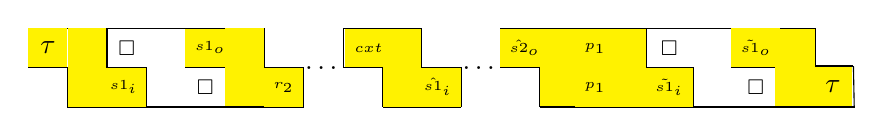
\begin{tikzpicture}
  \draw (0,1) -- (3,1) ;
  \draw (4,1) -- (5,1) ;
  \draw (0.5,0) -- (3.5,0);
  \draw (4.5,0) -- (5.5,0) ;
  \draw (0,1)--(0,0.5) -- (0.5,0.5) -- (0.5,0) -- (1.5,0) ;
  \draw (0.25,0.75)  node[minimum size=0.495cm,fill=yellow] {${ \silent}$};
  \draw (0.75,0.75)  node[minimum size=0.5cm,fill=yellow] {$\ $};
  \draw (0.76,0.25)  node[minimum size=0.5cm,fill=yellow] {$\ $};
  \draw (1.21,0.25)  node[minimum size=0.5cm,fill=yellow] {${\scriptscriptstyle s1_i}$};
  
  \draw (2,1) -- (2,0.5) -- (2.5,0.5) -- (2.5,0) -- (1.5,0)  -- (1.5,0.5) -- (1,0.5) -- (1,1);

 \draw (1.25,0.75) node{$\noact$};%node[minimum size=0.5cm,draw,draw=white] {$\noact$};
 \draw (2.25,0.25) node{$\noact$};
 \draw (2.31,0.75)  node[minimum size=0.47cm,draw,fill=yellow, draw=yellow] {${\scriptscriptstyle s1_o}$};
  \draw (2.75,0.75)  node[minimum size=0.48cm,draw,fill=yellow,yellow] {$\ $};
  \draw (2.75,0.26)  node[minimum size=0.49cm,draw,fill=yellow,yellow] {$\ $};

  \draw (3.245,0.25)  node[minimum size=0.475cm,draw,fill=yellow,draw=yellow] {${\scriptscriptstyle   r_2}$};
  
  \draw (3.75,0.5) node{$\dots$};
  
  \draw(3.5,0.5) -- (3.5,0);
%%     \draw (3.25,0.75)  node[minimum size=0.5cm,draw,draw=white] {$\noact$};
%%  \draw (3.75,0.75)  node[minimum size=0.5cm,draw,white] {$\ $};
%%  \draw (3.75,0.25)  node[minimum size=0.5cm,draw,white] {$\ $};
%%  \draw (4.25,0.25)  node[minimum size=0.5cm,draw,draw=white] {$\noact$};
\draw  (4,1) --  (4,0.5) -- (4.5,0.5) -- (4.5,0)   (3.5,0.5) -- (3,0.5) -- (3,1);
% \draw (3.25,0.75) node{$\noact$};%node[minimum size=0.5cm,draw,draw=white] {$\noact$};
%  \draw (4.25,0.25) node{$\noact$};
\draw (4.75,0.745)  node[minimum size=0.485cm,draw,fill=yellow,yellow] {$\ $};
  \draw (4.38,0.75) node[minimum size=0.47cm,draw,fill=yellow, draw=yellow] 
  {${\scriptscriptstyle  cxt \ }$};
  
  \draw (4.75,0.25)  node[minimum size=0.48cm,draw,fill=yellow,yellow] {$\ $};
  \draw (5.2,0.255)  node[minimum size=0.485cm,draw,fill=yellow,draw=yellow] {${\scriptscriptstyle  \hat{s1}_i}$};
  \draw(5,1) -- (5,0.5) -- (5.5,0.5) -- (5.5,0);
   
   \draw (5.75,0.5) node{$\dots$};
   
    \draw (6,1) -- (10,1) ;
 %   \draw (7,1) -- (7,0.5) -- (7.5,0.5) -- (7.5,0);
    \draw (6.5,0) -- (10.5,0);
    \draw   (6,1)-- (6,0.5) -- (6.5,0.5) -- (6.5,0.5) -- (6.5,0) ;
     \draw (6.75,0.75)  node[minimum size=0.47cm,fill=yellow, draw=yellow] {$\ $};
 \draw (6.36,0.75) node[minimum size=0.475cm,draw,fill=yellow,draw=yellow] 
 {${\scriptscriptstyle \hat{s2}_o \ }$};%node[minimum size=0.5cm,draw,draw=white] {$\noact$};
   \draw (6.75,0.26)  node[minimum size=0.485cm,fill=yellow, draw=yellow] {$\ $};

% \draw (7.20,0.25) node[minimum size=0.475cm,fill=yellow, draw=yellow] {${\scriptscriptstyle{p_1}} \ 
\draw (7.20,0.25)  node[minimum size=0.475cm,draw,fill=yellow,draw=yellow] {${\scriptscriptstyle p_1}$};
\draw (7.2,0.74) node[minimum size=0.48cm,draw,fill=yellow,draw=yellow]{${\scriptscriptstyle p_1}$};
\draw (7.6,0.74)  node[minimum size=0.48cm,draw,fill=yellow, draw=yellow] {$ \ $};
\draw (7.6,0.25)  node[minimum size=0.48cm,draw,fill=yellow, draw=yellow] {$ \ $};
\draw (8.14,0.25)  node[minimum size=0.475cm,draw,fill=yellow,draw=yellow] {${\scriptscriptstyle \tilde{s1}_i}$};
 \draw (8.14,0.75) node{$\noact$};%node[minimum size=0.5cm,draw,draw=white] {$\noact$};
 \draw (9.24,0.25) node{$\noact$};
  \draw (7.85,1) -- (7.85,0.5) ;
   \draw (7.85,0.5) -- (8.45,0.5) ;
      \draw  (8.45,0.5) --(8.45,0) ;
       \draw  (8.93,1) --(8.93,0.5) ;
        \draw  (8.93,0.5) --(9.5,0.5) ;
             \draw  (9.49,0.5) --(9.49,0) ;
         \draw  (9.49,0.5) --(9.49,0) ;
         \draw(10.0,1) -- (10.0,0.5);
          \draw(10,0.52) -- (10.48,0.52);
          \draw(10.48,0.52)--(10.49,0);
%  $};
%
%%     \draw (7.3,0.75)   node{$\noact$};
%%  \draw (7.75,0.75) node{$\ $};
%%  \draw (7.76,0.26) node {$\ $};
%%  \draw (8.25,0.26)  node {$\noact$ };
%
%  \draw (8.3,0.75)  node[minimum size=0.48cm,draw,fill=yellow, draw=yellow] {${\scriptscriptstyle \hat{s2}_o}$};
%  \draw (8,1)--(8,0.5)--(8.5,0.5) -- (8.5,0);
% % \draw(9.5,0.5) --(9.5,0);
%  \draw (8.745,0.75)  node[minimum size=0.48cm,draw,fill=yellow,yellow] {$\ $};
%  \draw (8.75,0.26)  node[minimum size=0.48cm,draw,fill=yellow,yellow] {$\ $};
 %\draw (9.24,0.26)  node[minimum size=0.48cm,draw,fill=yellow,draw=yellow] {${\scriptscriptstyle p_1}$};
 %\draw(9.5,0.5) --(9.5,0);
    % \draw (9,1) -- (10,1) -- (10,0.5) -- (10.5,0.5) --  (10.5,0) -- (9.5,0)  (9.5,0.5) -- (9,0.5) -- (9,1);
 \draw (9.24,0.75) node[minimum size=0.48cm,draw,fill=yellow,draw=yellow]{${\scriptscriptstyle \tilde{s1}_o}$};%node[minimum size=0.5cm,draw,draw=white] {$\noact$};
 
 \draw (10.22,0.26) node [minimum size=0.48cm,draw,fill=yellow,draw=yellow]{$\silent $};
%{${\scriptscriptstyle \tilde{s1}_i}$};
 \draw (9.74,0.745) node [minimum size=0.485cm,draw,fill=yellow,draw=yellow]{$\ $};
 \draw (9.735,0.26) node [minimum size=0.48cm,draw,fill=yellow,draw=yellow]{$\ $};
 %  \draw (10.8,0.5) node{$\dots$};
% \draw (10,1) -- (10,0.5) -- (10.5,0.5)--(10.5,0);
  %\draw (10.31,0.75)  node{$\noact$};
%  \draw (10.75,0.75)  node {$\ $};
%  \draw (10.75,0.26)  node{$\ $};
% \draw (11.25,0.25)  node {$\noact$};
%   \draw (11,1) -- (11,0.5) -- (11.5,0.5) -- (11.5,0);% -- (10,0) -- (9,0) -- (9,0.5) -- (8.5,0.5) -- (8.5,1);
%    \draw (11,1) -- (11.5,1) -- (12,1) -- (12,0.5) -- (12.5,0.5)--(12.5,0)--(11.5,0);
   %\draw (11.25,0.25)  node[minimum size=0.48cm,draw,fill=yellow,draw=yellow] {$\noact$};
%    \draw (11.31,0.75) node[minimum size=0.48cm,draw,fill=yellow,draw=yellow]{${\scriptscriptstyle \tilde{s1}_o}$};
%    \draw (11.75,0.26)node[minimum size=0.48cm,draw,fill=yellow,draw=yellow]{$\ $};
%      \draw (11.75,0.75)node[minimum size=0.48cm,draw,fill=yellow,draw=yellow]{$\ $};
%     \draw (12.2,0.25) node[minimum size=0.478cm,draw,fill=yellow,draw=yellow]{\;$\silent$\;  };
  \end{tikzpicture}
  \caption{The link chain structure arising from reactions and context processes.}
   \label{fig:backbone}
 \end{figure}
 \end{example}
}

Example~\ref{ex:backbone}   outlines two different roles of the processes defining the translation of an interactive process: those processes encoding the reactions and the context provide the backbone of each transition, whereas the processes encoding the entities provide the resources needed for the communication to take place.
 
With the next proposition, we analyse the structure of a c\CNA \ 
process encoding of  a reactive process after one step transition.
In the following four statements, for brevity, we let ${\cal A} = (S, A)$ be a RS, and let  $\pi=(\gamma,\delta)$ be an extended interactive process in $A$, with $\gamma=\{C_i\}_{i\in\mathbb{N}}$ and $\delta=\{D_i\}_{i\in\mathbb{N}}$. Moreover, we denote by $\pi^j$ the shift of $\pi$ starting at the $j$-th state sequence; formally we let $\pi^j=(\gamma^j,\delta^j)$ with
$\gamma^j=\{C_i'\}_{i\in\mathbb{N}}$, $\delta^j=\{D_i'\}_{i\in\mathbb{N}}$ with 
  $C_0'=C_j \cup D_j$, $D'_0 = \emptyset$, and   $C_i'=C_{i+j}$, $D_i'= D_{i+j}$ for any $i\geq 1$.

 \begin{restatable}[Correctness 1]{proposition}{propcorruno}
% \begin{proposition}(correctness 1)\\
 \label{prop:corr1}
% We define $\pi' = (\gamma',\delta')$ with $\gamma' = C_0',\dots,C_{n-1}'$ and $\delta' = D_0',\dots,D_{n-1}'$ as $C_0' = C_1 \cup D_1$,  and
% $C_i' = C_{i+1}$, $D_{i}' = D_{i+1}$ with $ 1 \leq i < n$.
 Let 
 $P=\llbracket{\cal A},\gamma\rrbracket$ with
$$P  = \restrict{\mathit{names}} (\Pi_{a \in A}P_a ~|~ \mathit{Cxt}^1 ~|~ \Pi_{s \in C_0}P_s ~|~ \Pi_{s \notin C_0}\overline{P}_s).
$$
 If there exists  $P'$  such that $P \xrightarrow{v}P'$,  it holds that:
 \begin{enumerate}
 \item
  $v=\link{\silent}{\silent}\dots\link{\silent}{\silent}$, and
  \item 
 $P'= \restrict{\mathit{names}} (Init | \Pi_{a \in A}P_a~|~ \mathit{Cxt}^2 ~|~ \Pi_{s \in C_1 \cup D_1}P_s| \Pi_{s \notin C_1 \cup D_1}\overline{P}_s)$.
 \end{enumerate}
Moreover, given $\pi^1=(\gamma^1,\delta^1)$, we have $P' = \llbracket {\cal A},\gamma^1\rrbracket$.
 %\end{proposition}
\end{restatable}
 
% \begin{lemma}[correctness 1 {\color{red} Ma serve ??}]
% \label{cor:complet1}
% Let ${\cal A} = (S, A)$ be a rs, and let  $\pi=(\gamma,\delta)$ be an extended interactive process in $A$, with
% $\gamma = C_0,\dots,C_t$, $\delta = D_0,\dots,D_t$, with $n \geq 0$. Let   $P=[|{\cal A},\gamma|]$ be  its c\CNA~translation. We define $\pi' = (\gamma',\delta')$ with $\gamma' = C_0',\dots,C_{n-1}'$ and $\delta' = D_0',\dots,D_{n-1}'$ as $C_0' = C_1 \cup D_1$,  and
% $C_i' = C_{i+1}$, $D_{i}' = D_{i+1}$ with $ 1 \leq i < n$. Then,
% if $\exists$ $P'$, $P''$ such that $P \xrightarrow{\link{\silent}{\silent}} P'$ and $P \xrightarrow{\link{\silent}{\silent}} P''$, then $P' = P''$.
%\end{lemma}

 
 
% \begin{proposition}[correctness2]
% \label{prop:correctness1}
% Let $P$ be a c\CNA \ process such that $\exists$ a $rs$ ${\cal A}$ and a $n$-step interactive process $\pi=(\gamma,\delta)$ with $\gamma =C_0,\dots,C_n$ and $\delta = D_0,\dots,D_n$ such that $P= [|{\cal A},\gamma|]$. 
% %We set $\pi'=(\gamma',\delta')$ with $\gamma'=C_0',\dots,C_{n-1}'$,  $\delta'=D_0',\dots,D_{n-1}$,  where $C_0'= C_1 \cup D_1$, $C_i'= C_{i+1}$, $D_i=D_{i+1}'$,  and $1 \leq i < n$.
%Then,   $\exists$ $P'$ and $\pi'=(\gamma',\delta')$ such that $P \xrightarrow{\link{\silent}{\silent}}P'$, $P' =[|{\cal A},\gamma'|]$.
% \end{proposition} 
\noindent
Now, we extend the previous result to a series of transitions.
 
 \begin{restatable}[Correctness 2]{corollary}{corrcorrdue} 
% \begin{corollary}[correcteness2]
 \label{corr:corr2}
  Let $P = \llbracket{\cal A},\gamma\rrbracket$ and $j\geq 1$.
%  Let $P$ a  c\CNA process such that exists a rs ${\cal A}$ and an extended  interactive process $\pi=(\gamma,\delta)$ with $\gamma =C_0,\dots,C_t$, $\delta = D_0,\dots,D_t$, with $t \geq 0$, such that $P= [|{\cal A},\gamma|]$. 
If there exists  $P''$ such that $P \xrightarrow{\link{\silent}{\silent}\dots \link{\silent}{\silent}}^{j}P''$, then letting  $\pi^j=(\gamma^j,\delta^j)$ we have
$P'' =\llbracket{\cal A},\gamma^j\rrbracket$.
%such that $P=[|{\cal A}|]$, then if $P \rightarrow^* P'$, then $\exists$ ${\cal A'}$ such that ${\cal A}$  evolves in ${\cal A'}$ and $P'=[|{\cal A'}|]$.
 \end{restatable}


With the following propositions, we prove that, given a RS ${\cal A} = (S, A)$ and an extended  interactive process $\pi=(\gamma,\delta)$, then the $c\CNA$ process $\llbracket{\cal A},\gamma\rrbracket$ can simulate all the evolutions  of $\pi$. 

 \begin{restatable}[Completeness 1]{proposition}{propcompluno} 
% \begin{corollary}[correcteness2]
 \label{prop:compl1}
% \begin{proposition}[completeness1]
 %\label{lem:compl2}
Let   $P=\llbracket{\cal A},\gamma\rrbracket$ and $\pi^1 = (\gamma^1,\delta^1)$.
% be the extended interactive process starting  at the next state sequence. 
Then, 
 % following holds:
 %\begin{enumerate} 
 %\item  
  $P \xrightarrow{\link{\silent}{\silent}\dots \link{\silent}{\silent}} P'=\llbracket{\cal A},\gamma^1\rrbracket$.
 %\item if $\exists$ $P'$, $P''$ such that $P \xrightarrow{\link{\silent}{\silent}} P'$ and $P \xrightarrow{\link{\silent}{\silent}} P''$, then $P' = P''$.
 %\end{enumerate}
% \end{proposition} 
\end{restatable}

\noindent
Now, we extend the previous result to a series of transitions.
 
\begin{restatable}[Completeness 2]{corollary}{corrcompldue} 
% \begin{corollary}[correcteness2]
 \label{corr:compl2}
% \begin{corollary}[completeness2]
 %\label{prop:completeness}
Let $P=\llbracket{\cal A},\gamma\rrbracket$ and  $\pi^j= (\gamma^j,\delta^j)$.  
Then, $P \xrightarrow{\link{\silent}{\silent}\dots\link{\silent}{\silent}}^j P''=\llbracket{\cal A},\gamma^j\rrbracket$.  
 \end{restatable}

 
% 
% \begin{proposition}[correctness]
% Let $P$ a c\CNA\  process such that exists a reaction system ${\cal A}$ such that $P=[|{\cal A}|]$, then if $P \rightarrow P'$, then $\exists$ ${\cal A'}$ such that ${\cal A}$  evolves in ${\cal A'}$ in one step and $P'=[|{\cal A'}|]$.
% \end{proposition}
 
  
%% !TEX root = ./main_RS2L_LNCS.tex
\section{Example: \emph{lac} operon}
\label{ex:lactose}
In this section we present the encoding of a RS example
taken from~\cite{CMMBM12}.
%, concerning the lac Operon.
\subsection{The \emph{lac} operon}
An operon is a cluster of genes under the control of a single promoter. 
The \emph{lac} operon  is involved in the metabolism of lactose in \emph{Escherichia coli} cells;
it is composed by three adjacent structural genes (plus some regulatory components):  $lacZ$, $lacY$ and $lacA$ encoding for two enzymes $Z$ and $A$, and a transporter $Y$, involved in the digestion of the $lactose$. The main regulations are:
\begin{itemize}
\item 
%\begin{color}{red}
the gene $lacI$ encodes a repressor protein $I$;
%\end{color}
\item the DNA sequence, called \emph{promoter},  is recognised by a RNA polymerase
to iniziate the transcription  of the genes $lacZ$, $lacY$ and $lacA$;
\item a DNA segment, called  the \emph{operator} ($OP$),   obstructs the RNA polymerase functionality when  the repressor protein $I$ is bound to it forming $I\textrm{-}OP$;
\item  a short DNA sequence, called the $CAP\textrm{-}binding\ site$, when it is bound to the complex composed by  the protein $CAP$ and the signal molecule $cAMP$, acts as a promoter for the interaction between the RNA polymerase and the promoter.
\end{itemize}
The functionality of the \emph{lac} operon depends on the integration of two control mechanisms, one mediated by \emph{lactose}, and the other one mediated by \emph{glucose}. 

In the first control mechanism, an effect of the absence of the \emph{lactose} is that $I$ is able to bind the operator sequence preventing the \emph{lac} operon expression. If lactose is available, $I$ is unable to bind the operator sequence, and the \emph{lac} operon can be potentially expressed.

In  the second control mechanism, when glucose is absent, the molecule $cAMP$ and the protein $CAP$ increase the \emph{lac} operon expression, thanks to the fact that  the binding between the molecular complex $cAMP\textrm{-}CAP$ and the $CAP\textrm{-}binding\ site$ increases.
In summary, the condition promoting the operon
gene expression is when the $lactose$ is present and the $glucose$ is absent.

In the following we report the description of the \emph{lac} operon mechanism in the reaction system formalism
and then show its encoding in c\CNA. 

\subsection{The RS formalization}\label{subsec:RSlacoperon}
The reaction system for the \emph{lac} operon is defined as
$A_{lac} = (S, A)$, where the set S represents
the main biochemical components involved in this genetic system, while the reaction set A contains the biochemical
reactions involved in the regulation of the \emph{lac} operon expression. Formally, the \emph{lac} operon reaction system is defined as
follows:
$S$ is the set
{\small
$$\{lac, Z, Y, A, lacI, I, I\textrm{-}OP, cya, cAMP, crp, CAP,cAMP\textrm{-}CAP, lactose,glucose\},$$
}
and A consists of the following 10 reactions:
{\small
\[
\begin{array}{lcllcl}
a_1 &= &(\{lac\},\{. . .\},\{lac\}), & a_6 &= &(\{cya\},\{. . .\},\{cAMP\}),\\
a_2 &= &(\{lacI\},\{. . .\},\{lacI\}), & a_7 &= &(\{crp\},\{. . .\},\{crp\}),\\
a_3 &= &(\{lacI\},\{. . .\},\{I\}), & a_8 &= &(\{crp\},\{. . .\},\{CAP\}),\\
a_4 &= &(\{I\},\{lactose\},\{I\textrm{-}OP\}), & a_9 &= &(\{cAMP, CAP\},\{glucose\},\{cAMP\textrm{-}CAP\}),\\
a_5 &= &(\{cya\},\{. . .\},\{cya\}),&
a_{10} &=& (\{lac, cAMP\textrm{-}CAP\},\{I\textrm{-}OP\},\{Z, Y, A\}).
\end{array}
\]
}
The default context ($DC$) is composed by those entities that are always present in the system
$DC = \{lac,lacI,I,cya,cAMP,crp,CAP\}$, whereas the $lactose$ and the $glucose$ are given non-deterministically by the context.
\subsection{The RS encoding}
For the sake of readability, the encoding we propose exploits the specific features of the example in hand 
to perform some simplifications:
\begin{itemize}
\item for the entities in the default context, $s \in DC$, as they are persistent, we do not provide the $\overline{P_s}$ processes and the $Cxt_s$ processes;
\item for the reactions requiring the presence of entities $s \in DC$, we do not provide the reaction alternative behaviour when $s$ is absent;
\item the $Cxt_s$ processes are specified only for those entitiess that are really provided by the context.
\end{itemize}
Moreover, we do not model the \emph{dummy} entity that is specified by  dots ($\dots$) by the RS reactions in Section~\ref{subsec:RSlacoperon}.
Finally, we exclude the \emph{duplication reactions} ($a_1$, $a_2$, $a_5$, $a_7$), and renumber the remaining reactions :
{\small
\[
\begin{array}{cccl}
%a1 &= &(\{lac\},\{. . .\},\{lac\}),\\
%a2 &= &(\{lacI\},\{. . .\},\{lacI\}),\\
\textrm{old } &\textrm{new }&& \textrm{reactions}\\
a_3 &a_1&=&(\{lacI\},\{. . .\},\{I\}),\\
a_4 &a_2&=&(\{I\},\{lactose\},\{I\textrm{-}OP\}),\\
%a5 &= &(\{cya\},\{. . .\},\{cya\}),\\
a_6 & a_3&=&(\{cya\},\{. . .\},\{cAMP\}),\\
%a7 &= &(\{crp\},\{. . .\},\{crp\}),\\
a_8 &a_4&=&(\{crp\},\{. . .\},\{CAP\}),\\
a_9 &a_5&=&(\{cAMP, CAP\},\{glucose\},\{cAMP\textrm{-}CAP\}),\\
a_{10} & a_6&=& (\{lac, cAMP\textrm{-}CAP\},\{I\textrm{-}OP\},\{Z, Y, A\}).
\end{array}
\]
}
%\paragraph{Duplication reactions.}
%As explained previously, their encoding is omitted.
%%$
%\begin{array}{lcccl}
%P_{ai} & \defeq& P_d(ai,s) & = & \startchain{r_i}\chainedlink{s_i}{\noact}\chainedlink{\noact}{s_o}
%\chainedlink{\tilde{s}_i}{\noact}\chainedlink{\noact}{\tilde{s}_o}\chainend{r_{i+1}}.P_d(ai,s)
%\end{array}
%$,
%with $r_1 = \silent$.
%There are four duplication rules:\\ $P_d(a1,lac)$, $P_d(a2,lacI)$,$P_d(a5,cya)$,$P_d(a7,crp)$.\\
\paragraph{Expression reactions.}
First we define the parametric process
\[
\begin{array}{lcl}
% P_i(s1,s2) & \defeq & \startchain{r_i}\chainedlink{s1_i}{\noact}\chainedlink{\noact}{s1_o}
%\chainedlink{\tilde{s2}_i}{\noact}\chainedlink{\noact}{\tilde{s2}_o}\chainend{r_{i+1}}.P_i(s1,s2)\\
 P_i(s1,s2) & \defeq & \startchain{r_i}\chainedlink{s1_i}{\noact}\chainedlink{\noact}{s1_o}
 \chainedlink{r_{i+1}}{\noact}\chainedlink{\noact}{p_{i}}\chainedlink{\tilde{s2}_i}{\noact}
\chainedlink{\noact}{\tilde{s2}_o}\chainend{p_{i+1}}.P_i(s1,s2)\\
\end{array}
\]
Then, we let $P_{a1}\defeq P_1(lacI,I)$,  $P_{a3} \defeq P_3(cya,cAMP)$, and $P_{a4} \defeq P_4(crp,CAP)$.
%\[
%\begin{array}{lcl}
%P_{a1} & =& \startchain{\silent}\chainedlink{lac_i}{\noact}\chainedlink{\noact}{lac_o}\chainedlink{\tilde{lac}_i}{\noact}\chainedlink{\noact}{\tilde{lac}_o}\chainend{r_2}.P_{a1}\\
%P_{a2} & =& \startchain{r_2}\chainedlink{lacI_i}{\noact}\chainedlink{\noact}{lacI_o}\chainedlink{\tilde{lacI}_i}{\noact}\chainedlink{\noact}{\tilde{lacI}_o}\chainend{r_3}.P_{a2}\\
%P_{a3} & =& \startchain{r_3}\chainedlink{I_i}{\noact}\chainedlink{\noact}{I_o}\chainedlink{\tilde{I}_i}{\noact}\chainedlink{\noact}{\tilde{I}_o}\chainend{r_4}.P_{a3}\\
\paragraph{Regulation reactions.}

{\small
\[
\begin{array}{lcl}
%P_{a2} & \defeq& \startchain{r_2}\chainedlink{I_i}{\noact}\chainedlink{\noact}{I_o}\chainedlink{\overline{lactose}_i}{\noact}\chainedlink{\noact}{\overline{lactose}_o}
%\chainedlink{\widetilde{I\textrm{-}OP}_i}{\noact}\chainedlink{\noact}{\widetilde{I\textrm{-}OP}_o}\chainend{r_3}.P_{a2}  \\
P_{a2} & \defeq& \startchain{r_2}\chainedlink{I_i}{\noact}\chainedlink{\noact}{I_o}\chainedlink{\overline{lactose}_i}{\noact}\chainedlink{\noact}{\overline{lactose}_o}
\chainedlink{r_3}{\noact}\chainedlink{\noact}{p_2}
\chainedlink{\widetilde{I\textrm{-}OP}_i}{\noact}\chainedlink{\noact}{\widetilde{I\textrm{-}OP}_o}\chainend{p_3}.P_{a2}  \\
&&+\\
 && \startchain{r_2}\chainedlink{lactose_i}{\noact}\chainedlink{\noact}{lactose_o}\chainedlink{r_3}{\noact}\chainedlink{\noact}{p_2}\chainend{p_3}.P_{a2} \ +\  \startchain{r_2}\chainedlink{\overline{I}_i}{\noact}\chainedlink{\noact}{\overline{I}_o}\chainedlink{r_3}{\noact}\chainedlink{\noact}{p_2}\chainend{p_3}.P_{a2}\\[5pt]
 \\
%%P_{a5} & =& \startchain{r_5}\chainedlink{cya_i}{\noact}\chainedlink{\noact}{cya_o}\chainedlink{\tilde{cya}_i}{\noact}\chainedlink{\noact}{\tilde{cya}_o}\chainend{r_6}.P_{a5}\\
%P_{a6} & =& \startchain{r_6}\chainedlink{cya_i}{\noact}\chainedlink{\noact}{cya_o}\chainedlink{\tilde{cya}_i}{\noact}\chainedlink{\noact}{\tilde{cya}_o}\chainend{r_7}.P_{a6}\\
%%P_{a7} & =& \startchain{r_7}\chainedlink{crp_i}{\noact}\chainedlink{\noact}{crp_o}\chainedlink{\tilde{crp}_i}{\noact}\chainedlink{\noact}{\tilde{crp}_o}\chainend{r_8}.P_{a7}\\
%P_{a8} & =& \startchain{r_8}\chainedlink{crp_i}{\noact}\chainedlink{\noact}{crp_o}\chainedlink{\tilde{CAP}_i}{\noact}\chainedlink{\noact}{\tilde{CAP}_o}\chainend{r_9}.P_{a8}\\
P_{a5} & \defeq& \startchain{r_5}\chainedlink{cAMP_i}{\noact}\chainedlink{\noact}{cAMP_o}
\chainedlink{CAP_i}{\noact}\chainedlink{\noact}{CAP_o}\chainedlink{\overline{glucose}_i}{\noact}
\chainedlink{\noact}{\overline{glucose}_o}\chainedlink{r_6}{\noact}
\chainedlink{\noact}{p_5}
\chainedlink{\widetilde{cAMP\textrm{-}CAP}_i}{\noact}\chainedlink{\noact}{\widetilde{cAMP\textrm{-}CAP}_o}
\chainend{p_6}.P_{a5}\\
%P_{a5} & \defeq& \startchain{r_5}\chainedlink{cAMP_i}{\noact}\chainedlink{\noact}{cAMP_o}
%\chainedlink{CAP_i}{\noact}\chainedlink{\noact}{CAP_o}\chainedlink{\overline{glucose}_i}{\noact}
%\chainedlink{\noact}{\overline{glucose}_o}
%\chainedlink{\widetilde{cAMP\textrm{-}CAP}_i}{\noact}\chainedlink{\noact}{\widetilde{cAMP\textrm{-}CAP}_o}
%\chainend{r_6}.P_{a5}\\
&& +\\
&& \startchain{r_5}\chainedlink{glucose_i}{\noact}\chainedlink{\noact}{glucose_o} \chainedlink{r_6}{\noact}\chainedlink{\noact}{p_5}\chainend{p_6}.P_{a5}\\
&& + \\
&&  \startchain{r_5}\chainedlink{\overline{cAMP}_i}{\noact}\chainedlink{\noact}{\overline{cAMP}_o} \chainedlink{r_6}{\noact}\chainedlink{\noact}{p_5}\chainend{p_6}.P_{a5} \ + \ \startchain{r_5}\chainedlink{\overline{CAP}_i}{\noact}\chainedlink{\noact}{\overline{CAP}_o} \chainedlink{r_6}{\noact}\chainedlink{\noact}{p_5}\chainend{p_6}.P_{a5}\\[5pt]
\\
%\end{array}
%\]\\
%%$lac$ operon expression.\\
%$
%\begin{array}{lcl}
P_{a6} & \defeq& \startchain{r_{6}}\chainedlink{lac_i}{\noact}\chainedlink{\noact}{lac_o}
\chainedlink{cAMP\textrm{-}CAP_i}{\noact}\chainedlink{\noact}{cAMP\textrm{-}CAP_o}\chainedlink{\overline{I\textrm{-}OP}_i}{\noact}
\chainedlink{\noact}{\overline{I\textrm{-}OP}_o}\chainedlink{cxt_1}{\noact}
\chainedlink{\noact}{p_6}
\chainedlink{\tilde{z}_i}{\noact}\chainedlink{\noact}{\tilde{z}_o}
\chainedlink{\tilde{y}_i}{\noact}\chainedlink{\noact}{\tilde{y}_o}
\chainedlink{\tilde{A}_i}{\noact}\chainedlink{\noact}{\tilde{A}_o}
\chainend{\silent}.P_{a6}\\
%P_{a6} & \defeq& \startchain{r_{6}}\chainedlink{lac_i}{\noact}\chainedlink{\noact}{lac_o}
%\chainedlink{cAMP_i}{\noact}\chainedlink{\noact}{cAMP_o}\chainedlink{\overline{I\textrm{-}OP}_i}{\noact}
%\chainedlink{\noact}{\overline{I\textrm{-}OP}_o}
%\chainedlink{\tilde{z}_i}{\noact}\chainedlink{\noact}{\tilde{z}_o}
%\chainedlink{\tilde{y}_i}{\noact}\chainedlink{\noact}{\tilde{y}_o}
%\chainedlink{\tilde{A}_i}{\noact}\chainedlink{\noact}{\tilde{A}_o}
%\chainend{cxt_1}.P_{a6}\\
&& +\\
&& \startchain{r_{6}}\chainedlink{I\textrm{-}OP_i}{\noact}\chainedlink{\noact}{I\textrm{-}OP_o} \chainedlink{cxt_1}{\noact}\chainedlink{\noact}{p_6}\chainend{\silent}.P_{a6} \\
&& + \\
&&  \startchain{r_{6}}\chainedlink{\overline{lac}_i}{\noact}\chainedlink{\noact}{\overline{lac}_o} \chainedlink{cxt_1}{\noact}\chainedlink{\noact}{p_6}\chainend{\silent}.P_{a6} \ + \ \chainedlink{\overline{cAMP\textrm{-}CAP}_i}{\noact}\chainedlink{\noact}{\overline{cAMP\textrm{-}CAP}_o} \chainedlink{cxt_1}{\noact}\chainedlink{\noact}{p_6}\chainend{\silent}.P_{a6}
\end{array}
\]
}
\paragraph{Processes for the entities.}
We exploit the specificity of the example in hand to optimise the code, and we specify exactly
the number of solid links that each process encoding an entity must offer.
For the always present entities  we let:
%{\color{red} For the always present entities we define the parametric process $P(s)\defeq \link{s_i}{s_o}.P_{s}$, and we let:
%\[
%\begin{array}{lcl@{\qquad}lcl@{\qquad}lcl@{\qquad}lcl}
%P_{cya}&\defeq&P(cya) &P_{crp}&\defeq&P(crp)&P_{lacI}&\defeq&P(lacI) &
% P_{lac}&\defeq&P(lac)
%\end{array}\]
\[
\begin{array}{lcl@{\qquad}lcl}
P_{cya}&\defeq&\link{cya_i}{cya_o}.P_{cya} &
P_{crp}&\defeq&\link{crp_i}{crp_o}.P_{crp}\\[5pt]
P_{lacI}&\defeq& \link{lacI_i}{lacI_o}.P_{lacI} &
 P_{lac}&\defeq&\link{lac_i}{lac_o}.P_{lac}
\end{array}\]
For the entities always produced (i.e. not present only at the first step), we  provide a  parametric
definition  
$P_e(s) \defeq  \startchain{s_i}\chainedlink{s_o}{\noact}\chainedlink{\noact}{\tilde{s}_i}\chainend{\tilde{s}_o}.P_e(s) +  \startchain{\tilde{s_i}}\chainend{\tilde{s}_o} .P_e(s) $.\\
% There are four entities of the first type: $P_d(lac)$, $P_d(cya)$, $P_d(crp)$, $P_d(lacI)$.
 There are three entities of the second type:  $$P_{cAMP}\defeq P_e(cAMP) \qquad P_{CAP} \defeq P_e(CAP)\qquad P_I \defeq P_e(I).$$


The entity $I\textrm{-}OP$ can be either produced (by $a_2$) or tested for absence (by $a_6$).
Correspondingly, the process  $P_{I\textrm{-}OP}$ is defined as follows:
\[\begin{array}{lcl}
P_{I\textrm{-}OP}&\defeq & 
\sum_{h=0}^1 (\startchain{I\textrm{-}OP_i}\chainedlink{I\textrm{-}OP_o}{\noact}\chainend{\noact})^h  \, \startchain{\widetilde{I\textrm{-}OP}_i}\chainend{\widetilde{I\textrm{-}OP}_o}.P_{I\textrm{-}OP}
%\\
%&&+\\
%&&\sum_{h=0}^1(\startchain{I-OP_i}\chainedlink{I-OP_o}{\noact}\chainend{\noact})^h\ \startchain{\widetilde{I-OP}_i}\chainedlink{\widetilde{I-OP}_o}{\noact}\chainedlink{\noact}{\underline{I-OP}_i}\chainend{\underline{I-OP}_o}.P_{I-OP}\\
%&&
\  +\ %\\
%&&
\link{I\textrm{-}OP_i}{I\textrm{-}OP_o}.\overline{P_{I\textrm{-}OP}}\\
\overline{P_{I\textrm{-}OP}} & \defeq & 
% P_{I\textrm{-}OP}(\overline{I\textrm{-}OP})\\
\sum_{h=0}^1  (\startchain{\overline{I\textrm{-}OP}_i}\chainedlink{\overline{I\textrm{-}OP}_o}{\noact}\chainend{\noact})^h \,
\startchain{\widetilde{I\textrm{-}OP}_i}\chainend{\widetilde{I\textrm{-}OP}_o}.P_{I\textrm{-}OP}%\\
%&&
\ +\ %\\
%&&
\link{\overline{I\textrm{-}OP}_i}{\overline{I\textrm{-}OP}_o}.\overline{P_{I\textrm{-}OP}}\\

\end{array}
\]
\noindent
The  process $P_{cAMP\textrm{-}CAP}$ is similar to $P_{I\textrm{-}OP}$, as it is produced by $a_5$ and tested for presence by $a_6$. 
Its code is omitted.
%Its code is  in Table~\ref{tab:cAMP-CAP}, in the Appendix.

The $lactose$ is provided by the context and tested for absence by $a_2$.

\[
\begin{array}{lcllcl}
P_{lactose} &\defeq &%== \overline{P_{glucose}}&\defeq & P_{glu-lact}(\overline{glucose})\\
\sum_{h=0}^1 (\startchain{lactose_i}\chainedlink{lactose_o}{\noact}\chainend{\noact})^h\ \link{\widehat{lactose_i}}{\widehat{lactose_o}}.P_{lactose}
\\
&& + \\
&& \sum_{h=0}^1 (\startchain{lactose_i}\chainedlink{lactose_o}{\noact}\chainend{\noact})^h\ \link{\underline{lactose_i}}{\underline{lactose_o}}.\overline{P_{lactose}}\\
\\
\overline{P_{lactose}} &\defeq &\sum_{h=0}^1 (\startchain{\overline{lactose}_i}\chainedlink{\overline{lactose}_o}{\noact}\chainend{\noact})^h\ \link{\widehat{lactose_i}}{\widehat{lactose_o}}.P_{lactose}\\
&&+\\
&& \sum_{h=0}^1 (\startchain{\overline{lactose}_i}\chainedlink{\overline{lactose}_o}{\noact}\chainend{\noact})^h\ \link{\underline{lactose_i}}{\underline{lactose_o}}.\overline{P_{lactose}}\\
\end{array}
\]
\noindent
The  process $P_{glucose}$ is similar to $P_{lactose}$ and tested for absence by $a_5$. 
Its code is omitted.
%Its code is  in Table~\ref{tab:glucose}, in the Appendix.

The entity $z$ can only be produced by rule $a_6$, while it is never provided by the context. Moreover, there is no rule for testing its presence or absence.
\[
\begin{array}{lcl@{\qquad\qquad}lcl}
P_z&\defeq &\startchain{\tilde{z_i}}\chainedlink{\tilde{z_o}}{\noact}\chainedlink{\noact}{\underline{z_i}}\chainend{\underline{z_o}}.P_z\ + \
\link{\underline{z_i}}{\underline{z_o}}.\overline{P_z}
&
\overline{P_z} &\defeq &\startchain{\tilde{z_i}}\chainedlink{\tilde{z_o}}{\noact}\chainedlink{\noact}{\underline{z_i}}\chainend{\underline{z_o}}.\overline{P_z}\ + \
\link{\underline{z_i}}{\underline{z_o}}.\overline{P_z}\\\end{array}
\]
\noindent
The entities $y$ and $A$ are treated likewise $z$. Their processes are omitted.
%in Table~\ref{tab:yA} in the Appendix.



\paragraph{Context.}
%Now, we define the behaviour of the context.
The entities in $DC$ are assumed always present by default, so no context process is needed for them.
The entities $z$, $y$, and $A$ are assumed never provided by the context:
% Their processes are
\[
\begin{array}{rcl@{\qquad}rcl}
Cxt_{z}&\defeq & \startchain{cxt_1}\chainedlink{\underline{z}_i}{\noact}\chainedlink{\noact}{\underline{z}_o}\chainend{cxt_2}.Cxt_{z}
&
Cxt_{y}&\defeq & \startchain{cxt_2}\chainedlink{\underline{y}_i}{\noact}\chainedlink{\noact}{\underline{y}_o}\chainend{cxt_3}.Cxt_{y}
\\
Cxt_{A}&\defeq & \startchain{cxt_3}\chainedlink{\underline{A}_i}{\noact}\chainedlink{\noact}{\underline{A}_o}\chainend{cxt_4}.Cxt_{A} 
\end{array}
\]
 Also, for the sake of presentation, we assume that the $glucose$ is never provided and $lactose$ is always provided by the context:
\[
\begin{array}{lcl}
Cxt_{lactose}&\defeq& \startchain{cxt_4}\chainedlink{\widehat{lactose}_i}{\noact}\chainedlink{\noact}{\widehat{lactose}_o}\chainend{cxt_5}.Cxt_{lactose}\\
Cxt_{glucose}&\defeq & \startchain{cxt_5}\chainedlink{\underline{glucose}_i}{\noact}\chainedlink{\noact}{\underline{glucose}_o}\chainend{p_1}.Cxt_{glucose}
\end{array}
\]

\noindent
%For the sake of presentation, we assume that the $lactose$ is always provided by the context, in contrast,
%$glucose$ is never provided.
%\[
%\begin{array}{lcllcl}
%Cxt_{lactose}&\defeq& \startchain{cxt_4}\chainedlink{\widehat{lactose}_i}{\noact}\chainedlink{\noact}{\widehat{lactose}_o}\chainend{cxt_5}.Cxt_{lactose}
%\\
%Cxt_{glucose}&\defeq & \startchain{cxt_5}\chainedlink{\underline{glucose}_i}{\noact}\chainedlink{\noact}{\underline{glucose}_o}\chainend{p_1}.Cxt_{glucose}
%\end{array}
%\]
\noindent
In the following we let $CXT \defeq Cxt_z | Cxt_y |Cxt_A | Cxt_{lactose} | Cxt_{glucose}$ be the processes for context. 
%
The whole system
%, encoding an extended interactive process, with the previous context behaviour
is as follows: 
\[ lacOp \defeq \restrict{names} (\Pi_{i=1}^6 P_{ai} | \Pi_{s \in DC} P_s |   \Pi_{s \in S \backslash DC} \overline{P}_s| CXT)
\]

\paragraph{Execution.}
Now, we show  the execution of two transitions. 
After the first transition, the entity $cAMP\textrm{-}CAP$ is produced due to the absence of  $glucose$(see $P_{a5}$), while the presence of $lactose$ inhibits the production of $I\textrm{-}OP$ (see $P_{a2}$): $lacOp \xrightarrow{\restrict{names} v} lacOp'$,
where
{\small
$$
\begin{array}{rcl}
v & = & \link{\silent}{lac_i}\dots \link{lactose_o}{r3}\dots
 \link{r_5}{cAMP_i}\dots
  \link{\overline{glucose}_o}{r_6}
\dots \link{p_5}{\widetilde{cAMP\textrm{-}CAP}_i}\dots \link{p_6}{\silent}\\[5pt]
%{\underline{glucose}_o}
lacOp' & \defeq & \restrict{names} (\Pi_{i =1}^6 P_{ai} | \Pi_{s \in AP} P_s |   \Pi_{s \in S \backslash AP} \overline{P}_s| CXT)
\end{array}
$$ 
}
with $AP= DC\cup \{cAMP\textrm{-}CAP\}$  the actual context.\\
After the second step the entities $z$, $y$ and $A$ are produced, due to the presence of $cAMP\textrm{-}CAP$ and the absence of $I\textrm{-}OP$ (see $P_{a6}$), thus
$lacOp' \xrightarrow{\restrict{names}v'} lacOp''$
where:
{\small
$$
\begin{array}{rcl}
v' & = & \link{\silent}{lac_i}\dots \link{lac_o}{cAMP-CAP_i}\dots \startchain{\overline{I-OP}_o}
\chainedlink{cxt_1}{\dots}\startchain{\underline{glucose}_o}\chainedlink{p_1}{p_1}
\chainedlink{\dots}{p_6}\chainedlink{\tilde{z}_i}{\tilde{z}_i}\chainedlink{\tilde{z}_o}{\tilde{z}_o}
\chainedlink{\tilde{y}_i}{\tilde{y}_i}\chainedlink{\tilde{y}_o}{\tilde{y}_o}\chainedlink{\tilde{A}_i}{\tilde{A}_i}\chainedlink{\tilde{A}_o}{\tilde{A}_o}\chainend{\silent}\\
%\chainend{cxt_1}\dots \link{\underline{glucose}_o}{\silent}\\[5pt]
lacOp'' & \defeq & \restrict{names} (\Pi_{i =1}^{6} P_{ai} | \Pi_{s \in AP'} P_s |   \Pi_{s \in S \backslash AP'} \overline{P}_s| CXT)
\end{array}
$$
}
with $AP'= DC\cup \{z,y,A\} $.



% !TEX root = ./main_TCS.tex
\section{Examples}
\label{ex:examples}
Semantically, the topmost restriction $\restrict{\mathit{names}}$ filters out any interaction with  virtual links, and releases a private interaction among all participants where all the channel names in the transition labels are hidden (their occurrences are all replaced by $\silent$).
%Hereafter, we shall often omit topmost restrictions
This amounts to require that only complete chains are computed by the interaction.
In this section, for simplicity,  we shall often omit topmost restrictions $\restrict{\mathit{names}}$ from our encoding, but 
 we shall take into account only transitions whose labels are complete chains, i.e. they do not contain 
virtual links and start/end with the $\silent$ action symbol.
This way it is possible to observe all channel names that occur in the interaction.

\subsection{Labelled transition system}
This example is inspired by the example in~\cite{BEMR11}, where
a deterministic transition system is 
%coded 
encoded in the Reaction System
framework.
Here we consider the minimal deterministic transition system in Figure~\ref{fig:lts}.
%following the reaction system approach, to code it in the reaction system framework, we have to add
%extra labels, as in Figure~\ref{fig:ndlts2}.
\begin{figure}
\[
\xymatrix{
*+[o][F-]{q} \ar@/ ^/[r]^a \ar@(l,u)[]^b &
*+[o][F-]{w} \ar@/^/[l]^b \ar@(r,u)[]_a
}
\]
\caption{Minimal deterministic labelled transition system.}
\label{fig:lts}
\end{figure}

At the level of RSs, the set of entities to consider is the union of sets of states and of labels of the transition system.
Moreover, there is one reaction for each transition: its reactant set consists of the source state and transition label, its inhibitor set includes every other state and label, and its product set is the singleton with the target state.
For the transition system in Fig.~\ref{fig:lts}, we take $S = \{q,w,a,b\}$ and the reaction rules are as follows:\\
\[
\begin{array}{cl@{\hspace{1cm}} cl}
1 \ &(\{q,a\},\{w,b\},\{w\}) & 2\ &(\{q,b\},\{w,a\},\{q\})\\
3 \  &(\{w,a\},\{q,b\},\{w\}) & 4\ &(\{w,b\},\{q,a\},\{q\})\\ 
\end{array}
\]

Next we show how the above RS is encoded in c\CNA.

\paragraph{Encoding of the rules}
The encoding of the rules for reactions is  given in a parametric way, with $n \in \{1,2,3,4\}$:
\[
\begin{array}{lcl}
P_n(q,b,w,a,q) & \defeq & \upsilon_n(q,b,w,a,q).P_n(q,b,w,a,q)  \\
			&& +\\
			&& \sum_{x\in\{\overline{q},\overline{b},w,a\}}\ \upsilon'_n(x).P_n(q,b,w,a,q)\\
%			&& +\ \pi'(\overline{b}).P_n(q,b,w,a,q)\\
%			&& +\ \pi'(w).P_n(q,b,w,a,q)\\ 
%			&& +\ \pi'(a).P_n(q,b,w,a,q)\\
			\end{array}
			\]
			\noindent
			where
			\[
\begin{array}{lcl}
\upsilon_n(q,b,w,a,q) &\defeq & \startchain{r_n}\chainedlink{q_i}{\noact}\chainedlink{\noact}{q_o}
                                                    \chainedlink{b_i}{\noact}\chainedlink{\noact}{b_o}
                                                     \chainedlink{\overline{w}_i}{\noact}\chainedlink{\noact}{\overline{w}_o}
					        \chainedlink{\overline{a}_i}{\noact}\chainedlink{\noact}{\overline{a}_o}
					        \chainedlink{r_{n+1}}{\noact}\chainedlink{\noact}{p_n}
					        \chainedlink{\widetilde{q}_i}{\noact}\chainedlink{\noact}{\widetilde{q}_o}
			\chainend{p_{n+1}}\\[6pt]
\upsilon'_n(x) &\defeq &  \startchain{r_n}\chainedlink{x_i}{\noact}\chainedlink{\noact}{x_o}\chainedlink{r_{n+1}}{\noact}\chainedlink{\noact}{p_n} \chainend{p_{n+1}} 
% \ + \   \startchain{r_n}\chainedlink{w_i}{\noact}\chainedlink{\noact}{w_o}\chainedlink{r_{n+1}}{\noact}\chainedlink{\noact}{p_n} \chainend{p_{n+1}}.P_n(q,b,w,a,q) \\
%			&&+\\
%			&& \startchain{r_n}\chainedlink{\overline{b}_i}{\noact}\chainedlink{\noact}{\overline{b}_o}\chainedlink{r_{n+1}}{\noact}\chainedlink{\noact}{p_n}\chainend{p_{n+1}}.P_n(q,b,w,a,q) \ + \  \startchain{r_n}\chainedlink{a_i}{\noact}\chainedlink{\noact}{a_o}\chainedlink{r_{n+1}}{\noact}\chainedlink{\noact}{p_n} \chainend{p_{n+1}}.P_n(q,b,w,a,q) 
\end{array}
\]

Then, we have 
\[
\begin{array}{lcl @{\hspace{1cm}}lcl  }
P_1 & \defeq & P_1(q,a,w,b,w) & P_3 & \defeq & P_3(w,a,q,b,w)  \\
P_2 & \defeq & P_2(q,b,w,a,q) &P_4 & \defeq & P_4(w,b,q,a,q) 
\end{array}
\]
and we put, as usual,
%$r_1 = \silent$, 
$r_5 = \mathit{cxt}$ and  $p_5 = \silent$.

\paragraph{Encoding of the entities}
As for reactions, also the encoding of the entities is given in a parametric way.
Here we differentiate the encoding for the entities that are not provided by the context and that can be produced by the reactions, and the ones that can be provided by the context and that are not produced by the reactions.

Here, for the entities $q$ and $w$ that are not provided by the context, we let:
\[
\begin{array}{lcl@{\hspace{1cm}}lcl}
P_q & \defeq & E(q,\widetilde{q}) & \overline{P}_q & \defeq & E(\overline{q},\widetilde{q}) \\
P_w& \defeq & E(w,\widetilde{w}) & \overline{P}_w & \defeq & E(\overline{w},\widetilde{w})
\end{array}
\]
where:
\[
\begin{array}{lcl}
E(q,\widetilde{q})&\defeq & \sum_{h=1}^3 (\startchain{q_i}\chainedlink{q_o}{\noact}\chainend{\noact})^h\ \link{\widetilde{q}_i}{\widetilde{q}_o}.P_q\\
&& +\\
&& \sum_{h=1}^3 (\startchain{q_i}\chainedlink{q_o}{\noact}\chainend{\noact})^h.\overline{P}_q\\
\end{array}
\]

In fact the presence/absence of $q$ and $w$ will be exploited by at least one rule and at most three rules.


Here, for the entities $a$ and $b$ that can be provided by the context but not produced by the rules, we let:
\[
\begin{array}{lcl@{\hspace{1cm}}lcl}
P_a & \defeq & E(a,\widehat{a},\underline{a}) & 
\overline{P}_a & \defeq & E(\overline{a},\widehat{a},\underline{a}) \\
P_b& \defeq & E(b,\widehat{b},\underline{b})&
\overline{P}_b& \defeq & E(\overline{b},\widehat{b},\underline{b})
\end{array}
\]
where:
\[
\begin{array}{rcl}
 E(a,\widehat{a},\underline{a}) & \defeq &\sum_{h=1}^3  
  (\startchain{a_i}\chainedlink{a_o}{\noact}\chainend{\noact})^h \ \startchain{\widehat{a}_i}\chainend{\widehat{a}_o}.P_a\\
&&\ + \\
&&
\sum_{h=1}^3
 (\startchain{a_i}\chainedlink{a_o}{\noact}\chainend{\noact})^h \ \startchain{\underline{a}_i}\chainend{\underline{a}_o}.\overline{P}_a
\end{array}
\]


Finally, for the context, the encoding follows:
\[
\begin{array}{lcl @{\hspace{0.5cm}}c@{\hspace{0.5cm}} l}
\mathit{Cxt} &\defeq &  \startchain{\mathit{cxt}}\chainedlink{\widehat{a}_i}{\noact}\chainedlink{\noact}{\widehat{a}_o}\chainedlink{\underline{b}_i}{\noact}\chainedlink{\noact}{\underline{b}_o}\chainend{p_1}.\mathit{Cxt}
&+
&\startchain{\mathit{cxt}}\chainedlink{\widehat{b}_i}{\noact}\chainedlink{\noact}{\widehat{b}_o}\chainedlink{\underline{a}_i}{\noact}\chainedlink{\noact}{\underline{a}_o}\chainend{p_1}.\mathit{Cxt}\\
\end{array}
\]

Notice that we exploit here the capabilities of the process algebraic framework to define a nondeterministic, recursive context.
We model the context to always offer either $a$ or $b$, but never both the entities together. The reason is that in
the other cases (providing both $a$ and $b$ or neither of them) would lead the system to be stuck because of the simplifications we have adopted in the other processes.

Now, we assume that we have an initial configuration containing the entities $q$ and $b$:
% (with $\widetilde{q},\widetilde{w},\widetilde{a},\widetilde{b}$ grouping all the possibile decorations for these names):
\[
\begin{array}{lcl}
\mathit{Sys}  \defeq \ %\restrict{r1,r2,r3,r4,\widetilde{q},\widetilde{w},\widetilde{a},\widetilde{b}}
 I\mid P_q \mid \overline{P}_w  \mid  \overline{P}_a  \mid P_b  \mid  P_1  \mid  P_2  \mid  P_3  \mid P_4  \mid \mathit{Cxt}.
\end{array}
\] 

Then, only the second reaction can be applied, and the transition carries the complete label $\upsilon$ below
{\tiny
\[
%\begin{array}{l}
%\upsilon = \\
%\restrict{r1,r2,r3,r4,\widetilde{q},\widetilde{w},\widetilde{a},\widetilde{b}}\\
 \startchain{\silent}
 \chainedlink{r_1}{r_1}
 \chainedlink{\overline{a}_i}{\bf  \overline{a}_i}\chainedlink{\bf \overline{a}_o}{\overline{a}_o}
 \chainedlink{r_2}{r_2}
 \chainedlink{q_i}{\bf q_i}\chainedlink{\bf q_o}{q_o}
 \chainedlink{b_i}{\bf b_i}\chainedlink{\bf b_o}{b_o}
 \chainedlink{\overline{w}_i}{\bf \overline{w}_i}\chainedlink{\bf \overline{w}_o}{\overline{w}_o}
 \chainedlink{\overline{a}_i}{\bf \overline{a}_i}\chainedlink{\bf \overline{a}_o}{\overline{a}_o}
 \chainedlink{r_3}{r_3}
 \chainedlink{\overline{a}_i}{\bf \overline{a}_i}\chainedlink{\bf \overline{a}_o}{\overline{a}_o}
 \chainedlink{r_4}{r_4}
 \chainedlink{\overline{w}_i}{\bf \overline{w}_i}\chainedlink{\bf \overline{w}_o}{\overline{w}_o}
 \chainedlink{\mathit{cxt}}{\mathit{cxt}}
 \chainedlink{\widehat{a}_i}{\bf \widehat{a}_i}\chainedlink{\bf \widehat{a}_o}{\widehat{a}_o}
 \chainedlink{\underline{b}_i}{\bf \underline{b}_i}\chainedlink{\bf \underline{b}_o}{\underline{b}_o}
 \chainedlink{p_1}{p_1}
 \chainedlink{p_2}{p_2}
 \chainedlink{\widetilde{q}_i}{\bf \widetilde{q}_i}\chainedlink{\bf \widetilde{q}_o}{\widetilde{q}_o}
 \chainedlink{p_3}{p_3}
 \chainedlink{p_4}{p_4}
 \chainend{\silent}
%\end{array}
\]}
The parts in bold are provided by the entity processes, the other parts are provided by the processes encoding the reactions and by the process encoding the context (starting at $\mathit{cxt}$ and ending at $p_1$.
In the label we can read that the rules $1$ and $4$ have been not executed because the entity $a$ is absent, 
the rule $3$ has been not applied because the entity $w$ is absent, then only rule $2$ has been applied, and it has produced the entity $q$. Also,  the context provides entity $a$, that will be available in the next state, and not the entity $b$.
Now, to let the label more readable, we show the result of the application of the function $flat(\cdot)$ to it:
\[
r_1~\overline{a}~r_2~q~b~\overline{w}~\overline{a}~r_3~\overline{a}~r_4~\overline{w}~\mathit{cxt}~\widehat{a}~\underline{b}~p_1~p_2~\widetilde{q}~p_3~p_4 .
\]


\subsection{A  biological toy example of gene expression}\label{subsec:toy}

\noindent
We consider a biological toy  example in the style of gene's alternative splicing \cite{WBB13}.
Alternative splicing is a regulated process during gene expression that results in a single gene 
coding for multiple proteins. 
In practice, particular exons of a gene may be included within or excluded from the final 
processed messenger RNA (mRNA) produced from that gene.
In our example,
%where 
a gene $a$  codes for a protein $T$ when molecules 
$G$ is present and $C$ is absent, and in the opposite situation $a$ codes for protein $T'$.
This behavior is encoded in rules $1$ and $2$.
Then, rule 3 codes for the production of $C$ when proteins $T$ and $F$ are present, and $T'$ absent;
rule 4 codes for the production of $G$ when  proteins $T'$ is present and $F$ is absent.

\paragraph{Encoding of the rules}

The encoding of the rules for reactions is  given in a parametric way:
\[
\begin{array}{lcl}
P_n(a,G,C,T) & \defeq &\pi_n(a,G,C,T).P_n(a,G,C,T)  \\
				&& +\\
			&&\sum_{x\in \{a,G,C\}} \pi'_n(x).P_n(a,G,C,T)
\end{array}
\]
where
\[
\begin{array}{lcl}
\pi_n(a,G,C,T) & \defeq & \startchain{r_n}\chainedlink{a_i}{\noact}\chainedlink{\noact}{a_o}
                                                    \chainedlink{G_i}{\noact}\chainedlink{\noact}{G_o}
                                                     \chainedlink{\overline{C}_i}{\noact}\chainedlink{\noact}{\overline{C}_o}
					        \chainedlink{r_{n+1}}{\noact}\chainedlink{\noact}{p_n}
					        \chainedlink{\widetilde{T}_i}{\noact}\chainedlink{\noact}{\widetilde{T}_o}
			\chainend{p_{n+1}}\\[6pt]
\pi'_n(x) &\defeq &  \startchain{r_n}\chainedlink{x_i}{\noact}\chainedlink{\noact}{x_o}\chainedlink{r_{n+1}}{\noact}\chainedlink{\noact}{p_n} \chainend{p_{n+1}} 
% \ + \   \startchain{r_n}\chainedlink{w_i}{\noact}\chainedlink{\noact}{w_o}\chainedlink{r_{n+1}}{\noact}\chainedlink{\noact}{p_n} \chainend{p_{n+1}}.P_n(q,b,w,a,q) \\
%			&&+\\
%			&& \startchain{r_n}\chainedlink{\overline{b}_i}{\noact}\chainedlink{\noact}{\overline{b}_o}\chainedlink{r_{n+1}}{\noact}\chainedlink{\noact}{p_n}\chainend{p_{n+1}}.P_n(q,b,w,a,q) \ + \  \startchain{r_n}\chainedlink{a_i}{\noact}\chainedlink{\noact}{a_o}\chainedlink{r_{n+1}}{\noact}\chainedlink{\noact}{p_n} \chainend{p_{n+1}}.P_n(q,b,w,a,q) 
\end{array}
\]

Then we have 
\[
\begin{array}{lcl @{\hspace{0.5cm}}lcl @{\hspace{0.5cm}}lcl }
P_1 & \defeq & P_1(a,G,C,T) &   P_2 & \defeq & P_2(a,C,G,T') &   P_3 & \defeq & P_3(F,T,T',C)  \\
\end{array}
\]
\[
\begin{array}{lcl}
P_4 & \defeq &\startchain{r_4}\chainedlink{T'_i}{\noact}\chainedlink{\noact}{T'_o}
                                                     \chainedlink{\overline{F}_i}{\noact}\chainedlink{\noact}{\overline{F}_o}
					        \chainedlink{\mathit{cxt}}{\noact}\chainedlink{\noact}{p_4}
					        \chainedlink{\widetilde{G}_i}{\noact}\chainedlink{\noact}{\widetilde{G}_o}
			\chainend{\silent}.P_4  \\
				&& +\\
&&\startchain{r_4}\chainedlink{\overline{T'}_i}{\noact}\chainedlink{\noact}{\overline{T'}_o}\chainedlink{cxt}{\noact}\chainedlink{\noact}{p_4} \chainend{\silent}.P_4 \ +\  \startchain{r_4}\chainedlink{F_i}{\noact}\chainedlink{\noact}{F_o}\chainedlink{\mathit{cxt}}{\noact}\chainedlink{\noact}{p_4} \chainend{\silent}.P_4
\end{array}
\]
\noindent
%and we put $r_1 = \silent$.

\paragraph{Encoding of the entities}

As for reactions, also the encoding of the entities is given in a parametric way.
Here we differentiate three types of encodings: (1)~for the entities that are not  provided by the context and  can be produced by the reactions; (2)~for the entities that can be provided by the context and can be  produced by the reactions; (3)~for the entities that are only provided by the context.

Here, the entities $T$ and $T'$ that can be produced by the reactions and that are not provided by the context:
\[
\begin{array}{lcllcl}
P (T,\widetilde{T})&\defeq & \sum_{h=0}^1 (\startchain{T_i}\chainedlink{T_o}{\noact}\chainend{\noact})^h\ \link{\widetilde{T}_i}{\widetilde{T}_o}.P (T,\widetilde{T})
& +  & \link{T_i}{T_o}.P (\overline{T},\widetilde{T}) \\
%\overline{P} (q)&\defeq &  \sum_{h=0}^1 (\startchain{\overline{T}_i}\chainedlink{\overline{T}_o}{\noact}\chainend{\noact})^h\link{\widetilde{T}_i}{\widetilde{T}_o}.P(q)\\
%&& + & && +\\
%&& \link{T_i}{T_o}.\overline{P}(T) &
%&& \link{\overline{T}_i}{\overline{T}_o}.\overline{P}(T)\\
\end{array}
\]

Then, we have
\[
\begin{array}{l @{\hspace{0.5cm}}l @{\hspace{0.5cm}}l @{\hspace{0.5cm}}l @{\hspace{0.5cm}}lcl}
P_T \defeq  P(T,\widetilde{T})& \overline{P}_T  \defeq  P(\overline{T},\widetilde{T}) & P_{T'} \defeq  P(T',\widetilde{T'}) & 
%\overline{P}_{T',\widetilde{T'}}& \defeq & P(\overline{T'},\widetilde{T'})
\overline{P}_{T'} \defeq  P(\overline{T'},\widetilde{T'})
\end{array}
\]

The entities that can be produced by the reactions and that can be  provided by the context are as follows:
\[
\begin{array}{lcl @{\hspace{1cm}}lcl}
P(C,\widehat{C},\underline{C},\widetilde{C}) & \defeq &  \sum_{h=0}^1 (\startchain{C_i}\chainedlink{C_o}{\noact}\chainend{\noact})^h \ \startchain{\widehat{C}_i}\chainedlink{\widehat{C}_o} {\noact}\chainend{\noact}( \startchain{\widetilde{C}_i}\chainedlink{\widetilde{C}_o}{\noact}\chainend{\noact})^h.   P(C,\widehat{C},\underline{C},\widetilde{C})\\
&&+\\
&& \sum_{h=0}^1 (\startchain{C_i}\chainedlink{C_o}{\noact}\chainend{\noact})^h\ \link{\underline{C}_i}{\underline{C}_o}.P(\overline{C},\widehat{C},\underline{C},\widetilde{C})\\
&&+\\
 && \sum_{h=0}^1 (\startchain{C_i}\chainedlink{C_o}{\noact}\chainend{\noact})^h\ \link{\underline{C}_i}{\underline{C}_o} \startchain{\noact}\chainedlink{\noact}{\widehat{C}_i}\chainend{\widehat{C}_o}.   P(C,\widehat{C},\underline{C},\widetilde{C}) \\
 %&  \overline{E} (a)&\defeq & \sum_{h=1}^2 (\startchain{\overline{a}_i}\chainedlink{\overline{a}_o}{\noact}\chainend{\noact})^h\ \link{\widehat{a}_i}{\widehat{a}_o}.E(a)\\
%&&  &  && +\\
%&& 
%&
%&& \sum_{h=1}^2 (\startchain{\overline{a}_i}\chainedlink{\overline{a}_o}{\noact}\chainend{\noact})^h\ \link{\underline{a}_i}{\underline{a}_o}.\overline{E}(q)\\
\end{array}
\]

Then, we have
\[
\begin{array}{lcl @{\hspace{1cm}}lcl@{\hspace{0.4cm}}lcl@{\hspace{0.4cm}}lcl}
P_C & \defeq &  P(C,\widehat{C},\underline{C},\widetilde{C})&  P_G& \defeq &   P(G,\widehat{G},\underline{G},\widetilde{G}) \\[6pt]
\overline{P}_C & \defeq &  P(\overline{C},\widehat{C},\underline{C},\widetilde{C}) & 
\overline{P}_G& \defeq &   P(\overline{G},\widehat{G},\underline{G},\widetilde{G})\\
\end{array}
\]

The encoding of the entity $F$ that can only be provided by the context follows:
\[
\begin{array}{lcllcl}
P_F&\defeq & \sum_{h=0}^1 (\startchain{F_i}\chainedlink{F_o}{\noact}\chainend{\noact})^h\ \link{\widehat{F}_i}{\widehat{F}_o}.P_F
& +  & \sum_{h=0}^1 (\startchain{F_i}\chainedlink{F_o}{\noact}\chainend{\noact})^h\ \link{\underline{F}_i}{\underline{F}_o}.\overline{P}_F \\[6pt]
\overline{P}_F&\defeq & \sum_{h=0}^1 (\startchain{\overline{F}_i}\chainedlink{\overline{F}_o}{\noact}\chainend{\noact})^h\ \link{\widehat{F}_i}{\widehat{F}_o}.P_F
& +  & \sum_{h=0}^1 (\startchain{\overline{F}_i}\chainedlink{\overline{F}_o}{\noact}\chainend{\noact})^h\ \link{\underline{F}_i}{\underline{F}_o}.\overline{P}_F \\
%\overline{P} (q)&\defeq &  \sum_{h=0}^1 (\startchain{\overline{T}_i}\chainedlink{\overline{T}_o}{\noact}\chainend{\noact})^h\link{\widetilde{T}_i}{\widetilde{T}_o}.P(q)\\
%&& + & && +\\
%&& \link{T_i}{T_o}.\overline{P}(T) &
%&& \link{\overline{T}_i}{\overline{T}_o}.\overline{P}(T)\\
\end{array}
\]

Also in this example we account for a nondeterministic context that can (nondeterministically) provide any combination of the entities $C$, $G$ $F$:
\[
\begin{array}{lcl}
 Cxt & \defeq &
 \sum_{\tiny \begin{array}{l}C^{\star} \in \{C,\overline{C}\}\\G^{\star} \in \{G,\overline{G}\}\\
 F^{\star} \in \{F,\overline{F}\}
  \end{array}}
 \startchain{cxt} \chainedlink{C_i^{\star}}{\noact}\chainedlink{\noact}{C_o^{\star}}\chainedlink{G_i^{\star}}{\noact}\chainedlink{\noact}{G_o^{\star}}
 \chainedlink{F_i^{\star}}{\noact}\chainedlink{\noact}{F_o^{\star}}\chainend{p_1}.Cxt\\
\end{array}
\]

Now, to show a possible composition of a transition label, we assume a system where only the entities $a$, $T'$, and $G$ are present:
\[
\begin{array}{lcl}
\mathit{Sys} &\defeq &%\restrict{\widetilde{C},\widetilde{G},\widetilde{F}, \widetilde{T},\widetilde{T'}}(
I\mid P_a\mid \overline{P}_C\mid P_G\mid \overline{P}_F \mid \overline{P}_T \mid P_{T'} \mid P_1 \mid P_2 \mid P_3 \mid P_4 \mid \mathit{Cxt}
\end{array}
\]

In the above configuration, reactions $1$ and $4$ can be applied, and also we assume that the context will provide the entity $F$, that will be available in the target configuration.
Instead of showing the complete transition label, we give its flattened version obtained by applying the function $\mathit{flat}(\cdot)$:
%The transition label appears as:
\[
%\restrict{r1,r2,r3,r4,a,\widetilde{C},\widetilde{G},\widetilde{F},\widetilde{T},\widetilde{T'}}\\
% \startchain{\silent}\chainedlink{a_i}{\bf  a_i}\chainedlink{\bf a_o}{a_o}
% \chainedlink{G_i}{\bf  G_i}\chainedlink{\bf G_o}{G_o}
% \chainedlink{\overline{C}_i}{\bf \overline{C}_i}\chainedlink{\bf \overline{C}_o}{\overline{C}_o}
% \chainedlink{r_2}{r_2}\chainedlink{G_i}{\bf G_i}\chainedlink{\bf G_o}{G_o}
%\chainedlink{r_3}{r_3}\chainedlink{T'_i}{\bf T'_i}\chainedlink{\bf T'_o}{T'_o}\chainedlink{r_4}{r_4}\chainedlink{T'_i}{\bf T'_i}\chainedlink{\bf T'_o}{T'_o}\chainedlink{\overline{F}_i}{\bf \overline{F}_i}\chainedlink{\bf \overline{F}_o}{\overline{F}_o}\chainedlink{cxt}{cxt}
%\chainedlink{\underline{C}_i}{\bf \underline{C}_i}\chainedlink{\bf \underline{C}_o}{\underline{C}_o}
%\chainedlink{\underline{G}_i}{\bf \underline{G}_i}\chainedlink{\bf \underline{G}_o}{\underline{G}_o}
%\chainedlink{\widehat{F}_i}{\bf \widehat{F}_i}\chainedlink{\bf \widehat{F}_o}{\widehat{F}_o}\chainedlink{p_1}{p_1} 
% \chainedlink{\widetilde{T}_i}{\bf \widetilde{T}_i}\chainedlink{\bf \widetilde{T}_o}{\widetilde{T}_o}
%  \chainedlink{p_2}{p_2}\chainedlink{p_3}{p_3}\chainedlink{p_4}{p_4} \chainedlink{\widetilde{G}_i}{\bf \widetilde{G}_i}\chainedlink{\bf \widetilde{G}_o}{\widetilde{G}_o} \chainend{\silent}
r_1~ a~G~\overline{C}~ r_2~ G~ r_3~T'~r_4~T'~\overline{F}~cxt~\underline{C}~\underline{G}~\widehat{F}~p_1~\widetilde{T}~p_2~p_3~p_4~\widetilde{G} .
\]

The original label can then be reconstructed just applying the function $\mathit{unflat}(\cdot)$ to the string above.

In \cite{BBF19} we have shown a more complex example, by modeling a RS 
of a regulatory network for \emph{lac} operon, 
presented in~\cite{CMMBM12}.



% !TEX root = ./main_RS2L_LNCS.tex
\section{Bio-simulation}
\label{sec:biosimulation}

The classical notion of bisimulation for process algebra equates two processes
when one process can simulate all the instructions executed by the other one and viceversa.
In its weak formulation, internal instructions, i.e. non visible by external observers,
are abstracted away. 
There are many variants of the bisimulation for process algebras,  for example the
barbed bisimulation~\cite{10.1007/3-540-55719-9_114} only consider the execution of invisible actions, and then equates two processes when the expose the same prefixes; for the mobile ambients~\cite{CardelliG00}, a process algebra equipped with a reduction semantics, a notion of
behavioural equivalence equates two processes when they expose the same ambients~\cite{GC03}. 

There are some previous works based on bisimulation applied to models for biological systems. Barbuti et al~\cite{BMMT08} define a classical setting for bisimulation for two formalisms: the Calculus of Looping Sequences, which is a rewriting system, and the Brane Calculi, which is based on process calculi.
Bisimulation is used to verify properties of the regulation of lactose degradation in
Escherichia coli and the EGF signalling pathway. These calculi allow the authors to model membranes' behaviour.
Cardelli et al~\cite{CTTV15} present two quantitative behavioral equivalences over species of a 
chemical reaction network with semantics based on ordinary differential equations.
Bisimulation identifies a partition where each equivalence class represents the exact sum of the concentrations of the species belonging to that class.
Bisimulation also relates species that have identical solutions at all time points when starting from the same initial conditions.
Both the mentioned formalisms~\cite{BMMT08,CTTV15} adopt a classical approach to bisimulation. 
Albeit the bisimulation is a powerful tool for verifying if the behaviour of two different software 
programs is indistinguishable, in the case of biological systems the classical bisimulation seems to be inappropriate, as it considers too many details.
In fact, in a biological soup, a high number of interactions occur every seconds, and generally, biologists
are only interested to analyse a small subset of them.

For this reason, we propose an alternative notion of bisimulation, that hereafter we call \emph{biosimulation},
that allows us  to compare two biological systems by restricting the observation to only the limited events of interest.
This allows one to tailor the equivalence to different applications and purposes. 

The transition labels of our systems record detailed information about all the reactions that have been applied in one transition, about the elements that acted as reagents, as inhibitors or that have been produced, or that have been provided by the context.
All these information are stored in the label because they are necessary to compose a transition in a modular way. Depending on the application, only a suitable abstraction over the label can be of interest.

In a way, at each step of the bisimulation game, we want to query our transition labels to get only the information we care about.
To this goal, we introduce a simple language
%simple assertion language 
that allows us to formulate detailed and partial queries about what happened in a single transition.

For example we would like to express properties about each step of the simulation of a system like the following:
\begin{enumerate}
\item Has the entity $s_i$ been used by rule $r_j$ as reagent?
\item Has the entity $s_i$ blocked the application of  rule $r_j$?
\item Has the entity $s_i$ been produced by rule $r_j$?
\item Has the entity $s_i$ been produced by some rule?
\item Has the entity $s_i$ been provided by the context? 
\item Has the rule $r_j$ not been applied? 
%\item Has the entity $s$ been used by some rule as reagent ?
%\item Has the entity $s$ blocked  the application of some rules ?
%\item Has the entity $s$ been produced ?
%\item Has the entity $s$ been provided by the context ?
%\item Has the rule $i$ been applied ?
\end{enumerate}

As detailed before, in the following we assume that: (i) the context can be non-deterministic, otherwise it makes little sense to rely on bisimulation to observe the branching structure of system dynamics; (ii) we are interested in observing the names of the entities involved in the transitions and also the rules that have been applied, thus we assume top level restrictions are absent and rely on solid transitions only (with leftmost and rightmost silent actions).

\subsection{Assertion language}

%To simplify the query language, we first introduce a function that takes a solid link chain and returns a simple string by eliminating all the channel matching pairs leaving just one channel per each pair. This transformation is harmless, in the sense that it retains all the information in the chain, because it is applied to solid chains only. Below we denote by $\mathit{decs} = \{ s, \overline{s}, \widetilde{s},\widehat{s},\underline{s}~|~ s\in S\}$ the set of decorated names (without subscripts $_i$ and $_o$).
%The function $\mathit{flat}$ is defined inductively as follows:
%%\[
%%\begin{array}{lcl@{\hspace{0.5cm}}lcl@{\hspace{0.5cm}}lcl@{\hspace{0.5cm}}lcl}
%%\mathit{flat}(\epsilon)&\defeq & \epsilon &
%%\mathit{flat}(\link{\gamma}{\gamma'}) &  \defeq & \left \{ \begin{array}{cl} \epsilon & \mathrm{if } (\gamma = \beta_i \wedge \gamma = \beta_o)  \vee \gamma = \silent\\
%%\gamma' & \mathrm{otw }  \end{array} \right. &
%%%\mathit{flat}(\link{\alpha}{\silent})& \defeq & \epsilon &
%%%\mathit{flat}(\link{\alpha}{\beta}) & \defeq &\beta \\
%%\end{array}\]
%
%\[
%\mathit{flat}(\epsilon)\defeq \epsilon 
%\qquad
%\mathit{flat}(\link{\alpha}{\beta}) \defeq 
%\left \{ \begin{array}{ll} 
%\beta & \mbox{if $\beta\in \mathit{reacts}\cup\{\mathit{cxt}\}\cup\mathit{prods}$}\\
%\gamma & \mbox{if $\beta=\gamma_i$ with $\gamma\in\mathit{decs}$}\\
%\epsilon & \mbox{otherwise}  
%\end{array} \right. 
%\]
%
%\[
%\begin{array}{lcl}
%\mathit{flat}(\link{\alpha}{\beta}\upsilon)& \defeq & \mathit{flat}(\link{\alpha}{\beta}):: \mathit{flat}(\upsilon)\\
%\end{array}\\
%\]
%where  $::$ is the usual string concatenation operator.
%

Next, we introduce an assertion language that operates on simple strings
and that combines regular expression operators with conjunction and disjunction.


\begin{definition}[Assertion language]
\label{def:assetionl}
Assertions are built from: 
$$
%B ::=  s~\mid~ \tilde{s}~\mid~ \hat{s} ~\mid~ \overline{s} ~\mid~  \underline{s} ~\mid~ F \oplus F  
\begin{array}{lcl}
\zeta & ::= & 
\alpha ~\mid ~ 
? ~\mid ~ 
[N]
\\
F & ::= & 
\epsilon ~\mid ~ 
\zeta ~\mid ~ 
F::F ~\mid ~ 
F^+ ~\mid ~ 
F^* ~\mid ~ 
F \vee F ~\mid ~ 
F \wedge F
\end{array}
$$
%\noindent where $s \in {\cal C}$, and  $\oplus \in \{\wedge, \vee, \to \}$. 
where $\alpha \in \mathit{names}$ and $N\subseteq \mathit{names}$.
%, and  $\oplus \in \{\wedge, \vee \}$. 
% \{\wedge, \vee, \to \}$. 
\end{definition}

Roughly, a \emph{singleton} assertion $\zeta$ denotes either a string composed by a single symbol $\alpha$ (one of the symbols in the set $\mathit{names}$ for denoting a particular entity, rule, production or context), or
the wildcard $?$ that stands for any symbol, or the pattern $[N]$ that stands for any of the strings composed by a single symbol in the set $N$. Clearly $?$  is just a shorthand for $[\mathit{names}]$.
We write $\mathbf{0}$ for $[\emptyset]$ and $[s_1,...,s_n]$ instead of $[\{s_1,...,s_n\}]$. 

An \emph{assertion} $F$ is either the empty string $\epsilon$, a singleton assertion $\zeta$, the concatenation of two assertions $F_1::F_2$, the replication of $F$ for 1 or more times $F^+$, the replication of $F$ for 0 or more times $F^*$, the disjunction of two assertions $F_1 \vee F_2$ or their conjunction $F_1 \wedge F_2$. We write $\star$ as an abbreviation of $?^*$.

An assertion denotes a set of strings over the alphabet $\mathit{names}$ as expected.

\begin{definition}[Semantics of assertions]
 We define $\llbracket F\rrbracket \subseteq\wp(\mathit{names}^*)$ by induction on the structure of $F$: 
\[
\begin{array}{rcl}
 \llbracket \alpha \rrbracket &\defeq&  \{\alpha\} \\
 \llbracket ? \rrbracket &\defeq&   \mathit{names}\\
 \llbracket [N]\rrbracket &\defeq&   N\\
 \llbracket \epsilon \rrbracket &\defeq&  \{\epsilon\} \\
 \llbracket F_1::F_2 \rrbracket &\defeq& \{\omega_1 :: \omega_2~\mid~ \omega_1 \in \llbracket F_1 \rrbracket \wedge \omega_2 \in \llbracket F_2 \rrbracket\}  \\
 \llbracket F^+ \rrbracket &\defeq& \llbracket F \rrbracket^+  \\
 \llbracket F^* \rrbracket &\defeq& \llbracket F \rrbracket^*  \\
 \llbracket  F_1 \vee F_2 \rrbracket &\defeq& \llbracket  F_1\rrbracket \cup \llbracket  F_2\rrbracket  \\
 \llbracket  F_1 \wedge F_2 \rrbracket &\defeq& \llbracket F_1 \rrbracket \cap \llbracket F_2\rrbracket 
\end{array}
\]
\end{definition}




\begin{definition}[Satisfaction as membership]\label{sec:semantics}
Let  $\upsilon$ be  a transition label, and $F$ be an assertion.
We write $\upsilon \entails F$ (read as the transition label $v$ satisfies the assertion $F$) 
if $\mathit{flat}(\upsilon)\in \llbracket F\rrbracket$, otherwise we write $\upsilon \not\entails F$ and say that $F$ does not hold at $v$. 
\end{definition}

Given two transition labels $v,w$ we write $v\equiv_F w$ if $v \entails F\ \Leftrightarrow\ w \entails F$, i.e. if both $v,w$ satisfy $F$ or they do not.

%\begin{definition}[Semantics]\label{sec:semantics}
%Let $\pi$ be a trace of transition labels, $v$ be  a transition label, and $F$ be an assertion.
%We inductively define $\pi,v_i \entails F$ (read as the transition label $v$, which is at position $i$ of $\pi$ satisfies the formula $F$) as: 
%\begin{itemize}
% \item   $\pi, v_i \entails \zeta $ if $\zeta \in v_i$. 
% \item   $\pi, v_i \entails F_1 \wedge F_2$ if   $\pi, v_i \entails F_1$  $\wedge$  $\pi, v_i \entails F_2$.
%\item   $\pi, v_i \entails F_1 \vee F_2$ if   $\pi, v_i \entails F_1$  $\vee$  $\pi, v_i \entails F_2$.
%\item   $\pi, v_i \entails F_1 \to F_2$ if   $\pi, v_i \entails F_1$  $\to$  $\pi, v_i \entails F_2$. 
%\end{itemize}
%If it is not the case vbthat $\pi, v_i \entails  F $, then we say that $F$ does not hold at $v_i$ and we write $\pi,v_i \not\entails F$. 
%\end{definition}

The corresponding formulas to the sample queries listed above are as follows:\\

\begin{enumerate}
\item
$\star :: r_j :: [ s_1,...,s_n ]^* :: s_i :: [  s_1,...,s_n ]^* :: [  \overline{s}_1,...,\overline{s}_n ]^+ :: \star$
\item
$\star :: r_j :: [s_i, \overline{s}_i] :: r_{j+1} :: \star$
\item
$\star :: p_j :: [  \mathit{ents} ]^* :: \tilde{s}_i :: \star$
\item
$\star :: \tilde{s}_i :: \star$
\item
$\star :: \hat{s}_i :: \star$
\item
$\star :: r_j :: ? :: r_{j+1} :: \star$
\end{enumerate}
where in 1, 2, 6 we exploit the fact that in a reaction $(R,I,P)$ the sets $R$ of reactants and  $I$ of inhibitors are non empty, so that if there is only one symbol between the occurrence of $r_j$ and $r_{j+1}$ it means the reaction $r_j$ has not been applied. Viceversa, if the reaction $r_j$ has been applied the occurrence of $r_j$ must be followed by at least one of the symbols in $\{s_1,...,s_n\}$ and then by at least one of the symbols in $\{\overline{s}_1,...,\overline{s}_n\}$.

The notion of biosimulation builds on the above language of assertions to parameterize the induced equivalence on the property of interest. 
Please recall that we have defined the behaviour of the contest in a non determinist way, thus 
at each step, different possible sets of entities can be provided to the system and different sets of reaction can be enabled/disabled. 
Biosimulation can thus be used to compare the behaviour of different systems that share some of the reactions or entities or also to compare the behaviour of the same set of reaction rules when different contexts are provided.


%situations where in the same conditions, two alternative (mutually exclusive) behaviors can happen.

%With an example, we  illustrate a possible (interesting) application of the implication in a query.
%Let us consider the following rule that acts as follows: if reagent $a$ is present and inhibitor $b$ is absent,  either $c$ or $z$ can be produced. 
%Typically, a non-deterministic model reflects incomplete knowledge of the real system.
%
%
%
%{\small
%\[
%\begin{array}{lcl}
%P & \defeq& \startchain{\silent}\chainedlink{a_i}{\noact}\chainedlink{\noact}{a_o}\chainedlink{\overline{b}_i}{\noact}\chainedlink{\noact}{\overline{b}_o}
%\chainedlink{r_2}{\noact}\chainedlink{\noact}{p_1}
%\chainedlink{\widetilde{c}_i}{\noact}\chainedlink{\noact}{\widetilde{c}_o}\chainend{p_2}.P  \\
%&&+\\
% && \startchain{\silent}\chainedlink{a_i}{\noact}\chainedlink{\noact}{a_o}\chainedlink{\overline{b}_i}{\noact}\chainedlink{\noact}{\overline{b}_o}
%\chainedlink{r_2}{\noact}\chainedlink{\noact}{p_1}
%\chainedlink{\widetilde{z}_i}{\noact}\chainedlink{\noact}{\widetilde{z}_o}\chainend{p_2}.P  \\
%&&+\\
%&&\dots\\
%\end{array}
%\]
%}
%In this situation, a comparison between two models including the above rule,  based on the query $\tilde{z} \vee \underline{b} \rightarrow x$  can happen that one system always satisfies the query, and the other one not.
%This difference could reveals that in the first system there is another rule producing $z$, i.e. biologically there is another path to produce $z$ that is activated in the actual system configuration:
%{\small
%\[
%\begin{array}{lcl}
%P & \defeq& \dots \\
%&&+\\
% && \startchain{\silent}\chainedlink{a_i}{\noact}\chainedlink{\noact}{a_o}\chainedlink{z_i}{\noact}\chainedlink{\noact}{z_o}\chainedlink{\overline{b}_i}{\noact}\chainedlink{\noact}{\overline{b}_o}
%\chainedlink{r_2}{\noact}\chainedlink{\noact}{p_1}
%\chainedlink{\widetilde{z}_i}{\noact}\chainedlink{\noact}{\widetilde{z}_o}\chainend{p_2}.P  \\
%&&+\\
%&&\dots\\
%\end{array}
%\]
%}





\begin{definition}[Biosimilarity  $ \sim_F $]
Given an assertion $F$, a \emph{biosimulation} $\mathbf{R}_F$ that respects $F$ is a binary relation over {\tt link}-calculus processes such that, if $P \mathrel{\mathbf{R}_F} Q$ then:
 \begin{itemize} 
 \item
 for any $v,P'$ such that 
 $P \xrightarrow{v} P'$ then there exist $w,Q'$ such that $Q  \xrightarrow{w} Q'$ with $v\equiv_F w$ and $P' \mathrel{\mathbf{R}_F} Q'$.
\item
 for any $w,Q'$ such that 
 $Q \xrightarrow{w} Q'$ then there exist $v,P'$ such that $P  \xrightarrow{v} P'$ with $v\equiv_F w$ and $P' \mathrel{\mathbf{R}_F} Q'$.
\end{itemize}
%\item i$Q \xrightarrow{v} Q'$ with $v \entails F$ iff $\exists v',P'$ s.t.~$v \stretcheq v'$, $P  \xrightarrow{v'} P'$ with $v \entails F$. and $P' \mathrel{\mathbf{R}_{F}} Q'$.
%\end{itemize}
We let $ \sim_F $ denote the largest  biosimulation and we say that $P$ is \emph{biosimilar} to $Q$, with respect to $F$, if $P \sim_F Q$.
\end{definition}

\begin{remark}
An alternative way to look at a biosimulation that respects $F$ is to define it as an ordinary bisimulation over the transition system labelled over $\{F,\neg F\}$ obtained by transforming each transition $P \xrightarrow{v} P'$ such that $v\entails F$ into $P \xrightarrow{F} P'$ and  each transition $P \xrightarrow{v} P'$ such that $v\not\entails F$ into $P \xrightarrow{\neg F} P'$.
\end{remark}

Now, we introduce a slightly modified version of the Hennessy Milner Logic~\cite{}, called bioHML; due to the reasons we explained above, we do not want to look at the complete transition labels, thus we rely on our simple assertion language to make it parametric to the assertion $F$ of interest:
\begin{definition}[bioHML]
Let   $F$ be an assertion, then 
the set of bioHML formulas $G$ that respects $F$ are built by the following syntax:
$$
\begin{array}{rcl}
\chi & ::= & F~\mid~ \neg F\\
G &::= &{\tt t} ~\mid~ {\tt f} ~\mid~ G\wedge G ~\mid~ G \vee G ~\mid~ \langle \chi \rangle G ~\mid~ [\chi]G
\end{array}
$$
\end{definition}

\begin{remark}
An alternative way to look at bioHML formulas is as ordinary HML formulas over the set of labels $\{F,\neg F\}$.
\end{remark}

As usual, the semantics of a bioHML formula is the set of processes that satisfy it.

\begin{definition}[semantics of $G$]
 We define $\llbracket G\rrbracket \subseteq {\cal P}$ by induction on the structure of $G$:
 %(read as the transition label $v$ satisfies the formula $F$) as: 
\[
\begin{array}{ccl@{\hspace{1cm}}ccl}
 \llbracket {\tt t}\rrbracket &\defeq& {\cal P} &  \llbracket G\wedge H\rrbracket &\defeq&  \llbracket G\rrbracket  \cap \llbracket H\rrbracket  \\
\llbracket {\tt f}\rrbracket& \defeq& \emptyset &
  \llbracket G\vee H\rrbracket &\defeq&  \llbracket G\rrbracket  \cup \llbracket H\rrbracket \\
%\item   $ v \entails F_1 \vee F_2$ iff   $v \entails F_1$  $\vee$  $v \entails F_2$.
\end{array}
\]
\[
\begin{array}{lcl}
 \llbracket  \langle \chi \rangle G \rrbracket &\defeq& \{P \in {\cal P}: \exists v,P'.\ P\xrightarrow{v}P' \mbox{ with } v \entails \chi \mbox{ and } P' \in  \llbracket  G \rrbracket\} \\
 \llbracket [\chi]G \rrbracket &\defeq& \{P \in {\cal P}: \forall v,P'.\ P\xrightarrow{v}P' \mbox{ implies } v \entails \chi \mbox{ and } P' \in  \llbracket  G \rrbracket\}
\end{array}
\]
We write $P \entails G$ ($P$ satisfies $G$) if and only if $P \in  \llbracket G \rrbracket$.
\end{definition}

We let $\mathcal{L}_F$ be the set of all bioHML formulas that respects $F$ and 
we say that two processes $P,Q$ are bio-logically equivalent w.r.t. $F$, written $P \equiv_{\mathcal{L}_F}Q$, when $P$ and $Q$ satisfy the exactly the same bioHML formulas in $\mathcal{L}_F$, i.e. when for any $G\in \mathcal{L}_F$ we have $P \entails G\ \Leftrightarrow Q \entails G$.

Finally, we extend the classical result establishing the correspondence between the logical equivalence induced by HML with bisimilarity for proving that biosimilarity coincides with bio-logical equivalence.

\begin{theorem}
$\sim_F\ =\ \equiv_{\mathcal{L}_F}$
\end{theorem}


% !TEX root = ./main_RS2L_LNCS.tex
\subsection{Bio-simulation at work}

%By using a simple example, 
We will show how bio-simulation works. For the sake of space, we consider a  very simple
 example with only two reactions. 
%Section~\ref{subsec:toy}, with only two reactions:
Reaction $P_1$ requires $G$  to produce $C$; reaction $P_2$
requires $C$ to produce $G$; here we do not consider inhibitors.  
Now, we set two systems defined by the same two reactions, with the two different initial configuration, and with two different context definitions.
The two reactions work as follows:
\[
\begin{array}{lcl}
P_1 & \defeq &\startchain{\silent}\chainedlink{G_i}{\noact}\chainedlink{\noact}{G_o}
					        \chainedlink{r_{2}}{\noact}\chainedlink{\noact}{p_1}
					        \chainedlink{\tilde{C}_i}{\noact}\chainedlink{\noact}{\tilde{C}_o}
			\chainend{p_{2}}.P_1  \   \
			 +\ 
					\ \  \startchain{\silent}\chainedlink{\overline{G}_i}{\noact}\chainedlink{\noact}{\overline{G}_o}\chainedlink{r_{2}}{\noact}\chainedlink{\noact}{p_1} \chainend{p_{2}}.P_1\\
					P_2 & \defeq &\startchain{r_2}\chainedlink{C_i}{\noact}\chainedlink{\noact}{C_o}
					        \chainedlink{cxt}{\noact}\chainedlink{\noact}{p_2}
					        \chainedlink{\tilde{G}_i}{\noact}\chainedlink{\noact}{\tilde{G}_o}
			\chainend{\silent}.P_2  \   \
			 +\ 
					\ \  \startchain{r_2}\chainedlink{\overline{C}_i}{\noact}\chainedlink{\noact}{\overline{C}_o}\chainedlink{cxt}{\noact}\chainedlink{\noact}{p_2} \chainend{\silent}.P_2
			\end{array}
\]
The two contexts,  follows:\\
\[
\begin{array}{lcl}
Cxt_1 & \defeq &\startchain{cxt}\chainedlink{\hat{C}_i}{\noact}\chainedlink{\noact}{\hat{C}_o}\chainend{p_1}.Cxt_1 \ \ 			                      +\ \  
                              \startchain{cxt}\chainedlink{\underline{C}_i}{\noact}\chainedlink{\noact}{\underline{C}_o}\chainend{p_1}.Cxt_1 \\
                              \\
                              Cxt_2 & \defeq &\startchain{cxt}\chainedlink{\hat{G}_i}{\noact}\chainedlink{\noact}{\hat{G}_o}\chainend{p_1}.Cxt_2 \ \ 			                      +\ \  
                              \startchain{cxt}\chainedlink{\underline{G}_i}{\noact}\chainedlink{\noact}{\underline{G}_o}\chainend{p_1}.Cxt_2
\end{array}
\]

The definition of the processes encoding $G$ and $C$ is similar, and it is given in a parametric way:
\[
\begin{array}{lcl @{\hspace{0.5cm}}lcl}
P(G) &\defeq&\link{G_i}{G_o}.\overline{P}(G)\   & \overline{P}(G)&\defeq&\link{\overline{G}_i}{\overline{G}_o} \link{\noact}{\noact}\link{\tilde{G}_i}{\tilde{G}_o}P(G) \ \ 			                      
\end{array}
\]
and we have $P_G \defeq P(G)$, $P_C \defeq P(C)$.\\
Then, the initial configuration of system $Sys_1$ includes $C$ and not $G$ and the context can only provide $G$,
the initial configuration of system $Sys_2$ includes $G$ and not $C$ and the context can only provide $C$:
\[
\begin{array}{lcl@{\hspace{0.5cm}}lcl}
Sys_1 & \defeq & P_1 \mid P_2 \mid P_G \mid \overline{P}_C \mid Cxt_1 &
Sys_2 & \defeq & P_1 \mid P_2 \mid \overline{P}_G \mid P_C \mid Cxt_2\\
\end{array}
\]



The Fig~\ref{fig:ltss} shows the labelled transition system of $Sys_1$, with initial state only  containing  $G$,  and the transition system of $Sys_2$, with initial only containing $C$, limited to the complete
and solid labels, where
{\tiny \[
\begin{array}{lcl@{\hspace{0.3cm}} lcl}
\ell_1 &\defeq & \startchain{\silent}\chainedlink{G_i}{\bf G_i}\chainedlink{\bf G_o}{ G_o}\chainedlink{r_2}{r_2}\chainedlink{\overline{C}_i}{\bf \overline{C}_i}\chainedlink{\bf \overline{C}_o}{\overline{C}_o}
\chainedlink{cxt}{cxt}\chainedlink{\hat{C}_i}{\bf \hat{C}_i}\chainedlink{\bf \hat{C}_o}{\hat{C}_o}
\chainedlink{p_1}{p_1}\chainedlink{\tilde{C}_i}{\bf \tilde{C}_i}\chainedlink{\bf \tilde{C}_o}{\tilde{C}_o}\chainedlink{p_2}{p_2}\chainend{\silent}
&
\ell'_1 &\defeq & \startchain{\silent}\chainedlink{G_i}{\bf G_i}\chainedlink{\bf G_o}{ G_o}\chainedlink{r_2}{r_2}\chainedlink{\overline{C}_i}{\bf \overline{C}_i}\chainedlink{\bf \overline{C}_o}{\overline{C}_o}
\chainedlink{cxt}{cxt}\chainedlink{\underline{C}_i}{\bf \underline{C}_i}\chainedlink{\bf \underline{C}_o}{\underline{C}_o}
\chainedlink{p_1}{p_1}\chainedlink{\tilde{C}_i}{\bf \tilde{C}_i}\chainedlink{\bf \tilde{C}_o}{\tilde{C}_o}\chainedlink{p_2}{p_2}\chainend{\silent}\\
\ell_2 &\defeq & \startchain{\silent}\chainedlink{\overline{G}_i}{\bf \overline{G}_i}\chainedlink{\bf \overline{G}_o}{ \overline{G}_o}\chainedlink{r_2}{r_2}\chainedlink{C_i}{\bf C_i}\chainedlink{\bf C_o}{C_o}
\chainedlink{cxt}{cxt}\chainedlink{\hat{C}_i}{\bf \hat{C}_i}\chainedlink{\bf \hat{C}_o}{\hat{C}_o}
\chainedlink{p_1}{p_1}\chainedlink{p_2}{p_2}\chainedlink{\tilde{G}_i}{\bf \tilde{G}_i}\chainedlink{\bf \tilde{G}_o}{\tilde{G}_o}\chainend{\silent}
&
\ell'_2 &\defeq &  \startchain{\silent}\chainedlink{\overline{G}_i}{\bf \overline{G}_i}\chainedlink{\bf \overline{G}_o}{ \overline{G}_o}\chainedlink{r_2}{r_2}\chainedlink{C_i}{\bf C_i}\chainedlink{\bf C_o}{C_o}
\chainedlink{cxt}{cxt}\chainedlink{\underline{C}_i}{\bf \underline{C}_i}\chainedlink{\bf \underline{C}_o}{\underline{C}_o}
\chainedlink{p_1}{p_1}\chainedlink{p_2}{p_2}\chainedlink{\tilde{G}_i}{\bf \tilde{G}_i}\chainedlink{\bf \tilde{G}_o}{\tilde{G}_o}\chainend{\silent}
\end{array}
\]
\[
\begin{array}{lcl @{\hspace{0.3cm}}lcl}
\ell_3 & \defeq &  \startchain{\silent}\chainedlink{G_i}{\bf G_i}\chainedlink{\bf G_o}{G_o}\chainedlink{r_2}{r_2}\chainedlink{C_i}{\bf C_i}\chainedlink{\bf C_o}{C_o}
\chainedlink{cxt}{cxt}\chainedlink{\hat{C}_i}{\bf \hat{C}_i}\chainedlink{\bf \hat{C}_o}{\hat{C}_o}
\chainedlink{p_1}{p_1}\chainedlink{\tilde{G}_i}{\bf \tilde{G}_i}\chainedlink{\bf \tilde{G}_o}{\tilde{G}_o}\chainedlink{p_2}{p_2}\chainedlink{\tilde{G}_i}{\bf \tilde{G}_i}\chainedlink{\bf \tilde{G}_o}{\tilde{G}_o}\chainend{\silent}
\\
\ell'_3 & \defeq &  \startchain{\silent}\chainedlink{G_i}{\bf G_i}\chainedlink{\bf G_o}{G_o}\chainedlink{r_2}{r_2}\chainedlink{C_i}{\bf C_i}\chainedlink{\bf C_o}{C_o}
\chainedlink{cxt}{cxt}\chainedlink{\underline{C}_i}{\bf \underline{C}_i}\chainedlink{\bf \underline{C}_o}{\underline{C}_o}
\chainedlink{p_1}{p_1}\chainedlink{\tilde{G}_i}{\bf \tilde{G}_i}\chainedlink{\bf \tilde{G}_o}{\tilde{G}_o}\chainedlink{p_2}{p_2}\chainedlink{\tilde{G}_i}{\bf \tilde{G}_i}\chainedlink{\bf \tilde{G}_o}{\tilde{G}_o}\chainend{\silent}
\end{array}
\]
}
The labels $\flat_i$ $\flat'_i$, with $i \in \{1,2,3\}$ can be obtained by labels $\ell_i,\ell'_i$ by substituting $G$ with $C$ and viceversa, respectively.
\\
Now, it easy to check that $Sys_1$ and $Sys_2$ are biosimilar if we check the property $F$ saying that $G$ and $C$ are simultaneously  produced in $Sys_1$ if and only if 
$G$ and $C$ are simultaneously  produced in $Sys_2$, formally:
$Sys_1 \sim_F Sys_2$ with $F= \star :: \tilde{G}_i :: \star \wedge  \star :: \tilde{C}_i :: \star $.
On the contrary, $Sys_1 \not \sim_{F'} Sys_2$  with $F' =  \star :: \tilde{C}_i :: \star $, 
because it happens that both  transition labels $\ell_1$  and $\ell_2$, in $Sys_1$, record the production of $C$, whereas 
transition labels $\flat_1$ and $\flat'_2$ do not.
\begin{figure}\label{fig:ltss}
\[
\begin{array}{cc}
\xymatrix@R-1pc{
*+[o][F-]{G} \ar@/ ^/[d]^{\ell_1} \ar@/_/[d]^{\ell'_1} \\
*+[o][F-]{C} \ar@/^2pc/[u]^{\ell_2} \ar@/^/[dr]^{\ell'_2} \\ %\ar@(r,u)[]_a\
& *+[o][F-]{GC}\ar@(d,l)^{\ell_3}\ar@(u,r)^{\ell'_3}
}
&
\xymatrix@R-1pc{
*+[o][F-]{C} \ar@/ ^/[d]^{\flat_1} \ar@/_/[d]^{\flat'_1} \\
*+[o][F-]{G} \ar@/^2pc/[u]^{\flat_2} \ar@/^/[dr]^{\flat'_2} \\ 
& *+[o][F-]{GC}\ar@(d,l)^{\flat_3}\ar@(u,r)^{\flat'_3}
}\\
Sys_1 & Sys_2
\end{array}
\]\end{figure}
% !TEX root = ./main_RS2L_LNCS.tex
%\section{Discussion}

\section{Enhanced  Reaction Systems}
\label{sec:discussion}

Our encoding increases the expressivity of  RS  concerning:
%the behaviour of the context,
the possibility of alternative behaviour of
mutated entities, and  the communication between two different Reaction Systems.
It is important to note that our encoding guarantees that from each state, 
in the  c\CNA \ transition system, only one transition comes out, 
as the dynamics is totally deterministic.

%\subsection{Recursive contexts}
%In RS, the behaviour of the context is finite. For the first $n$ steps, it is specified 
% which are the entities that are provided from the context. 
%Using c\CNA\ we can describe in a natural way the behaviour of the context in a recursive way. 
%Then, the context behaviour would not necessarily end after $n$ steps,
%and  could be infinite.
%For example, in an extended interactive process, we may want that the entity $s$ is 
%intermittently provided by the context every two steps: 
%\[
%\begin{array}{lcll}
%Cxt_s & \defeq &  \startchain{cxt_j}\chainedlink{\hat{s}_i}{\noact}\chainedlink{\noact}{\hat{s}_o}\chainend{cxt_{j+1}}.Cxt_{s'}, &\mbox{ context provides $s$;} \\
%Cxt_{s'} & \defeq & \startchain{cxt_j}\chainedlink{\underline{s}_i}{\noact}\chainedlink{\noact}{\underline{s}_o}\chainend{cxt_{j+1}}.Cxt_{s''},& \mbox{ context doesn't provide $s$;} \\
%Cxt_{s''} & \defeq & \startchain{cxt_j}\chainedlink{\underline{s}_i}{\noact}\chainedlink{\noact}{\underline{s}_o}\chainend{cxt_{j+1}}.Cxt_{s}, & \mbox{ context doesn't provide $s$.} \\
%\end{array}
%\]

\subsection{Mutating entities} 
In RS, when an entity is present, it can potentially be involved in each reactions where it is required.
With a few more lines of code, in c\CNA~it is possible to describe the behaviour of a mutation of 
an entity, in a way that the mutated version of the entity can take 
part to only a subset of the rules requiring  the  \emph{normal version} of the entity.
For example, let us assume that entity $s1$ is consumed by reactions $a1$ and $a2$.
Reaction $a1$ produces also $s1$ if $s2$ is present, otherwise $a1$ produces a mutated version of $s1$, 
say $s1'$.
When $s1'$ is produced, reaction $a2$ behaves in the same way as if $s1$ would be absent, whereas $a2$
recognises the presence of $s1'$ and behaves in the same way as if $s1$ would be present.
Technically, in both cases it is enough to add one more non 
deterministic choice in the code of $P_{a1}$ and $P_{a2}$. 


\subsection{Communicating Reaction Systems}
We sketch how it is possible to program two RSs encodings, in a way that
the entities that usually come from context of one RS will be provided instead from the other RS.

%Here we present a a simple example showing how it is possible to implement in c\CNA\ a 
%two RSs model where a subset of the entities of one RS is provided by the second one and not 
%provided by the context.

\begin{example}
\label{ex:twoRS}
Let  $rs1$ and $rs2$ be two RSs, defined by the rules in Table~\ref{tab:rules}.
%such that $rs2$ provides the entity $s1$ to $rs1$.


\begin{table}[t]
\centering
\begin{tabular}{|c|c|}
\hline
$rs1$  & $rs2$ \\
\hline
%$r1_1=(s1,\ , s2)$ & $r2_1=(s3,\  ,s1)$\\
$a_1=(s,\ , x)$ & $a_2=(y,\  ,s)$\\
%$r1_2=(\ , s2,s1)$ & $r2_2=(s1,\ ,s3)$\\
\hline 
\end{tabular}
\caption{The two Reaction Systems $rs1$ and $rs2$.}
\label{tab:rules}
\end{table}
 \noindent
Now, we set our example such that the two contexts, for  $rs1$ and $rs2$, do not provide any entities.
We also assume that entity $s$ in $rs1$ is provided by $rs2$, as $rs2$ produces a quantity of $s$ that is enough for $rs1$ and $rs2$.
For technical reasons, we can not use the same name for  $s$ in both the two RSs, then we use the name $ss$ in $rs2$.
%
We need to modify our translation technique to suite this new setting. 
As we do not model contexts, we introduce  \emph{dummy} channel names $dx$ and $dss$ to model the absence of entities. Also, thanks to the simplicity of the example, we can leave out the use of the   $p_i$ channels. This streamlining does not affect the programming technique we propose to make two RSs communicate.
%Thus, there will be no $Cxt$ processes and we manage the code in a way that $rs1$ will receive the entity $s1$ from $rs2$. 
%Please also note that, for our simple example, we do not have anymore to specify the all steps
%of a interactive system, as the communication mechanism from $rs2$ to $rs1$ will generate an infinite
%behaviour.
%\noindent
%First, we translate the rules in $rs1$:
First, we translate the reaction in $rs1$:
\[
\begin{array}{lcl}
%\llbracket r1_1\rrbracket \defeq P_{r1_1}&\defeq &\startchain{\silent}\chainedlink{s1}{\noact}\chainedlink{\noact}{s1}\chainedlink{\tilde{s2}}{\noact}\chainedlink{\noact}{\tilde{s2}}\chainend{r1_2}.P_{r1_1} +
%\startchain{\silent}\chainedlink{\overline{s1}}{\noact}\chainedlink{\noact}{\overline{s1}}\chainend{r1_2}.P_{r1_1}\\
\llbracket a_1\rrbracket \defeq P_{a_1}&\defeq &
\startchain{\silent}\chainedlink{\overline{s}_i}{\noact}\chainedlink{\noact}{\overline{s}_o}    \chainedlink{dx_i}{\noact}\chainedlink{\noact}{dx_o}\chainend{a_2}.P_{a_1}\\
%\end{array}
%\]
%\\
%
%\begin{array}{lcl}
%\llbracket r1_2\rrbracket \defeq P_{r1_2}&\defeq &\startchain{r1_2}\chainedlink{\overline{s2}}{\noact}\chainedlink{\noact}{\overline{s2}}\chainedlink{\tilde{s1}}{\noact}\chainedlink{\noact}{\tilde{s1}}\chainend{r2_1}.P_{r2_1} +
%\startchain{r1_2}\chainedlink{s2}{\noact}\chainedlink{\noact}{s2}\chainend{r2_1}.P_{r2_1}\\
\end{array}
\]

\noindent
Please note, that prefixes of process $P_{a_1}$ end with the channel name $a_2$, as the link chain is now connected with the  reaction of  $rs2$.
The translation for the entities follows.
\[
\begin{array}{lclcl}
\llbracket s \rrbracket &\defeq &P_{s} &\defeq & \startchain{{\color{blue}s_i}}\chainedlink{{\color{blue}s_o}}{\noact}\chainedlink{\noact}{{\color{blue}\widehat{s}_i}}\chainend{{\color{blue}\widehat{s}_o}}.P_{s} + \startchain{s_i}\chainend{s_o}.\overline{P_{s}}\\
&& \overline{P_{s}}&\defeq &\startchain{\overline{s}_i}\chainedlink{\overline{s}_o}{\noact}\chainedlink{\noact}{\widehat{s}_i}\chainend{\widehat{s}_o}.P_{s}+\startchain{\overline{s}_i}\chainend{\overline{s}_i}.\overline{P_{s}}\\
%\begin{array}{lclclll}
%\\
%&&\overline{P_{s2}}&\defeq &\startchain{\overline{s2}}\chainedlink{\overline{s2}}{\noact}\chainedlink{\noact}{\tilde{s2}}\chainend{\tilde{s2}}.P_{s2} +
%\startchain{\overline{s2}}\chainend{\overline{s2}}.\overline{P_{s2}}\\
%\\
%\\
%\end{array}
%\]
%
%\[

\end{array}
\]


%\[
%\begin{array}{lclclll}
%\llbracket s2 \rrbracket &\defeq& P_{s2}&\defeq &\startchain{s2}\chainedlink{s2}{\noact}\chainedlink{\noact}{\tilde{s2}}\chainend{\tilde{s2}}.P_{s2} +  \startchain{s2}\chainend{s2}.\overline{P_{s2}}\\
%%\\
%&&\overline{P_{s2}}&\defeq &\startchain{\overline{s2}}\chainedlink{\overline{s2}}{\noact}\chainedlink{\noact}{\tilde{s2}}\chainend{\tilde{s2}}.P_{s2} +
%\startchain{\overline{s2}}\chainend{\overline{s2}}.\overline{P_{s2}}\\
%
%\end{array}
%\]


\noindent
The translation for the $rs2$ follows.

\[
\begin{array}{lcl}
\startchain{a_2}\chainedlink{\overline{y}_i}{\noact}\chainedlink{\noact}{\overline{y}_o}    
\chainedlink{dss_i}{\noact}\chainedlink{\noact}{dss_o}\chainend{\silent}.P_{a_2}\\
%\end{array}
%\]
%
%\[
%\begin{array}{lcl}
%\llbracket r2_2\rrbracket \defeq P_{r2_2}&\defeq &\startchain{r2_2}\chainedlink{ss1}{\noact}\chainedlink{\noact}{ss1}\chainedlink{\tilde{s3}}{\noact}\chainedlink{\noact}{\tilde{s3}}\chainend{\silent}.P_{r2_2}
%+
%\startchain{r2_2}\chainedlink{\overline{ss1}}{\noact}\chainedlink{\noact}{\overline{ss1}}\chainend{\silent}.P_{r2_2}\\
\end{array}
\]
\noindent
In the translation of the entities in  $rs2$, we introduce the mechanism that allows the entity
$s$ ($ss$ in $rs2$) to be provided in $rs1$. Every time $ss$ is produced in $rs2$,  a virtual link is
created to synchronise with $rs1$   on link $\link{\widehat{s}_i}{\widehat{s}_o}$:
\[
\begin{array}{lclcl}
\startchain{dss_i}   \chainend{dss_o}.\overline{P_{ss}} \\


%\end{array}
%\]
%\[
%\begin{array}{lcllcl}
+
\startchain{dss_i}\chainend{dss_o}.\overline{P_{ss}}\\
\llbracket y\rrbracket&\defeq & P_{y}&\defeq &\startchain{{\color{gray}y_i}}\chainend{{\color{gray}y_o}}.\overline{P_{y}} \\
&&\overline{P_{y}}&\defeq &
%\startchain{\overline{y}_i}\chainedlink{\overline{y}_o}{\noact}\chainedlink{\noact}{\tilde{y}_i}\chainend{\tilde{y}_o}.P_{y}
%+ 
\startchain{\overline{y}_i}\chainend{\overline{y}_o}.\overline{P_{y}}
\end{array}
\]
%\[
%\begin{array}{lcllcl}

%\end{array}
%\]
\end{example}

\noindent
We now assume that the initial system is $S \defeq \restrict{names}(P_{a_1}|P_{a_2}|P_s|P_y|\overline{P_x}|\overline{P_{ss}})$, i.e.
only entities $s$ and $y$ are present. Now, the only possible transition has  the following label (that we report without restriction):
\[
\chainedlink{{\color{red}\widehat{s}_i}}{{\color{blue}\widehat{s}_i}}
\chainedlink{{\color{blue}\widehat{s}_o}}{{\color{red}\widehat{s}_o}}
\]
where the black links belong to the prefixes of $P_{a_1}$, and $P_{a_2}$, the blue links belong to $P_s$, the gray links belong to $P_y$, and $\overline{P_x}$ and the red links belong to $\overline{P_{ss}}$.
After the execution, the entity $s$ is still present in $rs1$ as it has been provided by $rs2$.\\

As we have briefly sketched, our model of two 
 \emph{communicating Reaction Systems} can enable the study of the behaviour of one RS in relation to another one. 
Thus, the products of the reactions of one RS can become the input for another one. 
This could allow for a modular approach to modeling complex systems, by composing different Reaction Systems. 


%which can be modified to represent pathological states as well. 


% Again, we stress the fact the verbosity of the {\tt link}-calculus code 
%should not be
% seen as a drawback, as it undergoes to automatic code translation.


% !TEX root = ./main_TCS.tex

\section{Conclusion}\label{sec:conclusion}

In this paper we have introduced c\CNA, a variant of the {\tt link}-calculus
where prefixes are link chains and no more single links, as it was 
briefly described in the future work section in~\cite{BBB17}.
This variant allowed us to define 
%shown 
a faithful embedding of 
RSs,
%Reaction Systems,
an emerging formalism to model computationally biochemical systems.
%into multilink processes.  
This translation shows several benefits.
For instance, in our paper the context of a RS can work non deterministically and it 
is recursively defined.
%  the context behaviour is expressed recursively and no be expressed recursively. 
Also, entity mutations can be expressed easily and different reaction systems can
communicate between them.

We have then modified the classical notion (in concurrency) of bisimulation
making it more suitable for proving properties of 
RSs
%Reaction Systems 
in our
framework.
We have defined a new assertion language, which allows us to specify
the properties to be verified, and have shown that it extends Hennessy-Milner logic
to our framework.
We believe that our work can make 
possible to investigate how to integrate our methodology
with other formal techniques to prove 
properties of the modeled systems \cite{CFHOT15,OCHF16,BBGLBH2017}.

We are confident that our embedding can contribute to extend the applications
of 
RSs
%Reaction Systems
to diverse fields of computer science, and life
sciences.

As future work, we plan to implement a prototype of our framework,
with an automatic translation from RSs to  {\tt link}-calculus. 
We can also exploit the implementation of  the symbolic semantics of 
the {\tt link}-calculus~\cite{BrodoO17} that can be found in~\cite{tool}.

We also plan to build on the work in this paper to extend the framework
of RSs towards a model where different RSs are allowed to communicate.

%\input{06-conclusion}
%\section{References}
\bibliography{biblio_CNA}
\bibliographystyle{abbrv}

\appendix
% !TEX root = ./main_RS2L_LNCS.tex


%\section{Background on Core Network Algebra (CNA)}
%We briefly report the basic concepts of the \CNA~calculus.
%
%\paragraph{Links and link chains}
%A link is a pair $\link{\alpha}{\beta}$
%that records the source and the target sites 
%of a communication,  meaning that the input available 
%at the source site $\alpha$ can be forwarded to the target one $\beta$.  
%Links are suitably combined in link chains to describe 
%how information can be routed across processes before 
%arriving at their destination.
%
%More formally, let $\mathcal{C}$ be the set of channels, ranged over by $a,b,c,...$, and 
%let $\mathcal{A} = \mathcal{C} \cup \setof{\silent} \cup \setof{{\noacts}}$ be the set of actions, ranged over by $\alpha,\beta,\gamma,...$,
%where the symbol $\silent$ denotes a \emph{silent} action, while the symbol $\noact$ denotes a \emph{virtual} (non-specified) action.
%A \emph{link} is a pair $\ell=\link{\alpha}{\beta}$;
% it can be read as forwarding the input available on $\alpha$ to $\beta$, and we call $\alpha$ the \emph{source site} of $\ell$ and $\beta$ the \emph{target site} of $\ell$.
%%
%A link $\link{\alpha}{\beta}$ is \emph{solid} if $\alpha,\beta \neq \ \noacts$; 
%the link $\link{\noact}{\noact}$ is called \emph{virtual}.
%A link is \emph{valid} if it is solid or virtual.
%We let $\mathcal{L}$ be the set of valid links.
%% ranged over by $p,q,r,...$.
%
%All the  processes that want to participate to a single interaction, must offer
% a link chain composed the same number of links: each link chain must
% be formed by only one solid link and all the other ones must be virtual.
% The positions of the solid links in each chain must be different and 
% sibling links must be such that the 
%right hand channel of the previous link must match with the left hand channel of the
%next link.  Please note that virtual links match with any channel name.
%
%More formally, a \emph{link chain} is a 
%finite sequence $s = \ell_{1}...\ell_{n}$ of (valid) links  $\ell_{i} = \link{\alpha_{i}}{\beta_{i}}$ such that:
%\begin{enumerate}
%
%\item for any $i\in [1,n-1]$, 
%$\left\{\begin{array}{ll}
%\beta_{i},\alpha_{i+1}\in \mathcal{C} & \mbox{ implies } \beta_{i} = \alpha_{i+1}\\
%\beta_{i}=\silent & \mbox{ iff } \alpha_{i+1}=\silent
%\end{array}\right.
%$
%\item  $\exists i \in [1,n]. \ \ell_i \neq \link{\noact}{\noact}$.
%\end{enumerate}
%
%
%\paragraph{Syntax and semantics}
%
%The syntax of \CNA is as follow:
%
%
%\begin{definition}
%The \CNA\ processes are generated by the following grammar:
%\[
%\begin{array}{rcl}
%P,Q & ::= &
%\nil \prodsep
%%X \prodsep
%\ell. P  \prodsep
%P+Q \prodsep
%P|Q \prodsep
%\restrict{a} P \prodsep
%P[\phi] \prodsep
%A
%\end{array}
%\]
%\noindent
%where $\ell$ is a solid link ( i.e.\  $\ell = \link{\alpha}{\beta}$ with $\alpha,\beta\neq \ \noacts$) and $A$ is a process identifier for which we assume a definition $A \defeq P$ is available in a given set $\Delta$ of (possibly recursive) process definitions.
%\end{definition}
%
%The operational semantics is defined in terms of a Labelled Transition System, in which states are \CNA\ processes, labels are link chains, and transitions are generated by the SOS rules in Figure~\ref{fig:cnasos}.  The semantics makes use of the an equivalence relation that allow rule  $(Act)$ 
%of the semantics to decide the dimention (i.e. the maximum number of the participants) of the
%interaction a process want to take part in.
%
%\begin{definition}[Equivalence $\blackstretcheq$]\label{def:black}
%We let $\blackstretcheq$ be the least equivalence relation 
%%(i.e.~closed under reflexivity, symmetry and transitivity) 
%over link chains closed under the axioms (whenever both sides are well defined link chains):
%\[
%\begin{array}{rclcrcl}
%s\link{\noact}{\noact} & \blackstretcheq &  s & \qquad &
%s_1 \startchain{\noact}\chainedlink{\noact}{\noact}\chainend{\noact}s_2 & \blackstretcheq & s_1 \link{\noact}{\noact} s_2\\
%\link{\noact}{\noact}s & \blackstretcheq & s & &
%s_1 \startchain{\alpha}\chainedlink{a}{a}\chainend{\beta} s_2
%& \blackstretcheq & 
%s_1 \startchain{\alpha}\chainedlink{a}{\noact}\chainedlink{\noact}{a}\chainend{\beta}s_2 
%\end{array}
%\]
%\end{definition}
%
%
%
%\begin{figure}[t]
%\begin{center} 
%\begin{prooftree} 
%\AxiomC{$s \blackstretcheq \ell $} %\mbox{($\ell$ {\em only} solid link in $s$)}
%\RightLabel{\scriptsize(\textit{Act})}
%\UnaryInfC{$\ell.P \xrightarrow{s} P$} 
%\DisplayProof
%\
%\AxiomC{$P \xrightarrow{s} P'$} 
%\RightLabel{\scriptsize(\textit{Lsum})}
%\UnaryInfC{$P+Q \xrightarrow{s} P'$} 
%\DisplayProof
%\
%\AxiomC{$P \xrightarrow{s} P'$} 
%\RightLabel{\scriptsize(\textit{Res})}
%\UnaryInfC{$\restrict{a}P \xrightarrow{\restrict{a}s} \restrict{a}P'$} 
%%\DisplayProof
%%\,
%%\AxiomC{$Q \xrightarrow{s} Q'$} 
%%\RightLabel{\scriptsize(Rsum)}
%%\UnaryInfC{$P+Q \xrightarrow{s} Q'$} 
%\end{prooftree} 
%\end{center}
%
%\begin{center} 
%\begin{prooftree} 
%\AxiomC{$P \xrightarrow{s} P'$} 
%\RightLabel{\scriptsize(\textit{Rel})}
%\UnaryInfC{$P[\phi] \xrightarrow{s[\phi]} P'[\phi]$} 
%\DisplayProof
%\
%\AxiomC{$P \xrightarrow{s} P'$} 
%\RightLabel{\scriptsize(\textit{Lpar})}
%\UnaryInfC{$P|Q \xrightarrow{s} P'|Q$} 
%\DisplayProof
%\ 
%%\AxiomC{$Q \xrightarrow{s} Q'$} 
%%\RightLabel{\scriptsize(Rpar)}
%%\UnaryInfC{$P|Q \xrightarrow{s} P|Q'$} 
%%\end{prooftree} 
%%\end{center}
%%\begin{center} 
%%\begin{prooftree} 
%\AxiomC{$P \xrightarrow{s} P'$} 
%\AxiomC{$Q \xrightarrow{s'} Q'$} 
%\RightLabel{\scriptsize(\textit{Com})}
%\BinaryInfC{$P|Q \xrightarrow{\merges{s}{s'}} P'|Q'$} 
%\DisplayProof
%\end{center}
%\begin{center}
%%\AxiomC{$P[\subst{\recproc{X}{P}}{X}] \xrightarrow{s} P'$} 
%%\RightLabel{\scriptsize(Rec)}
%%\UnaryInfC{$\recproc{X}{P} \xrightarrow{s} P'$} 
%\AxiomC{$P \xrightarrow{s} P'$}
% \AxiomC{$(A \defeq P)\in\Delta$}
%\RightLabel{\scriptsize(\textit{Ide})}
%\BinaryInfC{$A \xrightarrow{s} P'$} 
%\end{prooftree} 
%\end{center}
%\caption{SOS semantics of the \CNA\  (rules (\textit{Rsum}) and (\textit{Rpar}) are omitted).}
%\label{fig:cnasos}
%\end{figure}
%






\newpage

\section{Omitted Proofs}
In this section we report the proofs for the results in Section~\ref{sec:trans}.
%\noindent
%We recall Lemma~\ref{lem:struct} (the original appears on p.\,\pageref{lem:struct}).

\lemmastruct*
\begin{proof}
  We prove the two items separately:
  \begin{enumerate}
\item by Definition~\ref{def:trans}, all the names that appear in the prefixes of any subprocess are in the set $\mathit{names}$ and thus restricted. 
They include all the reaction names $r_j$, all the production names $p_j$, all the entity names $s_i,s_o$, in all their decorated versions, and the name $\mathit{cxt}$. 
Therefore the chain $\upsilon$ must start and end with a $\silent$ action and cannot contain virtual links.
The only prefix that starts with $\silent$ is the one of the recursive init process $I$ (prefix $\link{\silent}{r_1}$) and the only prefixes that end with $\silent$ are those associated to reaction $a_u$ (as we have assumed that $p_{u+1} = \silent$, where $u$ is the number of reactions).
Then each prefix that starts with $r_j$ involves $p_j$ and $r_{j+1}$.
Thus all the prefixes associated with reactions must be concatenated and also the prefix associated with the context (remember that $r_{u+1} = \mathit{cxt}$), forming the backbone of the label.
Since the context processes is involved, then all entities processes are also involved.
Then, all the processes $I$, $P_a$, $P_s$ (or $\overline{P_s}$), and $\mathit{Cxt}$  must participate to each transition.
 \item for each reaction $aj \in A$, the c\CNA \ code of  $P_{aj}$ leaves one virtual link between two solid links of the types $\link{r_j}{\dots} \chainedlink{s_{i}}{\noact}\chainedlink{\noact}{s_{o}}\link{}{\dots}\link{}{r_{j+1}} ^{\dots}\link{p_j}{\dots}\link{}{p_{j+1}}$. Then, it derives that the process $P_{s}$, encoding the behaviour of entity $s$, can participate by filling the virtual link in the above transition by only offering one solid link of the form $\link{s_{i}}{s_{o}}$. In fact, there is no other way to generate a solid chain from $s_{i}$ to $s_{o}$.
 The same reasoning holds for the processes $\mathit{Cxt}$ and for all the decorated versions of $s_i,s_o$.
% $P_{s_1}$ can not participate with a link chain, as by juxtaposing  $\link{s_{1i}}{s_{1o}}$, not valid
 %link chains would be generated.
   \end{enumerate}
  \end{proof}
  
  
%\noindent
%We recall Proposition~\ref{prop:corr1}
%(the original appears on p.\,\pageref{prop:corr1}).
\propcorruno*
 
 %\begin{proposition}(correctness 1)\\
 %\label{lem:struct}
%  Let ${\cal A} = (S, A)$ be a rs, and let  $\pi=(\gamma,\delta)$ be a $n$-step interactive process in $A$, with
% $\gamma = C_0,\dots,C_n$ and $\delta = D_0,\dots,D_n$.
%% We define $\pi' = (\gamma',\delta')$ with $\gamma' = C_0',\dots,C_{n-1}'$ and $\delta' = D_0',\dots,D_{n-1}'$ as $C_0' = C_1 \cup D_1$,  and
%% $C_i' = C_{i+1}$, $D_{i}' = D_{i+1}$ with $ 1 \leq i < n$.
%  Let   $P=[|{\cal A},\gamma|]$ be  its c\CNA~translation, and let $P'$ be such that $P \xrightarrow{\link{\silent}{\silent}}P'$.% then $P' = [|{\cal A},\gamma' |]$. 
%Then it holds that\\
% $P= \restrict{reacts,ctxs,ents} (\Pi_{a \in A}P_a| \Pi_{s \in S}CXT_s | \Pi_{s \in C_0}P_s| \Pi_{s \notin C_0}\overline{P}_s)$\\
% $P'= \restrict{reacts,ctxs,ents} (\Pi_{a \in A}P_a| \Pi_{s \in S}CXT_s | \Pi_{s \in C_1 \cup D_1}P_s| \Pi_{s \notin C_1 \cup D_1}\overline{P}_s)$
 %\end{proposition}
 \begin{proof}
 First, we note that all the channels in the system are restricted, see Def.~\ref{def:trans}, then
 it holds that the transition labels are of the form  $v=\link{\silent}{\silent}\dots\link{\silent}{\silent}$.\\
 Now,
by Definition~\ref{def:trans} and by Lemma~\ref{lem:struct}.1, all the  channels $r_j,p_j$, with
 $j \in [1,\dots,u]$, and $cxt_h$, with $h \in [1, \dots, w]$, and all the annotated versions of 
 $s_i$, $s_o$ are restricted. Also, processes $\mathit{Cxt}$ always requires the 
 interaction with $P_s$ on either on channels $\widehat{s}_i$, $\widehat{s}_o$ or on channels 
 $\underline{s}_i$, $\underline{s}_o$.
 It derives that all the processes: $P_a$  (coding the behaviour of reaction $a \in A$), $P_s$ (coding the behaviour of entity $s \in S$), and $\mathit{Cxt}$ (coding the behaviour of the context regarding all the entities) have been involved in the transition. 

For any process $P_{aj}$ encoding a reaction $aj$ we have the following cases:
\begin{description}
\item[(a)] 
if $aj$ is applicable and it produces the entity $s$,  
the process $P_{aj}$ provides a code of this type:
%By Lemma~\ref{lem:compl1}, all the processes $A_j$, and $Cxt_h$ participated in the tr
%The code executed by any process encoding rule $R_i$ producing $e$ is 
$$P_{aj}\defeq \link{r_j}{\dots}\chainedlink{r_{j+1}}{\noact}\chainedlink{\noact}{p_j}\link{}{\dots}\chainedlink{\widetilde{s}_i}{\noact}\chainedlink{\noact}{\dots}\link{\widetilde{s}_o}{\dots} \chainend{p_{j+1}}.P_{aj} ;$$

\item[(b)] 
 if $aj$ is applicable and it  consumes the entity $s$,
 the process $P_{aj}$ provides a code of this type: 
$$P_{aj}\defeq \link{r_j}{\dots}\chainedlink{s_i}{\noact}\chainedlink{\noact}{}\link{s_o}{\dots} \chainedlink{r_{j+1}}{\noact}\chainedlink{\noact}{p_j}\link{}{\dots}\link{}{p_{j+1}}.P_{aj} ;$$

\item[(c)]  
 if $aj$ is applicable and it requires the absence of the entity $s$,
 the process $P_{aj}$  provides a code of this type: 
$$P_{aj}\defeq \link{r_j}{\dots}\chainedlink{\overline{s}_i}{\noact}\chainedlink{\noact}{}\link{\overline{s}_o}{\dots} \chainedlink{r_{j+1}}{\noact}\chainedlink{\noact}{p_j}\link{}{\dots}\link{}{p_{j+1}}.P_{aj} ;$$

\item[(d)] 
 if $aj$ is not applicable,
the process $P_{aj}$ executes a code  capturing either the absence of one of its reactants (case 1), or the presence  of one of its inhibitors (case 2):
\begin{enumerate}
\item $P_{aj}\defeq \link{r_j}{\dots}\chainedlink{\overline{s}_i}{\noact}\chainedlink{\noact}{}\link{\overline{s}_o}{\dots} \chainedlink{r_{j+1}}{\noact}\chainedlink{\noact}{p_j}\link{}{\dots}\link{}{p_{j+1}}.P_{aj} $;
\item $P_{aj}\defeq \link{r_j}{\dots}\chainedlink{s_i}{\noact}\chainedlink{\noact}{}\link{s_o}{\dots} \chainedlink{r_{j+1}}{\noact}\chainedlink{\noact}{p_j}\link{}{\dots}\link{}{p_{j+1}} .P_{aj}$.
\end{enumerate}
\end{description}
%It is worth nothing that there could be other processes $P_a$ encoding  a reaction $a \in A$ that do not
%involve the entity $s$.\\
Now, we consider the structure of the process $\mathit{Cxt}^1$. 
By Definition~\ref{def:trans}, $Cxt^1$ is the unique process encoding the behaviour of the context regulating the supply of any entity. 

\begin{description}
\item[(e)] 
The code of the process $Cxt^1$ that provides $s$ and not $e$ has the following structure: 
$$
\mathit{Cxt}^1 \defeq
\link{\mathit{cxt}}{\dots}
\chainedlink{\widehat{s}_i}{\noact}\chainedlink{\noact}{}\link{\widehat{s}_o}{\dots} 
\chainedlink{\underline{e}_i}{\noact}\chainedlink{\noact}{}\link{\underline{e}_o}{\dots} 
\chainend{p_{1}}. \mathit{Cxt}^{2} .
$$
\end{description}


%$R_j \defeq \startchain{rule_j}\chainedlink{e_i}{\noact}\chainedlink{\noact}{e_o}\chainedlink{\overline{e'}_i}{\noact} \chainedlink{\noact}{\overline{e'}_o}\chainedlink{\widetilde{e''}_i}{\noact}\chainedlink{\noact}{\widetilde{e''}_o} \chainend{rule_{j+1}}.R_j + \dots$, with $e',e''\neq e $.\\
%The code executed by any rule $j$ not requiring $e$ is $R_j \defeq \startchain{rule_j}\chainedlink{e_i}{\noact}\chainedlink{\noact}{e_o} \chainend{rule_{j+1}}.R_j + \dots$.\\
\noindent
The code executed by  $P_s$ has the following structure:
\begin{description}
\item[(f)] 
$P_s \defeq  \sum_{h,k\geq0}(\startchain{s_i}\chainedlink{s_o}{\noact}\chainend{\noact}) ^h\, \startchain{\widehat{s}_i}\chainedlink{\widehat{s}_o}{\noact}\chainend{\noact}
 (\startchain{\widetilde{s}_i}\chainedlink{\widetilde{s}_o}{\noact}\chainend{\noact})^k\,.P_s $, if $s \in C_{i+1}$;
% \underbrace{ \startchain{s_i}\chainedlink{s_o}{\noact}\chainedlink{\noact}{s_i}\chainedlink{s_o}{\noact}\chainend{\noact}...}_{v\ times}\underbrace{ \startchain{\widetilde{s}_i}\chainedlink{\widetilde{s}_o}{\noact}\chainedlink{\noact}{\widetilde{s}_i}\chainedlink{\widetilde{s}_o}{\noact}\chainend{\noact}...}_{z\ times}\link{\widehat{s}_i}{\widehat{s}_o}.P_s $, if $s \in C_{i+1}$;
%\item[()] $P_s \defeq  \underbrace{ \startchain{s_i}\chainedlink{s_o}{\noact}\chainedlink{\noact}{s_i}\chainedlink{s_o}{\noact}\chainend{\noact}...}_{v\ times}\link{\widehat{s}_i}{\widehat{s}_o}.P_s $, if $s \in C_1$ %(and hence $s \in C_0'$)
\item[(g)] 
$P_s \defeq \sum_{h \geq 0,k\geq 1}(\startchain{s_i}\chainedlink{s_o}{\noact}\chainend{\noact})^h\ \startchain{\underline{s}_i}\chainedlink{\underline{s}_o}{\noact}\chainend{\noact} (\startchain{\widetilde{s}_i}\chainedlink{\widetilde{s}_o}{\noact}\chainend{\noact})^k
.P_s$, if $s \not\in C_{i+1}$
% \underbrace{ \startchain{s_i}\chainedlink{s_o}{\noact}\chainedlink{\noact}{s_i}\chainedlink{s_o}{\noact}\chainend{\noact}...}_{v\ times}\underbrace{ \startchain{\widetilde{s}_i}\chainedlink{\widetilde{s}_o}{\noact}\chainedlink{\noact}{\widetilde{s}_i}\chainedlink{\widetilde{s}_o}{\noact}\chainend{\noact}...}_{z >0 \ times}\link{\underline{s}_i}{\underline{s}_o}.P_s$, if $s \in C_{i+1}$
\item[(h)] 
$P_s \defeq  \sum_{h\geq0} (\startchain{s_i}\chainedlink{s_o}{\noact}\chainend{\noact})^h
%{s_i}\chainedlink{s_o}{\noact}\chainend{\noact}...}_{v\ times}
\link{\underline{s}_i}{\underline{s}_o}.\overline{P}_s$, if $s \notin C_{i+1}$
\end{description}
where, by Lemma~\ref{lem:struct}.2, $h$ is the number of reactions requiring the presence of $s$ plus possibly some reactions not requiring $s$; and $k$ is the number of reactions producing $s$.

Similarly, the code executed by  $\overline{P}_s$ has the following structure:
\begin{description}
\item[(f')] 
$\overline{P}_s \defeq  \sum_{h,k\geq 0}(\startchain{\overline{s}_i}\chainedlink{\overline{s}_o}{\noact}\chainend{\noact})^h  \, \startchain{\widehat{s}_i}\chainedlink{\widehat{s}_o}{\noact}\chainend{\noact}
 (\startchain{\widetilde{s}_i}\chainedlink{\widetilde{s}_o}{\noact}\chainend{\noact})^k\,.P_s $, if $s \in C_{i+1}$;
% \underbrace{ \startchain{\overline{s}_i}\chainedlink{\overline{s}_o}{\noact}\chainedlink{\noact}{\overline{s}_i}\chainedlink{\overline{s}_o}{\noact}\chainend{\noact}...}_{v\ times}\underbrace{ \startchain{\widetilde{s}_i}\chainedlink{\widetilde{s}_o}{\noact}\chainedlink{\noact}{\widetilde{s}_i}\chainedlink{\widetilde{s}_o}{\noact}\chainend{\noact}...}_{z\ times}\link{\widehat{s}_i}{\widehat{s}_o}.P_s $, if $s \in C_{i+1}$;
%\item[()] $P_s \defeq  \underbrace{ \startchain{s_i}\chainedlink{s_o}{\noact}\chainedlink{\noact}{s_i}\chainedlink{s_o}{\noact}\chainend{\noact}...}_{v\ times}\link{\widehat{s}_i}{\widehat{s}_o}.P_s $, if $s \in C_1$ %(and hence $s \in C_0'$)
\item[(g')] 
$\overline{P}_s \defeq  \sum_{h \geq 0,k\geq 1} (\startchain{\overline{s}_i}\chainedlink{\overline{s}_o}{\noact}\chainend{\noact})^h\ \startchain{\underline{s}_i}\chainedlink{\underline{s}_o}{\noact}\chainend{\noact} (\startchain{\widetilde{s}_i}\chainedlink{\widetilde{s}_o}{\noact}\chainend{\noact})^k.P_s$, if $s \notin C_{i+1}$

% \underbrace{ \startchain{\overline{s}_i}\chainedlink{\overline{s}_o}{\noact}\chainedlink{\noact}{\overline{s}_i}\chainedlink{\overline{s}_o}{\noact}\chainend{\noact}...}_{v\ times}\underbrace{ \startchain{\widetilde{s}_i}\chainedlink{\widetilde{s}_o}{\noact}\chainedlink{\noact}{\widetilde{s}_i}\chainedlink{\widetilde{s}_o}{\noact}\chainend{\noact}...}_{z >0 \ times}\link{\underline{s}_i}{\underline{s}_o}.P_s$, if $s \in C_{i+1}$
\item[(h')] 
$\overline{P}_s \defeq  \sum_{h \geq 0}(\startchain{\overline{s}_i}\chainedlink{\overline{s}_o}{\noact}\chainend{\noact})^h\,\link{\underline{s}_i}{\underline{s}_o}.\overline{P}_s$, if $s \notin C_{i+1}$
\end{description}
 \noindent
where, by Lemma~\ref{lem:struct}.2, $h$ is the number of reactions requiring the absence of $s$ plus possibly some reactions  requiring $s$; and $k$ is the number of reactions producing $s$.
 
 
It is worth nothing that, depending on the presence ($P_s$) or the absence ($\overline{P}_s$) of each entity $s$, for each process $P_a$ (encoding a reaction $a$) the choice between the execution of the reaction code (points {\bf (a)}, {\bf (b)}, {\bf (c)}) or  the code expressing that reaction $a$ is not applicable (point {\bf (d)}) is deterministic.
Also, the building of the code of process $\mathit{Cxt}$ (points {\bf (e)}, {\bf (f)}), is univocally determined by the evolution of $\gamma$.
It derives that the trend followed by the processes $P_s$ (or $\overline{P}_s$) is also deterministic (points {\bf (f)}, {\bf (g)}, {\bf (h)} or {\bf (f')}, {\bf (g')}, {\bf (h')}), leading to $P' = \llbracket {\cal A},\gamma^1\rrbracket$.
 \end{proof}
 
%  \begin{corollary}[correctness 1]
% \label{cor:complet1}
% Let ${\cal A} = (S, A)$ be a rs, and let  $\pi=(\gamma,\delta)$ be a $n$-step interactive process in $A$, with
% $\gamma = C_0,\dots,C_n$ and $\delta = D_0,\dots,D_n$. Let   $P=[|{\cal A},\gamma|]$ be  its c\CNA~translation. We define $\pi' = (\gamma',\delta')$ with $\gamma' = C_0',\dots,C_{n-1}'$ and $\delta' = D_0',\dots,D_{n-1}'$ as $C_0' = C_1 \cup D_1$,  and
% $C_i' = C_{i+1}$, $D_{i}' = D_{i+1}$ with $ 1 \leq i < n$. Then,
% if $\exists$ $P'$, $P''$ such that $P \xrightarrow{\link{\silent}{\silent}} P'$ and $P \xrightarrow{\link{\silent}{\silent}} P''$, then $P' = P''$.
%\end{corollary}
% \begin{proof}
% %\noindent
%%{\bf Point 2.}\\
%By Definition~\ref{def:trans} if follows that:
%\begin{enumerate}
%\item for the processes $P_a$, the choice  between applying the behaviour
%corresponding of applying reaction $a$ or one of its negations is deterministic, as it depends on the presence of the required reactants ($P_s$) and the absence of its inhibitors ($\overline{P}_s$);
%\item the behaviour of processes $Cxt_s$ are deterministic, as their  behaviour is driven by the component 
%$\gamma$ of the corresponding reactive system.
%\end{enumerate}
%It derives that for each process $P_s$, its continuation ($P_s$ or $\overline{P}_s$) is deterministic.
%And we are done.
%
% \end{proof}
 
 
% \begin{proposition}[correctness2]
% \label{prop:correctness1}
% Let $P$ be a c\CNA \ process such that $\exists$ a $rs$ ${\cal A}$ and a $n$-step interactive process $\pi=(\gamma,\delta)$ with $\gamma =C_0,\dots,C_n$ and $\delta = D_0,\dots,D_n$ such that $P= [|{\cal A},\gamma|]$. 
% %We set $\pi'=(\gamma',\delta')$ with $\gamma'=C_0',\dots,C_{n-1}'$,  $\delta'=D_0',\dots,D_{n-1}$,  where $C_0'= C_1 \cup D_1$, $C_i'= C_{i+1}$, $D_i=D_{i+1}'$,  and $1 \leq i < n$.
%Then,   $\exists$ $P'$ and $\pi'=(\gamma',\delta')$ such that $P \xrightarrow{\link{\silent}{\silent}}P'$, $P' =[|{\cal A},\gamma'|]$.
% \end{proposition} 
% \begin{proof}
% By Lemma~\ref{lem:compl2},  $\exists !$ $P'$ such that $P \xrightarrow{\link{\silent}{\silent}}P'$.\\
% By Definition~\ref{def:trans}, $P= \restrict{reacts,ctxs,ents}(\Pi_{a \in A}P_a | \Pi_{s \in S}CXT_s|\Pi_{s\in C_0} P_s | \Pi_{s \notin C_0}\overline{P}_s)$.\\
% By Lemma~\ref{lem:struct}, \\$P' =  \restrict{reacts,ctxs,ents}(\Pi_{a \in A}P_a | \Pi_{s \in S}CXT_s|\Pi_{s\in C_1 \cup D_1} P_s | \Pi_{s \notin C_1 \cup D_1}\overline{P}_s)$ 
%  Then, we set $\gamma' = C_0',\dots,C_{n-1}'$ and $\delta'=D_0',\dots,D_n'$ as
%  We set $C_0'=C_1 \cup D_1$, $C_i' = C_{i+1}$, and $D_i' = D_{i+1}$, with $1 \leq  i < n-1$.
%  And we are done.
% \end{proof}
%
% 
% 

%\noindent
% We recall Corollary~\ref{corr:corr2}
%(the original appears on p.\,\pageref{corr:corr2}).
\corrcorrdue*

% \begin{corollary}[correcteness2]
% %\label{prop:correctness2}
%  Let $P$ a  c\CNA process such that exists a rs ${\cal A}$ and a $n$-step  interactive process $\pi=(\gamma,\delta)$ with $\gamma =C_0,\dots,C_n$ and $\delta = D_0,\dots,D_n$ such that $P= [|{\cal A},\gamma|]$. 
% %We set $\pi'=(\gamma',\delta')$ with $\gamma'=C_0',\dots,C_{n-1}'$,  $\delta'=D_0',\dots,D_{n-1}$,  where $C_0'= C_1 \cup D_1$, $C_i'= C_{i+1}$, $D_i=D_{i+1}'$,  and $1 \leq i < n$.
%Then,   $\exists$ $P''$ and $\pi''=(\gamma'',\delta'')$ such that $P \xrightarrow{\link{\silent}{\silent}}^{w-1}P''$, $P'' =[|{\cal A},\gamma''|]$.
%%such that $P=[|{\cal A}|]$, then if $P \rightarrow^* P'$, then $\exists$ ${\cal A'}$ such that ${\cal A}$  evolves in ${\cal A'}$ and $P'=[|{\cal A'}|]$.
% \end{corollary}
\begin{proof}
We proceed by induction on the transition number $j \geq 0$.
% case $j=0$\\
% It is enough to set $C_0' = C_0 \cup D_0$ and $P' =P$.\\
\begin{description}
\item[base case $j=1$:]
 This case falls into the case of Proposition~\ref{prop:corr1}.
\item[inductive case:]
We assume, by inductive hypothesis, that $\exists P'$ such that 
$$P \xrightarrow{\link{\silent}{\silent}\dots \link{\silent}{\silent}}^{j-1} P'$$ 
and $P' = \llbracket{\cal A},\gamma^{j-1}\rrbracket$.
%, with $1 \leq  i < t-1$.\\
As $P'$ is the encoding of an extended interactive process, by Proposition~\ref{prop:corr1}, it exists $P''$  such that $P' \xrightarrow{\link{\silent}{\silent}\dots\link{\silent}{\silent}} P''$,
 and $P'' = \llbracket{\cal A},\gamma^j\rrbracket$. 
% By Lemma~\ref{lem:compl2}.2, if $\exists$ $P'$ such that $P'' \xrightarrow{\link{\silent}{\silent}} P'$, then $P'$ is 
 %unique, and by Lemma~\ref{lem:compl2}.1 $P' = [|{\cal A},\gamma'|]$. 
%By Proposition~\ref{prop:corr1}, we know that  $C_0''=C_1' \cup D_1'$, $C_i''= C_{i+1}'$,
% and $D_i'' = D_{i+1}'$.  And we are done, as $C_0''=C_1' \cup D_1' = C_j \cup D_j$, $C_i''= C_{i+1}' = C_{i+j}$,  and $D_i'' = D_{i+1}'= D_{i+j}$.
\end{description}
\end{proof}

%\noindent
%We recall Proposition~\ref{prop:compl1}
%(the original appears on p.\,\pageref{prop:compl1}).
\propcompluno*

% \begin{proposition}[completeness1]
% \label{lem:compl2}
% Let ${\cal A} = (S, A)$ be a rs, and let  $\pi=(\gamma,\delta)$ be a $n$-step interactive process in $A$, with
% $\gamma = C_0,\dots,C_n$ and $\delta = D_0,\dots,D_n$. Let   $P=[|{\cal A},\gamma|]$ be  its c\CNA~translation. We define $\pi' = (\gamma',\delta')$ with $\gamma' = C_0',\dots,C_{n-1}'$ and $\delta' = D_0',\dots,D_{n-1}'$ as $C_0' = C_1 \cup D_1$,  and
% $C_i' = C_{i+1}$, $D_{i}' = D_{i+1}$ with $ 1 \leq i < n$. Then
% % following holds:
% %\begin{enumerate} 
% %\item  
% $\exists$ $P'$ such that $P \xrightarrow{\link{\silent}{\silent}} P'$ and  $P'=[|{\cal A},\gamma'|]$;
% %\item if $\exists$ $P'$, $P''$ such that $P \xrightarrow{\link{\silent}{\silent}} P'$ and $P \xrightarrow{\link{\silent}{\silent}} P''$, then $P' = P''$.
% %\end{enumerate}
% \end{proposition} 
 \begin{proof}
% {\bf Point 1.}\\
By Proposition~\ref{prop:corr1}, if there exists $P'$ such that $P\xrightarrow{\link{\silent}{\silent}\dots \link{\silent}{\silent} }P'$, then the structure of  $P'$ is deterministically computed.\\
Now, to prove that always exists $P'$, we observe that even in the case no reaction $a$ is applicable in  the interactive process $\pi$ in $A$, then process $P$ can always execute a step transition, as its subprocesses $P_a$ can always execute one of the {\em alternative code
for when reaction $a$ is not applicable} (see Definition~\ref{def:trans}, code for $P_a$ processes).

 
%The proof proceeds by cases on the possible evolution of each element  $s \in S$, 
%following the evolution from $C_0$ to $C_0'$.\\
%
% %Let  ${\cal A} = (S, A)$ be a reaction system and let $e$ be an element in the system.
% % Then 
%Let $\pi' = (\gamma', \delta')$ be the evolution of  $\pi$ after one step. There are four cases to be considered: \ 
% 1) \ $s \in C_0$, $s \in C_0'$; \ 2)\  $C_0 \in S$, $s \notin C_0'$; \ 3)\  $s \notin C_0$, $s \notin C_0'$; \ 4)\  $s \notin C_0$, $s \in C_0'$.\\
%
%
%Before considering each one of the four previous cases, we analyse the code structure of the processes
%involved in the c\CNA \ transition  mimicking the one step evolution from $C_0$ to $C_0'$.
%
%
%\noindent
%\underline{case  $s \in C_0$ and $s \in C_0'$}\\
%We have to prove that the process $P_s$ is a subprocess of $P'$.\\
%By hypothesis, one of the three following situations must have been took place:
%\begin{enumerate}
%\item at least one rule in $A$ producing the element $s$  has been applied, i.e. $s \in D_1$ (hence $s \in C_0'$), code of point {\bf (a)};
%\item the element $s$ has been provided by the context, i.e. $s \in C_1 $ (hence $s \in C_0'$), code of point {\bf (e)}
%\item both the previous cases 1) and 2)
%\end{enumerate}
%Also, some reaction $a \in A$, requiring the presence of the entity $s$, could have been applied, and all the rules requiring the absence of $s$ could not have been applied.\\
%%Then, let $R_i = [e';e'',e]$ be a rule producing $e$ with $e'' \neq e$, and let $i$ be its associated number. \\
%%By hypothesis, $s \in C_0'$, then it must be that at least a process with code structure of points {\bf (a)}or a process with code structure of point
%
%It follows that process $P_s$ has participated in the transition with code of point {\bf (f)} with $z \geq 0$, or with code of point {\bf (g)}. Then we have that  $P' \defeq \restrict{reacts,ctxs,ents}(P_s | B)$.\\
%
%\noindent
%The other cases can be proved in a  similar way.\\
\end{proof}
 
%\noindent
%We recall Corollary~\ref{corr:compl2}
%(the original appears on p.\,\pageref{corr:compl2}).
\corrcompldue*
 
% \begin{corollary}[completeness2]
% \label{prop:completeness}
%  Let ${\cal A} = (S, A)$ be a $rs$, and let $\pi=(\gamma,\delta)$ be a $n$-step interactive process in ${\cal A}$ with $\gamma = C_0,\dots,C_n$ and $\delta = D_0,\dots,D_n$. Let $P=[|{\cal A},\gamma|]$ its c\CNA \ translation. If we define $\pi'= (\gamma',\delta')$  with   $\gamma' = C_0',\dots,C_{n-1}'$ and $\delta' = D_0',\dots,D_{n-1}'$  as
%  $C_0'=C_w \cup D_w$, and   $C_i'=C_{i+w}$, $D_i' = D_{i+w}$ with $1 \leq i \leq n-w $, then $\exists$ $P'$ such that $P \rightarrow^w P'$ and  $P'=[|{\cal A},\gamma'|]$.  
% \end{corollary}
 \begin{proof}
 The proof proceeds by induction on the number $j$, and it is similar to the one of Corollary~\ref{corr:corr2}\\
% case $j=0$\\
% It is enough to set $C_0' = C_0 \cup D_0$ and $P' =P$.\\
% case $j=1$\\
% This case falls into the case of Proposition~\ref{prop:compl1}.\\
% case $j>1$\\
% We set $C_0'=C_w \cup D_w = C_1'' \cup D_1''$, $C_g' = C_{n-w}= C_{g+1}''$, and $D_g' = D_{n-w} = D_{g+1}''$, with $1 \leq  g < n-w$.\\
% By inductive hypothesis, it holds that $\exists$ $P''$ such that $P \xrightarrow{\link{\silent}{\silent}}^{w-1} P''$ and $P'' = [| {\cal A},\gamma'|]$.
% By Lemma~\ref{lem:compl2}.1, it exists $P'$ such that $P'' \xrightarrow{\link{\silent}{\silent}} P'$,
% and $P' = [|{\cal A},\gamma'|]$. By Lemma~\ref{lem:compl2}.2, $P'$ is unique.
%% By Lemma~\ref{lem:compl2}.2, if $\exists$ $P'$ such that $P'' \xrightarrow{\link{\silent}{\silent}} P'$, then $P'$ is 
% %unique, and by Lemma~\ref{lem:compl2}.1 $P' = [|{\cal A},\gamma'|]$. 
% And we are done. 
 \end{proof}
 
 
 

\end{document}

